\documentclass[acmsmall,screen]{acmart}
%  \citestyle{acmauthoryear}
\usepackage{ amssymb }
\usepackage{stmaryrd}
%\usepackage{color,soul}
% \documentclass[acmsmall,10pt]{acmart}\settopmatter{printfolios=true} % ,review
% \citestyle{acmauthoryear}
\usepackage{subcaption}
\usepackage[T1]{fontenc}
\usepackage[utf8]{inputenc}
\usepackage[british]{babel}
\usepackage{xspace, listings, lstcustom, wrapfig, graphicx, enumerate}
\usepackage{paralist}
\usepackage{color,colortbl, relsize}
\usepackage{rotating}
\usepackage{pifont}
\usepackage{multirow}
\usepackage{soul}
\usepackage{tcolorbox}
\usepackage[scaled=.9, light]{zlmtt}
\usepackage{siunitx}
\usepackage{setspace}

   \newcommand{\ttt}{\prg{true}}
\newcommand{\ff}{\prg{false}}
\newcommand{\unkn}{\prg{b???}}
\newcommand{\bv}{\prg{bval}}


\newcommand{\prg}[1]{{\mbox{\tt{#1}}}}

\newcommand{\m}{\prg{m}}
 \newcommand{\f}{\prg{f}}
 \renewcommand{\c}{\prg{C}}
 \renewcommand{\v}{\prg{v}}
  \newcommand{\x}{\prg{x}}
  \newcommand{\p}{\prg{p}}
   \newcommand{\y}{\prg{y}}
  %  \newcommand{\z}{\prg{z}}
  \newcommand{\this}{\prg{this}}
  \newcommand{\caller}{\kw{caller}}
   \newcommand{\nullK}{\prg{null}}
\newcommand{\addr}{\ensuremath{\alpha}}
 
 \newcommand{\forget}[1]{}
\newcommand{\etc}{{\it etc.}}
\newcommand{\eg}{{\it e.g.\,}}
\newcommand{\ie}{{\it i.e.\,}}

\newcommand{\Future}[1] {{{\mathcal W}\!ill}(#1)}%{\lozenge\, #1}% {\bullet #1}% {{{\mathcal F}}(#1)} % {{{\mathcal B}}(#1)}
\newcommand{\Using}[2]{#1\,\kwN{in}\, #2} %{{{\mathcal U}}(#1,#2)}
\newcommand{\SigmaUsing}[2]{#1\@ #2} %{{{\mathcal U}}(#1,#2)}
\newcommand{\Past}[1] {{{\mathcal W}\!as}(#1)}% {\nabla #1} %{\lozenge\!\!\!\!\-\!\!-\,#1}
%{\lozenge\!\!\!\!\!\circ  #1} % {\lozenge\!\!\!\!\-\!\!- #1} %{\upupsilon #1}  %{\nabla #1} %{\circ #1}%  {{{\mathcal P}}(#1)}
\newcommand{\Initial}[1] {{{\mathcal I}\!nitial}(#1)}

\newcommand{\Pol}[1] {{\ensuremath{\prg{Pol}\_{\prg{#1}}}}}
 
\newcommand{\strongImplies}{\leqq} %{{ \,^\sqsubset\!\!\!_{\sim}\, }}
\newcommand{\weakImplies}{\lessapprox} %{{ \,^\sqsubset\!\!\!_{\sim}\, }}
\newcommand{\frames}{~\kw{frames}~}

\newcommand{\appref}[1]{see App.~\ref{#1}}

\newcommand{\sE}{{\prg{e}}}

\newcommand{\Lang} {\ensuremath{{\mathcal L}{_1}}}
\newcommand{\LangOO} {\ensuremath{{\mathcal L}{_{\tt {oo}}}}\xspace}

% ------------------------------------------------------------------
%                                             positions, separations
\newcommand{\cf}{{\it c.f.~}}
\newcommand{\HYPHENA}{{\em-- }}
\newcommand{\HYPHENB}{{\em-- }}
\newcommand{\SP}{{\hspace{.1in}}}
\newcommand{\s}{{\hspace{.01in}}}

\newcommand{\obeys}{\,\textbf{\textrm{obeys}}\,}
\newcommand{\StrongDom}{\ensuremath{\mathcal{S}\textrm{\textit{trong}}{\mathcal{D}}\textrm{\textit{om}}}}
\newcommand{\Dom}{\ensuremath{\mathcal{D}}\textrm{\textit{om}}}

\newcommand{\Changes}[1]{\ensuremath{\mathcal{C}\textrm{\textit{hanges}}(#1)}}
\newcommand{\VisibleLit}{\ensuremath{\mathcal{V}\textrm{\textit{isible}}}}

\newcommand{\Gives}{\ensuremath{\mathcal{G}\textrm{\textit{ives}}}}
\newcommand{\MayCall}{\ensuremath{\mathcal{M}\textrm{\textit{ay}}{\mathcal{C}}\textrm{\textit{all}}}}
%\newcommand{\Dom}{\ensuremath{\mathcal{D}\textrm{\textit{om}}}}
\newcommand{\MayRead}{\ensuremath{\mathcal{M}\textrm{\textit{ay}}{\mathcal{R}}\textrm{\textit{ead}}}}
\newcommand{\MayAccess}{\ensuremath{\mathcal{M}\textrm{\textit{ay}}{\mathcal{A}}\textrm{\textit{ccess}}}}
\newcommand{\CanAccess}[2]{\ensuremath{{\mathcal{A}}\textrm{\textit{ccess}}}(#1,#2)}
\newcommand{\Calls}[1]{\ensuremath{{\mathcal{C}}\textrm{\textit{alls}}}(\prg{#1})}
\newcommand{\Caller}{\ensuremath{{\mathcal{C}}\textrm{\textit{aller}}}}
%{\ensuremath{\mathcal{C}\textrm{\textit{an}}{\mathcal{A}}\textrm{\textit{ccess}}}(#1,#2)}
\newcommand{\WillAccessThrough}{\ensuremath{\mathcal{W}\textrm{\textit{ill}}{\mathcal{A}}\textrm{\textit{ccess}}{\mathcal{T}}\!\!\textrm{\textit{hrough}}}}
\newcommand{\modelsWithO}{\models\!\!\!\!{_{_{_{\tiny{\mathcal O}}}}}}
\newcommand{\A}{\ensuremath{A}}
\newcommand{\B}{\ensuremath{B}}
\newcommand{\Arising}[1]{{\mathcal{A}}\textrm{\textit{rising}}(#1)}

 %------------------------ syntax tables

\newcommand{\syntax}[1]{\prg{{\it #1}}}
\newcommand{\BBC}{$::=$} %in syntactic definitions
\newcommand{\SOR}{\ensuremath{\ \mid\ }} % BNF or
\newcommand{\MID}{{\SPsmall ~ \mid ~ \SPsmall }} % in sets


\newcommand{\pre}{\ensuremath{_{{pre}}}}   %kjx no \sc  in math mode
\newcommand{\post}{\ensuremath{_{{post}}}} %kjx no \sc  in math mode
\newcommand{\PRE}{\pre}
\newcommand{\POST}{\post}

 \newcommand{\interp}[2]{{\ensuremath{\lfloor{ {#1}}\rfloor_{#2}}}}
% \newcommand{\interpBL}[1]{{\lceil   {#1}  \rfloor}}
 
% ------------------------------------------------------------------
%                                              keywords, program text
\newcommand{\kw}[1]{\prg{#1}} % {{\bf{\sf {#1}}}}
\newcommand{\kwN}[1]{{\bf{\sf {#1}}}}
\newcommand{\returnKW}{{\bf{\sf {return}}}}
\newcommand{\newKW}{\mbox{\bf{\sf{new}}}}

\newcommand{\lit}[1]{{\prg {#1}\xspace}}
\newcommand{\com}{\ensuremath{\prg{//}}}
 
  
\newcommand{\ass}{\mbox{{\kw {:=}}\,}}
\newcommand{\semi}{\mbox{{\kw {;}}\ }}
\newcommand{\comma}{\mbox{{\kw {,}}\,}}
\newcommand{\lb}{\prg{\mbox{\tt{\bf{\{ }}}}}
\newcommand{\rb}{\prg{\mbox{\tt{\bf{\} }}}}}
\newcommand{\lp}{\prg{\mbox{\tt{\bf{( }}}}}
\newcommand{\rp}{\prg{\mbox{\tt{\bf{) }}}}}
%\newcommand{\thisL}{{\lit {this}}}% no~around it
\newcommand{\nullKW}{{\lit {null}}~}
\newcommand{\true}{{\lit {true}}~}
\newcommand{\false}{{\lit {false}}~}
\newcommand{\return}{{\kw {return}}\s}

 \newcommand{\M}{\prg{\ensuremath{\prg{M}}}}
  \newcommand{\Prog}[1]{\M{#1}}
  
\newcommand{\mkpair}{\fatsemi}
\newcommand{\subconf}{\ensuremath{\sqsubseteq}}
\newcommand{\restrct}[2]{\ensuremath{#1\!\!\downarrow\!_{#2}}}
\newcommand{\adapt}{\ensuremath{\!\triangleleft\!}}
\newcommand{\link}{\!\circ\!}

\newcommand{\ClassOf}[2] {\ensuremath{{\mathcal C}{\mathit{lass}}(#1)_{#2}}}

% --- assertions and expressions - simple
  
\newcommand{\SA}{\ensuremath{B}}%{\ensuremath{\prg{B}}} 
\newcommand{\SAPrime}{\ensuremath{B'}}

\newcommand{\SE}{\ensuremath{\prg{e}}}  
\newcommand{\SEPrime}{\ensuremath{\prg{e}'}}     
\newcommand{\SEOne}{\ensuremath{\prg{e}_1}} 
\newcommand{\SETwo}{\ensuremath{\prg{e}_2}}  


 

%\newcommand{\Prog}[1]  {{\ensuremath{\prg{M}{{\prg{#1}}}}}}
    % {\prg{P}}
 
\newcommand{\expandexp}[1]{}

\newcommand{\oo}{object-oriented}
\newcommand{\mExtS}{\ensuremath{\Downarrow}}

% re-classification expression
\newcommand{\cm}[1]{\this{\prg{\ensuremath{\mExtS}}}\prg{#1}}

\newcommand{\refDef}[1]{Defintion \ref{{#1}}}
  
% structuring macros
\newcommand{\EndDefLemma}{\noindent $\bigtriangleup$}

 %-------------------- implies, and, or, iff, etc -----------------
  \newcommand{\AND}{{\SPsmall {\mbox{and}} \SPsmall}}
\newcommand{\WITH}{{\SPsmall {\mbox{with}} \SPsmall}}
 \newcommand{\IFF}{{\SP {\mbox{ if }} \SP}}
\newcommand{\OR}{{\SPsmall {\mbox{or}} \SPsmall}}
\renewcommand{\implies}{{\ensuremath{\longrightarrow}}}
\newcommand{\upd}{{\mapsto}}

 






%Macros for inference rules
\newcommand{\inferencerule}[2]{
\begin{array}{l} #1 \\ \hline #2 \end{array}
}

\newcommand{\inferenceruleN}[3]
{
\begin{array}{l}
% \SP\SP\SP\SP\SP\SP\SP\SP
% \SP\SP\SP\SP\SP\SP\SP\SP
\SP\SP\SP\SP\SP\SP\SP\SP
\SP\SP\SP\SP\SP\SP  {\sf #1}
\\ #2  \\ \hline   #3
  \end{array}
}

\newcommand{\inferenceruleNN}[3]
{
\begin{array}{l}
\SP\SP\SP\SP\SP\SP\SP\SP
\SP\SP\SP\SP\SP\SP\SP\SP
\SP\SP\SP\SP\SP\SP\SP\SP
\SP\SP\SP\SP\SP\SP\SP\SP

   {\sf #1}
\\ #2  \\ \hline   #3
  \end{array}
}

%===========================================================================
%  Definition-Lemma-Theorem-Proof
%
% Adaptation of LaTeX's theorem environment; can be used as a command
% (eg just \Lemma not \begin{Lemma}) and no italicisation; also works
% with ptmac; result numbering is uniform within subsections and can be
% suppressed.
%
\newif\ifNumberResults\NumberResultstrue
\def\@@opargbegintheorem#1#2#3{\@@@@begintheorem{\bf\@@thmname{#1}{#2}(#3)}}
\def\@@begintheorem#1#2{\@@@@begintheorem{\bf\@@thmname{#1}{#2}}}
\def\@@@@begintheorem#1{\par\removelastskip\smallskip\noindent{#1}}
\def\@@thmname#1#2{#1\ \ifNumberResults#2\ \fi}

% similarly \Proof or \begin{Proof}...\end{Proof}
% prefer proofs with statements if possible - hence \penalty700
%\let\qedsymbol\S% make it \square or \blacksquare if you like for kb
\let\qedsymbol \Box
\def\qed{\hfill{$\qedsymbol$}}
\def\Proof{\par\removelastskip\smallskip\penalty700\noindent{\bf Proof}\enskip}
\def\endProof{\qed\penalty-700 \smallskip}
\let\endproof\endProof

%   The actual words

\newtheorem{theo}{Theorem}
 \newtheorem{definition}[theo]{Definition}
\newtheorem{example}[theo]{Example}
\newtheorem{mylemma}[theo]{Lemma}
\newtheorem{conjecture}[theo]{Conjecture}
% \newtheorem{theorem}{Theorem}
 \newtheorem{note}[theo]{Note}
 \newtheorem{observation}[theo]{Observation}


%--------------------------------- the ones that Susan introduced
\newcommand{\z}{{\prg z}}

\newcommand{\Fields}[3]{\ensuremath{{\mathcal F}(}\Prog{#1},\prg{#2},
\prg{#3}\ensuremath{)} }
\newcommand{\FieldIds}[2]{\ensuremath{{\mathcal F}{\it {s}}(\Prog{#1},\prg{#2})}}
\newcommand{\Meths}[3]{\ensuremath{{\mathcal M}(}\Prog{#1},\prg{#2},
\prg{#3}\ensuremath{)} }



 

\newcommand{\WideFig}[3]
{
\begin{figure*}[t]
\begin{center}
\noindent
\fbox{
\begin{minipage}{4.7 in}
{#1} % the contents
\end{minipage}
}
\caption{#2}
\label{#3}
\end{center}
\end{figure*}
}


\newcommand{\WideFigWhere}[4] % you can specify where it should appear!
{
\begin{figure*}[{#4}]
\begin{center}
\noindent
\fbox{
\begin{minipage}{5. in}
{#1} % the contents
\end{minipage}
}
\caption{#2}
\label{#3}
\end{center}
\end{figure*}
}

\newcommand{\BigWideFigWhere}[4] % you can specify where it should appear!
{
\begin{figure*}[{#4}]
\begin{center}
\noindent
{\normalsize
\hrule
\begin{minipage}{5. in}
{#1} % the contents
\end{minipage}
\hrule
}
\caption{#2}
\label{#3}
\end{center}
\end{figure*}
}

\newcommand{\NotTooWideFigWhere}[4] % you can specify where it should appear!
{
\begin{figure*}[{#4}]
\begin{center}
\noindent
\fbox{
\begin{minipage}{4.3 in}
{#1} % the contents
\end{minipage}
}
\caption{#2}
\label{#3}
\end{center}
\end{figure*}
}


\newcommand{\opsemExprFig}
{\BigWideFigWhere {\opsemExpr} {Execution of expressions\MD}
{opsemTrad} {htbp} }



\newcommand{\mlc}{ }%{\heartsuit}
%\newcommand{\mcl}{ }%{\heartsuit}
\newcommand{\mc}{ }%{\heartsuit}

\newcommand{\BigNotTooWideFigWhere}[4] % you can specify where it should appear!
{
\begin{figure*}[{#4}]
\begin{center}
\noindent
{\normalsize
\hrule
\begin{minipage}{4.3 in}
{#1} % the contents
\end{minipage}
\hrule
}
\caption{#2}
\label{#3}
\end{center}
\end{figure*}
}

 

%]})
%}


% \setcopyright{rightsretained}
%\acmPrice{}
%\acmDOI{10.1145/3133896}
%\acmYear{2018}
%\copyrightyear{2018}
%\acmJournal{PACMPL}
%\acmVolume{1}
%\acmNumber{????}
%\acmArticle{72}
%\acmMonth{10}
%
%\citestyle{acmauthoryear}
%
%
%
%\copyrightyear{2017}
%\copyrightdata{978-1-nnnn-nnnn-n/yy/mm}
%\doi{nnnnnnn.nnnnnnn}



% \usepackage[usenames]{color}

\usepackage{times}
 \usepackage{latexsym}
\usepackage{listings}
\definecolor{dkgreen}{rgb}{0,0.6,0}
\definecolor{gray}{rgb}{0.5,0.5,0.5}
\definecolor{mauve}{rgb}{0.58,0,0.82}


\lstset{ %
  language=Java,                % the language of the code
  mathescape=true,
  basicstyle=\footnotesize\tt,           % the size of the fonts that are used for the code
  numbers=left,                   % where to put the line-numbers
  numberstyle=\tiny\color{dkgreen},  % the style that is used for the line-numbers
  stepnumber=1,                   % the step between two line-numbers. If it's 1, each line
                                  % will be numbered
  numbersep=5pt,                  % how far the line-numbers are from the code
  backgroundcolor=\color{white},      % choose the background color. You must add \usepackage{color}
  showspaces=false,               % show spaces adding particular underscores
  showstringspaces=false,         % underline spaces within strings
  showtabs=false,                 % show tabs within strings adding particular underscores
  frame=single,                   % adds a frame around the code
  rulecolor=\color{black},        % if not set, the frame-color may be changed on line-breaks within not-black text (e.g. commens (green here))
  tabsize=2,                      % sets default tabsize to 2 spaces
  captionpos=b,                   % sets the caption-position to bottom
  breaklines=true,                % sets automatic line breaking
  breakatwhitespace=false,        % sets if automatic breaks should only happen at whitespace
  title=\lstname,                   % show the filename of files included with \lstinputlisting;
                                  % also try caption instead of title
  keywordstyle=\color{blue},          % keyword style
  commentstyle=\color{gray},       % comment style
  stringstyle=\color{mauve},         % string literal style
 % escapeinside={\%*}{*)},            % if you want to add LaTeX within your code
  morekeywords={assume,function,FRESH,assert,private,then,elseif,public,final,this,throw,new,||,to,def,any,fun,fld,abstract,policy,specification,ghost,field,func}        }  
         % if you want to add more keywords to the set
 


\newcommand{\kjx}[1]{{\color{orange}{KJX: #1}}}
\newcommand{\scd}[1]{{\color{dkgreen}{SD: #1}}}
\newcommand{\sdcomment}[1]{{\ensuremath{\blacksquare}}\footnote{\color{dkgreen}{SD: #1}}}
\newcommand{\secomment}[1]{{\ensuremath{\blacksquare}}\footnote{\se{#1}}}
\newcommand{\jncomment}[1]{{\ensuremath{\blacksquare}}\footnote{\kjx{#1}}}

 \newcommand{\sd}[1]{{\color{dkgreen}{#1}}}
\newcommand{\tobyM}[1]{{\color{purple}{Toby: #1}}}
\newcommand{\se}[1]{{\color{blue}{susan: #1}}}


\newcommand{\ponders}[3]{\marginpar{\tiny\itshape\raggedright\textcolor{#2}{\textbf{#1:} #3}}\ignorespaces}
\marginparwidth=1.6cm \marginparsep=0cm
\newcommand{\TODO}[1]{{\color{red}#1}}
\newcommand{\sophia}[1]{\ponders{Sophia}{dkgreen}{#1}}
\newcommand{\toby}[1]{\ponders{Toby}{purple}{#1}}
\newcommand{\susan}[1]{\ponders{Susan}{blue}{#1}}
\newcommand{\james}[1]{\ponders{James}{orange}{#1}}

\begin{document}

\author{ author}\affiliation{Address}

%\authorinfo{Sophia Drossopoulou$^1$, James Noble$^{2,1}$, Toby Murray$^4$, Mark Miller$^3$, Shupeng Loh$^1$, Susan Eisenbach$^1$}{$^1$Imperial College London, $^2$Victoria University Wellington, $^3$Google Inc, $^3$NICTA and UNSW.}{}


\title{Holistic Specifications for Robust Programs}


\begin{abstract}
\TODO

%Functional specifications of program components describe what
%components \emph{can} do --- the \emph{sufficient} conditions to
%invoke the component's behaviour: a client who supplies arguments
%meeting an operation's preconditions can invoke that operation. While
%functional specifications are enough to reason about the behaviour of
%complete, correct programs, they cannot support reasoning about
%nonfunctional (systemic) behaviours of partial programs in an open
%world where security, privacy, robustness, and reliability are as
%important as functional behaviours. \emph{Necessary specifications}
%--- as their name implies --- describe the \emph{necessary}
%conditions under which a behaviour can take place: constraining
%components' behaviours and defining what they \emph{cannot} do.  By
%complementing functional specifications with necessary specifications,
%programmers can explicitly define what their programs should not do
%(as well as what they should do) making it easier to write components
%that support security and privacy, and so supporting the construction
%of robust and reliable programs.

%% especially in an open world


%% We argue  that it is essential to specify policies which make a program robust,
%% and that the specification of what such robustness policies goes beyond  traditional function pre- and post-conditions.
%We propose new fundamental object-capability-inspired assertions
%which describe access and change, and combine these with space and time considersations
%(footprints temporal logic).
%Thus we obtain a logic which reflects not only over the current state, but
%also over the complete trace of an execution.
\end{abstract}


\maketitle

\section{Introduction}
Software guards our secrets, our money, our intellectual property,
our reputation \cite{covern}.  We entrust personal and
corporate information to software which works in an \emph{open} world, 
where  it interacts with % a vast number of
third party software of unknown provenance, possibly buggy and potentially malicious.

This means we need our software to be \emph{robust}.
We expect software to behave correctly even if  used 
by erroneous or malicious third parties.
 We expect that our bank will only make payments 
from our account if instructed by us, or by somebody we have authorized, 
that space on a web given to an advertiser will not be used
to obtain access to our bank details \cite{cwe}, or that a given
airline seat will only be sold once. 

The importance of robustness has led to the design of many programming
language mechanisms which help write robust programs:
constant fields, private methods, ownership\cite{ownalias}
as well as the object capability paradigm\cite{MillerPhD},
and its adoption in  web systems
\cite{CapJavaHayesAPLAS17,CapNetSocc17Eide,DOCaT14} and programming languages such as Newspeak
\cite{newspeak17}, Dart \cite{dart15}, Grace \cite{grace,graceClasses}, Wyvern \cite{wyverncapabilities}.

While such programming language mechanisms make it \textit{possible} to write robust
programs, they cannot \textit{ensure} that programs are robust.
Ensuring robustness is difficult because it means 
different things for different systems: perhaps
that critical operations should only be invoked with the requisite authority;
perhaps that sensitive personal information should not be leaked; 
or perhaps that resources belonging to one user should not be consumed by another.
%
To be able to ensure robustness, we need ways to specify what robustness means for the 
particular program, and ways to demonstrate that the particular program 
adheres to its specific robustness requirements.

There has been a plethora of work on the specification and verification of the
functional correctness of programs. Such specifications describe what are
essentially \emph{sufficient} conditions for some
effect to happen. For example, if you have enough funds and make a payment request to your bank, money will be transferred
and as a result your funds will be reduced: enough funds and the payment request is a sufficient condition for the
reduction of funds. A bank client is also interested in \emph{necessary} conditions:
they want to be assured that no reduction in their funds will take place unless they themselves
requested it.

Necessary conditions are essentially about things that will  \emph{not} happen. For example,
\sd{patients want  to be assured  that   their health data will not be sent to  their employer  
unless they authorized this}; \sophia{changed example, as what we had 
here was identical to that if earlier paragraph.}
the explicit authorization by the the patient   is the
necessary condition for the communication of health data - under no
other circumstances will the data be communicated.
%other circumstances will the funds be reduced. 
% to an account's funds without the
%owner's explicit request, then that request being made by
%the owner is the necessary condition for funds reduction - under no
%other circumstances will the funds be reduced. 

We give a visual representation of the difference between sufficient and necessary conditions in 
Fig. \ref{fig:NecessaryAndSuff}. We
represent the space of all theoretically possible behaviours as points in the rectangle. 
Each function is a coloured oval and its possible behaviours are the points in the area of that oval.  
The sufficient conditions are described on a per-function basis. 
The necessary conditions, on the other hand are about the behaviour of a component
as a whole, 
and describe what is guaranteed not to happen;
they are depicted as black triangles. 

  \begin{figure}[htb]
 \begin{tabular}{ccccc}
\begin{minipage}{0.25\textwidth}
 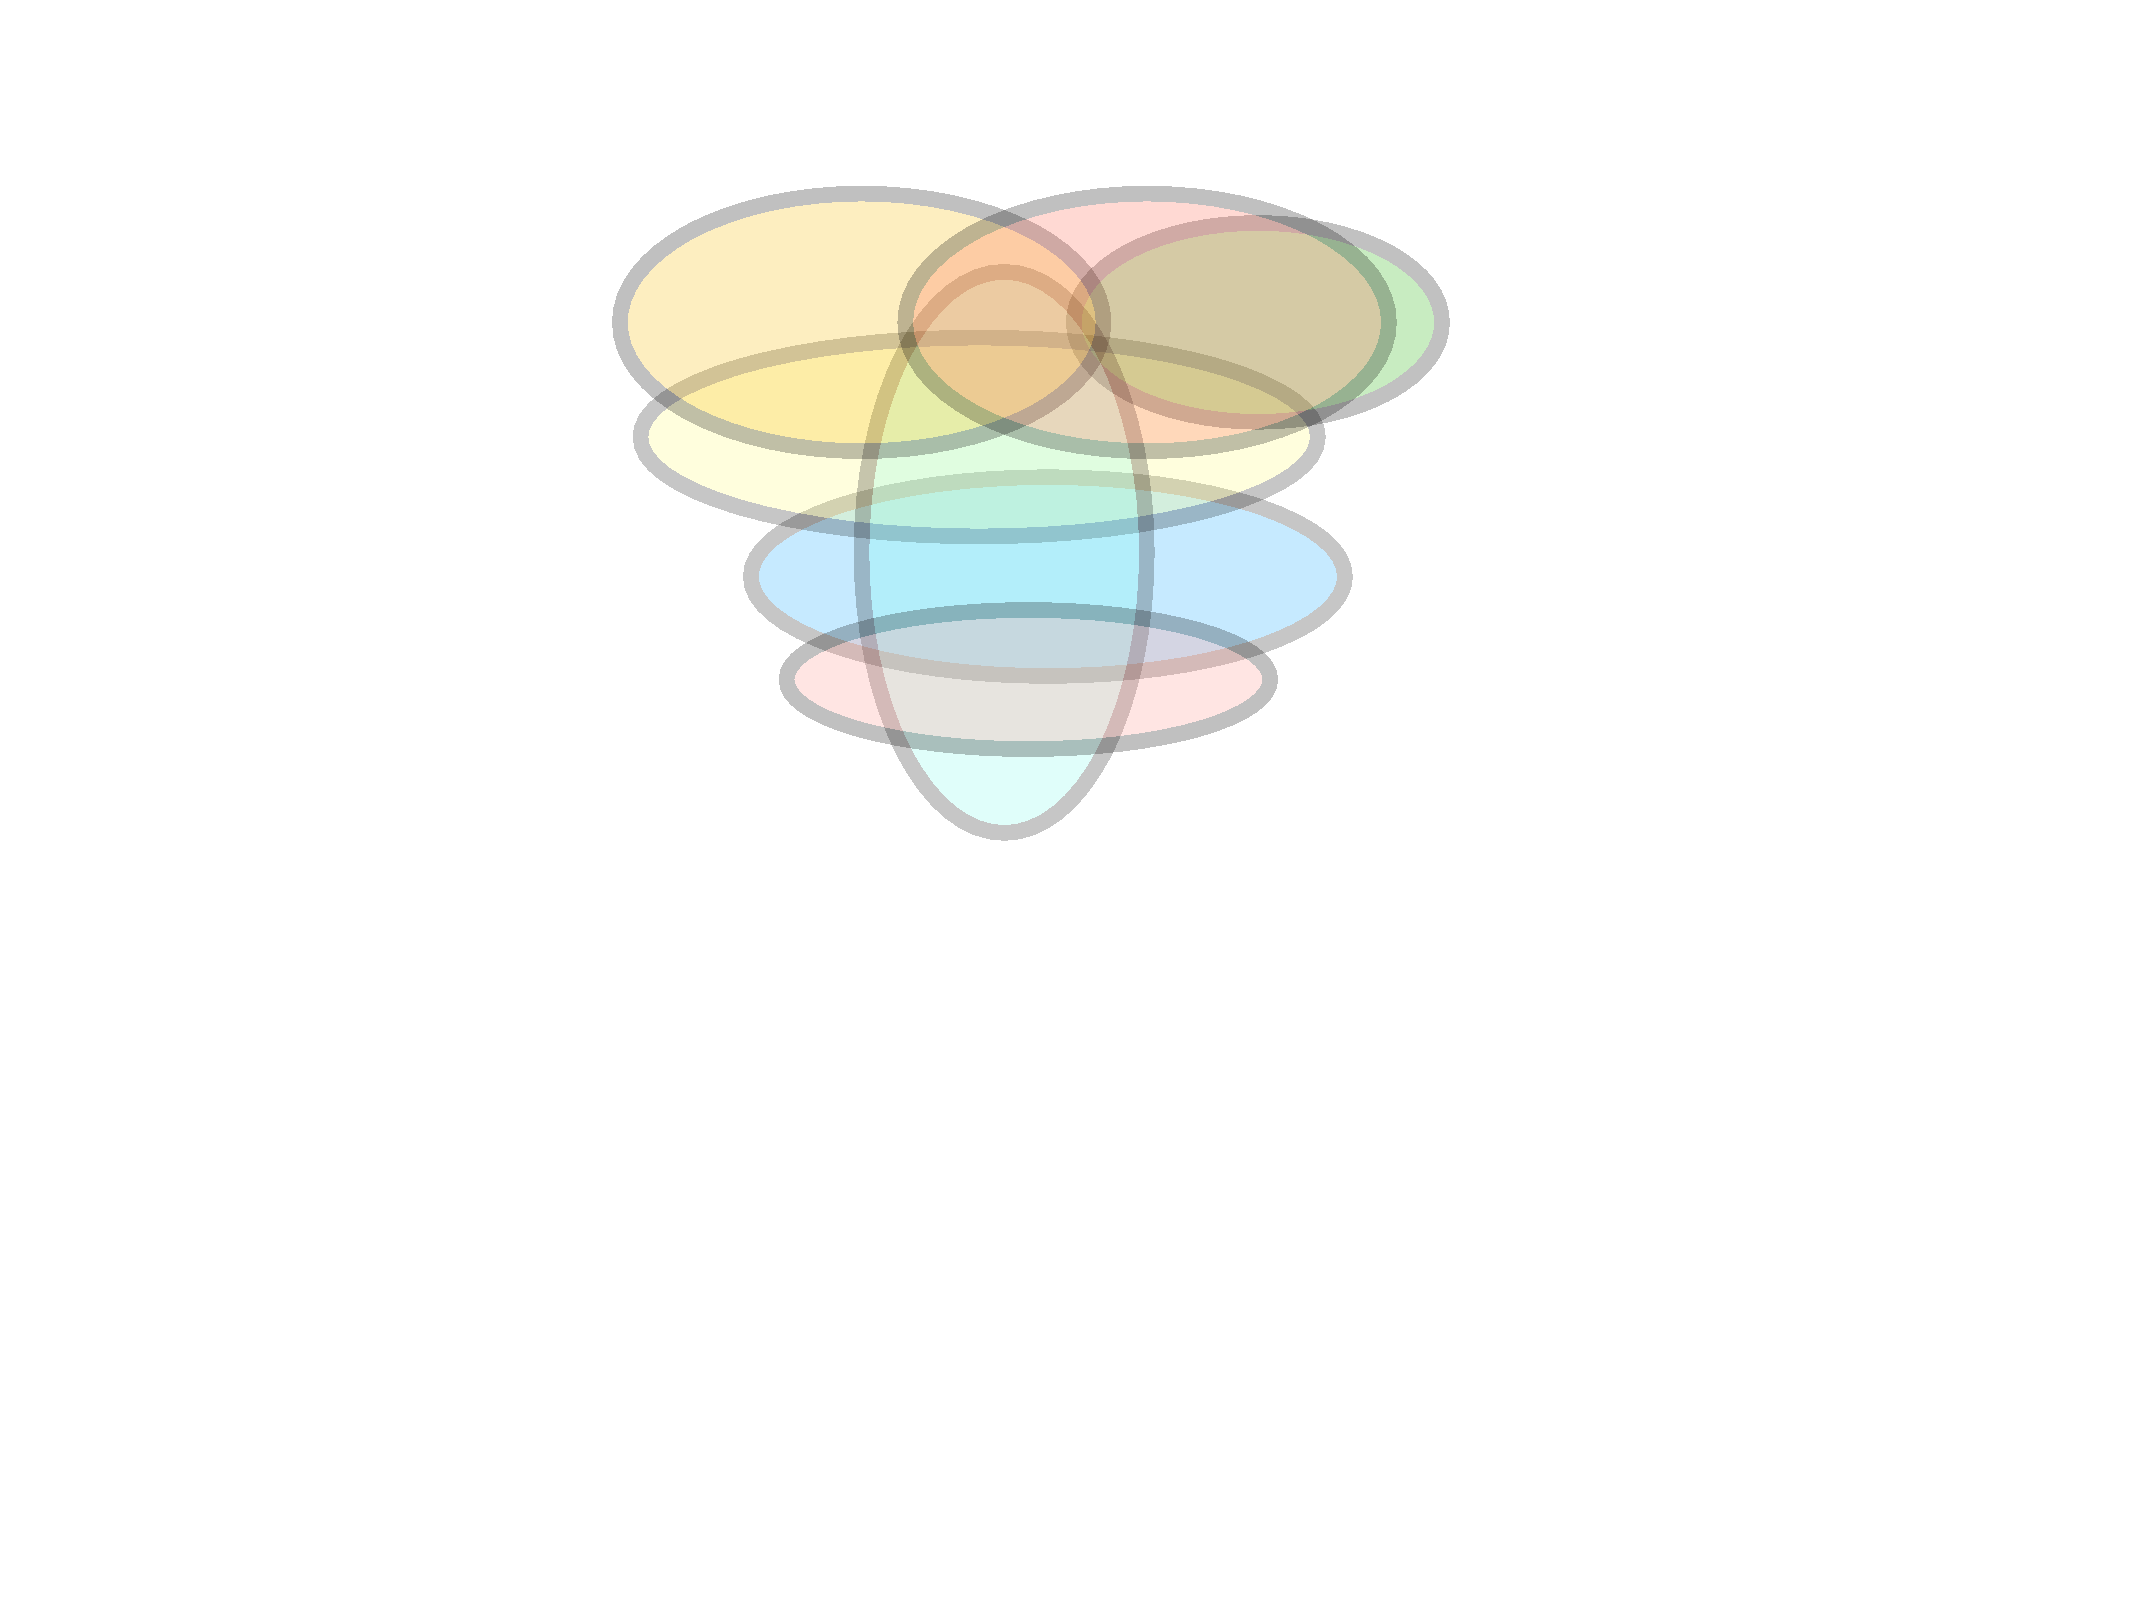
\includegraphics[width=\linewidth, trim=250  320 260 60,clip]{diagrams/Suff.pdf}
\end{minipage}
 & \ \ \ & 
\begin{minipage}{0.25\textwidth}
 
\includegraphics[width=\linewidth, trim=250  320 260 60,clip]{diagrams/Nec.pdf}
\end{minipage}
 & \ \ \ &
\begin{minipage}{0.25\textwidth}
 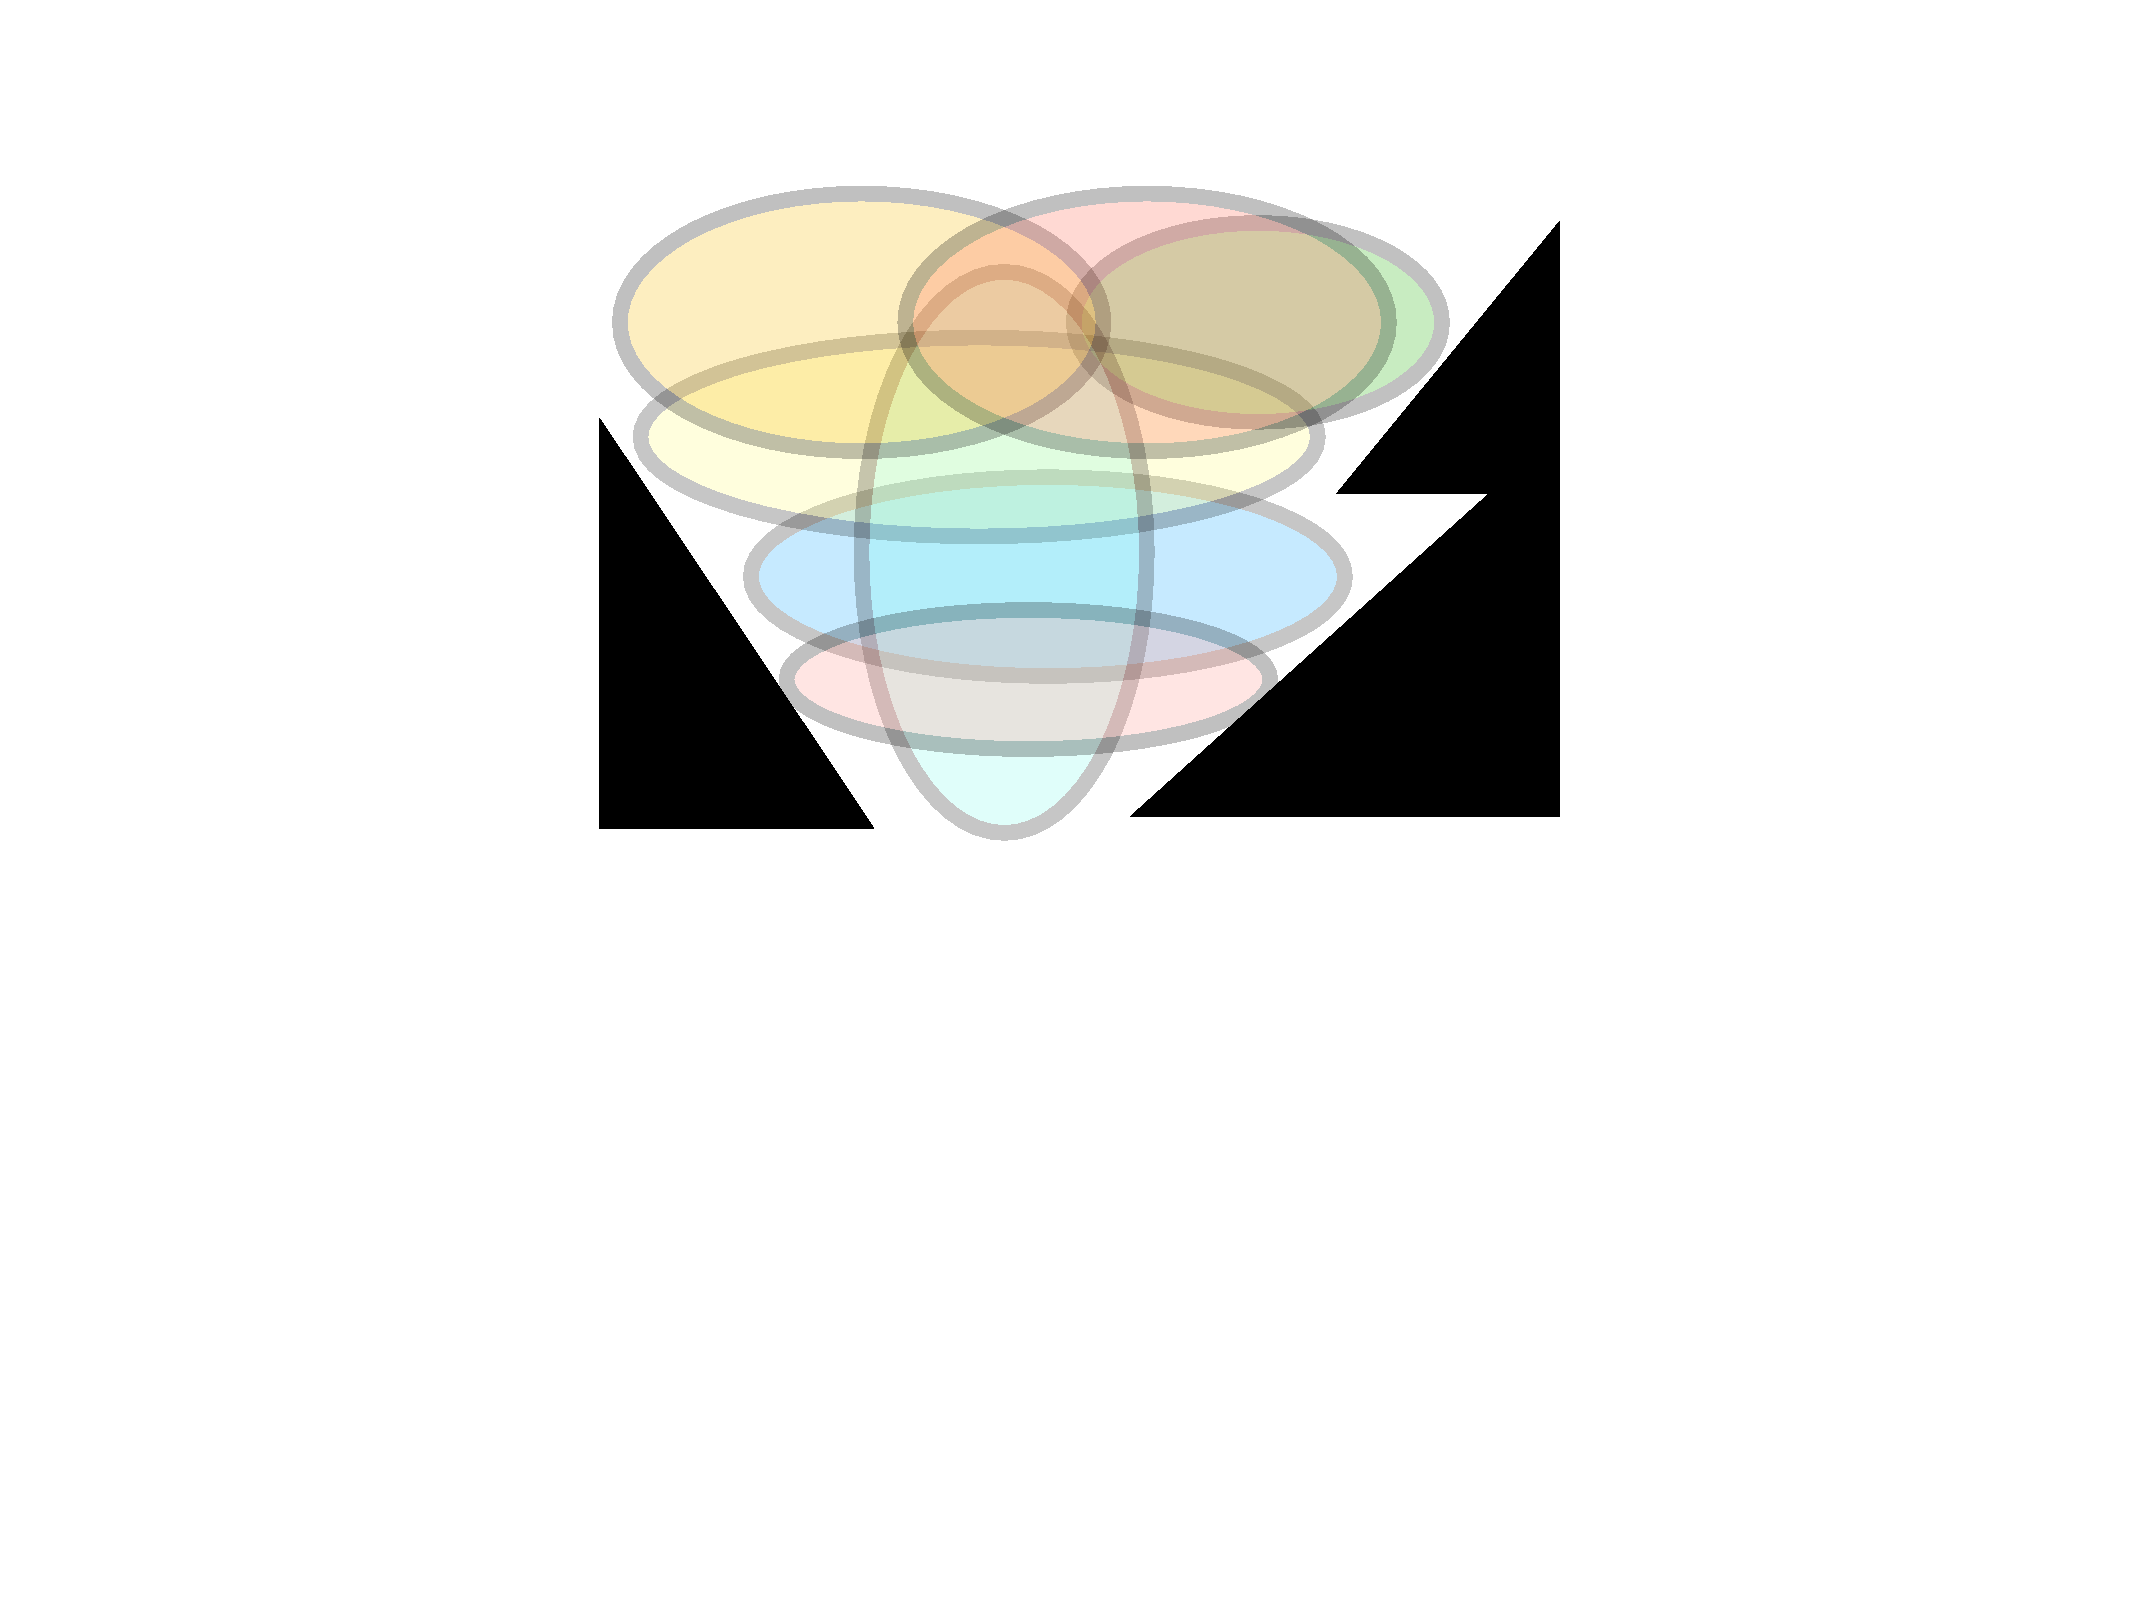
\includegraphics[width=\linewidth, trim=250  320 260 60,clip]{diagrams/NecAndSuff.pdf}
\end{minipage}
\\
sufficient  spec.& & necessary spec. & & holistic spec.
%\begin{minipage}{0.75\textwidth}
%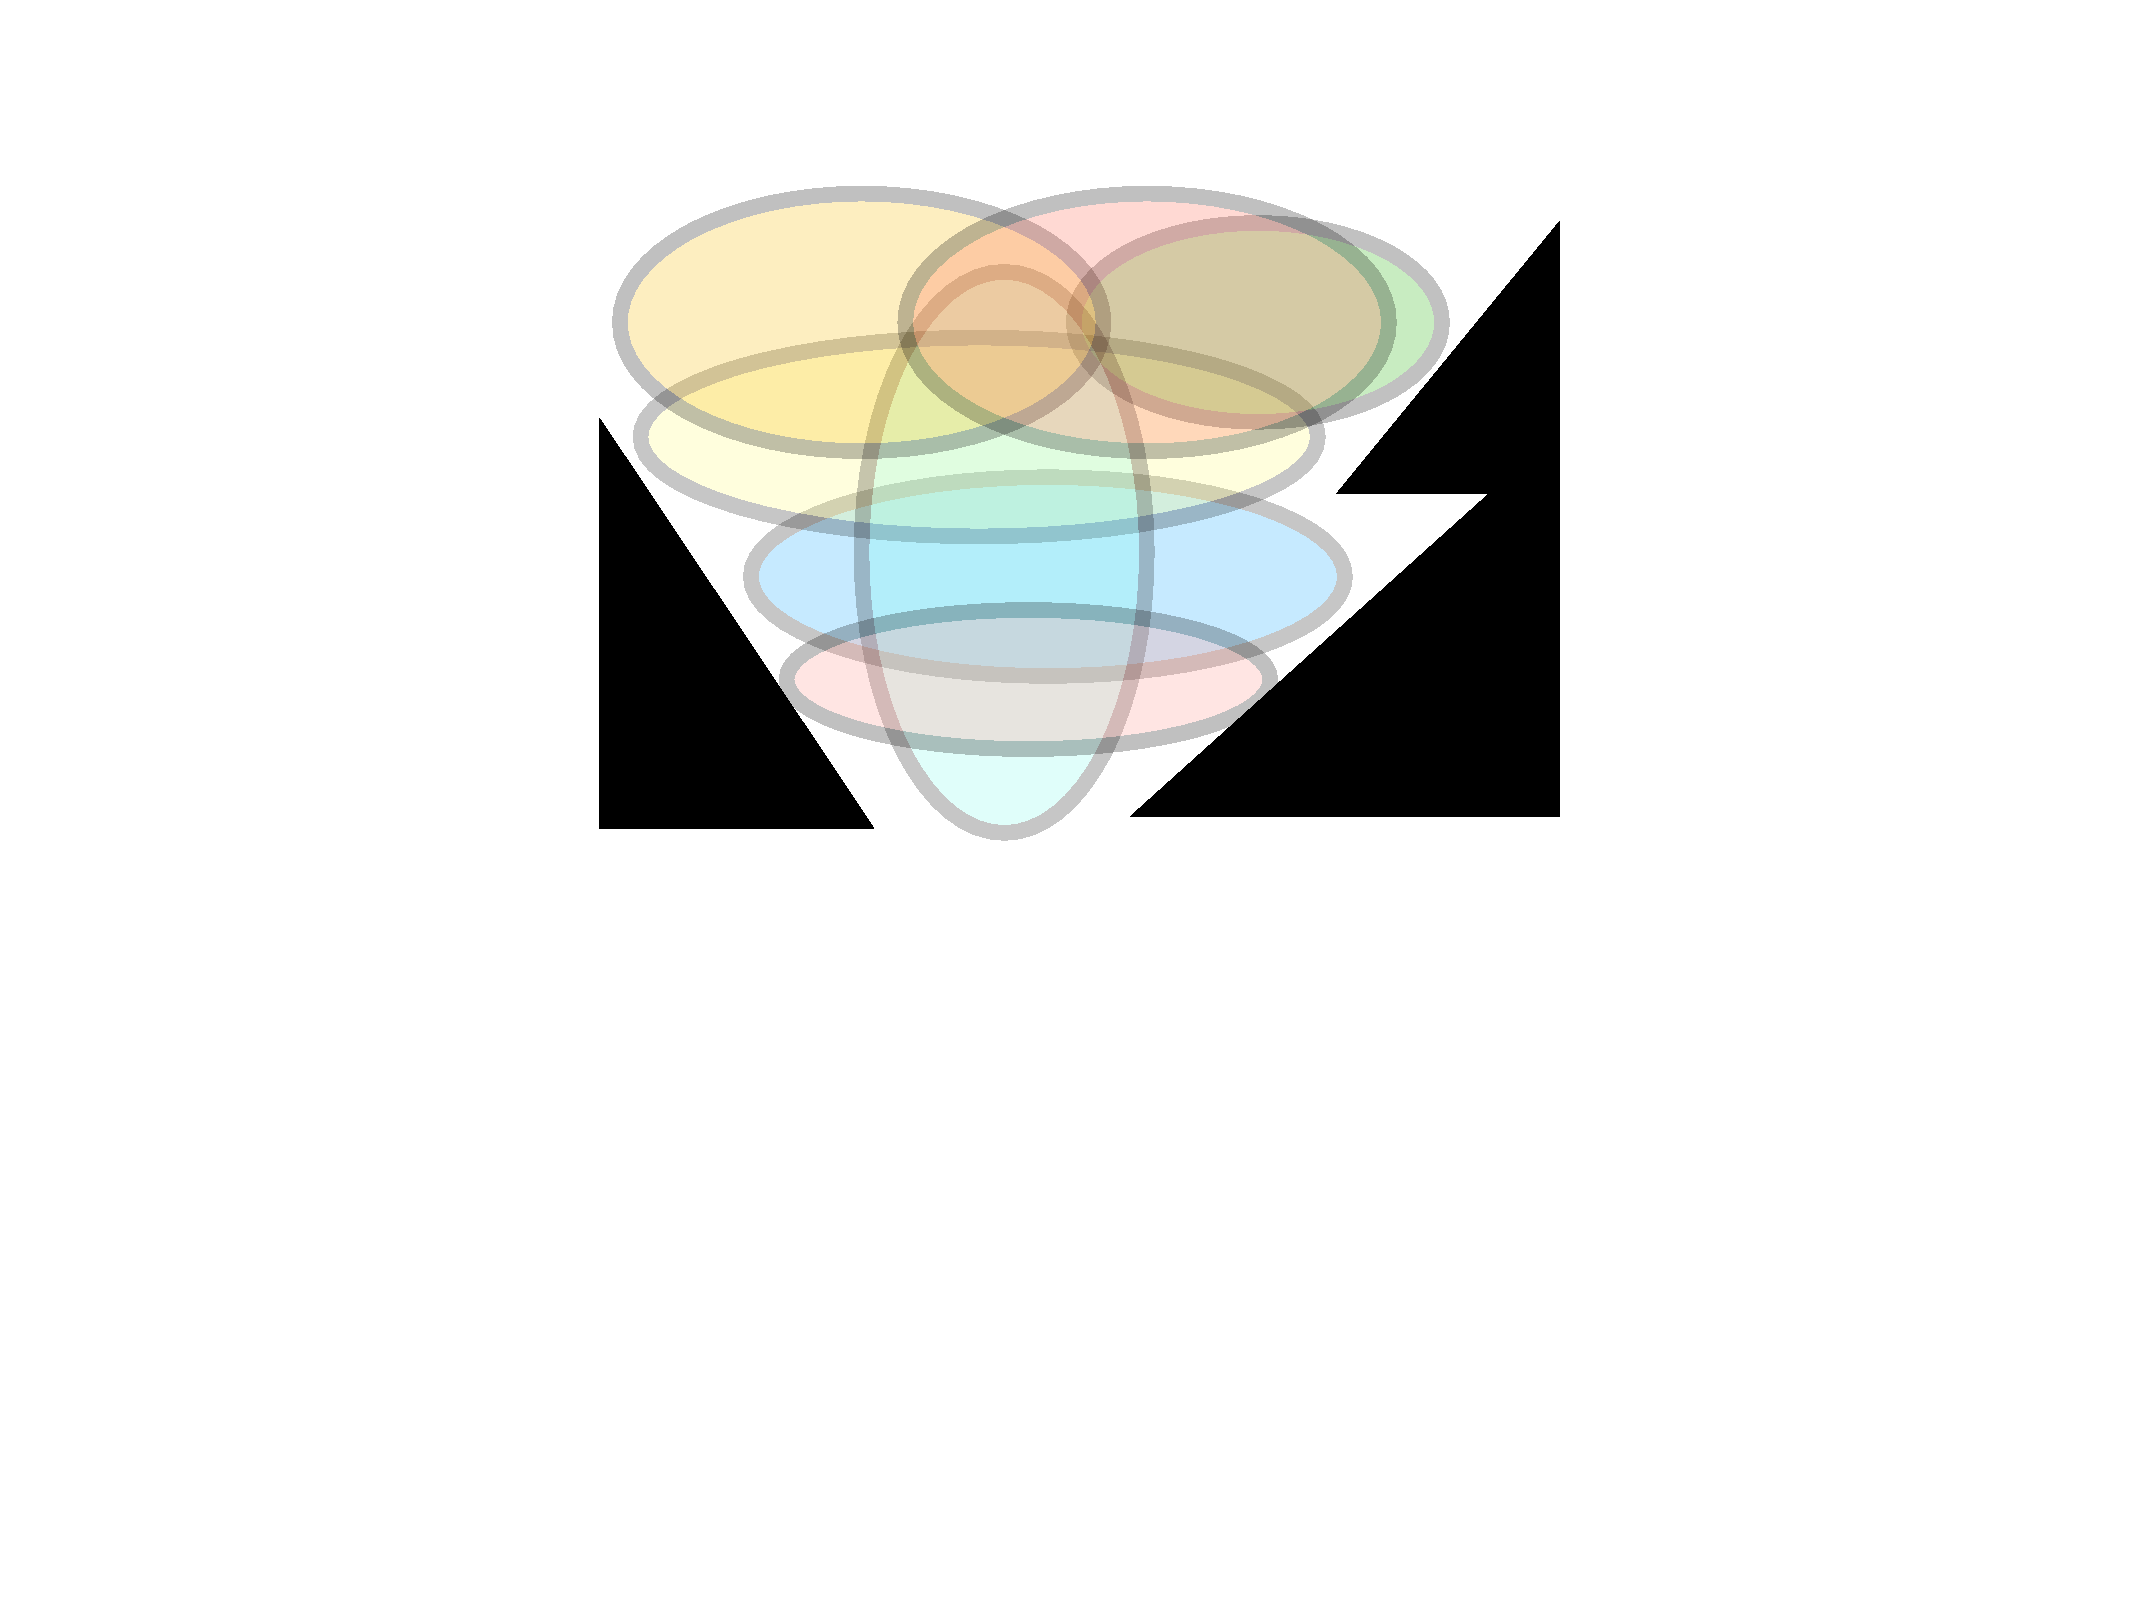
\includegraphics[width=\linewidth, trim=145  320 60 105,clip]{diagrams/NecAndSuff.pdf}
%\end{minipage}
%% y seems to eat up the bollom
%% x eats space from left, if you increase it the diagram decreases from left
%% w eats space from top, if you increase it the diagram decreases from top
%%\includegraphics[page=3, width=\linewidth, trim=150  270 40 150, clip]{diagrams/snmallocf.pdf}
%\sdcomment\sophia{I think we need to change the diagram so that it says small slab.}
%\end{minipage}
 \end{tabular}
  \vspace*{-2.5mm}
  \caption{Sufficient and Necessary Conditions, and Full Specifications}
 \label{fig:NecessaryAndSuff}
 \end{figure}
 
 We propose that  necessary conditions should be stated
 explicitly. Specifications should be \emph{holistic}, in the sense
 that they describe the  overall behaviour of a component: not only the
 behaviour of each individual functions, but also the 
 behaviour that emerges through combinations of functions.

Holistic specifications should therefore consist of   the sufficient as well as the necessary conditions, as  
depicted in right hand side  diagram in Fig. \ref{fig:NecessaryAndSuff}.
When a component has been specified holistically,  the behaviours
represented by the black triangles cannot occur, even when the
component interacts with other software of unknown provenance.
In Section \ref{sec:discussion} we argue why necessary conditions are more than the complement of
sufficient conditions.

Necessary conditions are guarantees upheld throughout program execution.
In this way, 
necessary conditions are closer to monitor or object
invariants \cite{Hoare74,Meyer97}. The difference between 
classical invariants and our holistic specifications is that classical invariants can only reflect  on
the current program state (\ie the contents of the
stack frame and the heap for an individual program component) while
holistic specifications reflect on all aspects of a program's
execution, potentially across all the components making up that program.


In this paper we propose \Chainmail, a specification language to
express holistic specifications.
%\james{has moved things around through here}
The design of \Chainmail was guided by the study of a sequence of
examples from the OCAP literature and the smart contracts world: the
membrane \cite{membranesJavascript}, the DOM \cite{dd,ddd}, the Mint/Purse \cite{MillerPhD}, the Escrow \cite{FTfJP14}, the DAO \cite{Dao,DaoBug} and
ERC20 \cite{ERC20}.  As we worked through the
examples, we found a small set of language constructs that let us
write holistic specifications across a range of different contexts.
%
 
While many individual features of \Chainmail can be found in other work, 
their power and novelty for specifying open systems lies in their careful combination.
In particular, \Chainmail extends 
traditional program specification languages\cite{Leavens-etal07,Meyer92} with features which talk about:
%
%\begin{description}
%\item[Permission] 
\ \ \textbullet \ \emph{Permission}, \ie which object may have access to which other objects; 
this is central since access to an object usually also grants access to the functions it provides.
%
\ \ \textbullet  \ \emph{Control}, \ie what  object called functions on other objects; this
 is useful in identifying the causes of certain effects - eg 
funds can only be reduced if the owner called a payment function.
%
%$\bullet$ \ \\emph{Authority}, \ie  which objects' state or properties may change; this is useful in describing effects, such as reduction of funds.
%
\ \ \textbullet \ \emph{Time}:\   \ie  what holds some time in  the past, the future, and what changes with time,
\ \ \textbullet \ \emph{Space}:\ \ie  which parts of the heap are considered when establishing some property, or when 
performing program execution; a concept
related to, but different from, memory footprints and separation logics,
\ \ \textbullet \ \sd{\emph{Viewpoints}:\ \ie  a distinction between the objects internal to our component, and those external to
it; a concept related to the open world setting.}
%\sophia{I do not know who wrote the comparison with foorprints, but it looks good to me.}
% end{description}

Holistic assertions often use several of these concepts. They often have the form of a guarantee
that if some property ever holds in the future, then some other property holds now, or that
certain effects can only caused by external objects with access to internal ones. \sophia{the first 4 sentences of this
para had been removed. But I modified them and like them. Waht do the others think?}
For example, if within a certain heap some change is possible in the future, then this particular heap contains 
at least one object which has access to a specific other, privileged object.
%\james{moved around --- not sure we need this para}
%\susan{I think we don't so there is a paragraph I have commented out.}
\forget{Ofte, holistic assertions typically have the form of a guarantee
that if some property ever holds in the future, then some other property holds now.
For example, if within a certain heap some change is possible in the future, then this particular heap contains 
at least one object which has access to a specific other, privileged object.}
A module\footnote{We use module and component in an analogous manner to class and object respectively.}
 satisfies a holistic assertion if, for all other modules,
  the assertion is satisfied  in all runtime configurations reachable through execution of the two modules combined.
  This reflects the open-world view.


\noindent The contributions of this paper are:\james{can we claim each of these?}\sophia{Yes to all, except for the last one --
not done yet. Do you think not?}
\begin{itemize}
\item the design of the holistic specification language \Chainmail,
\item the semantics of \Chainmail,
\item a validation of \Chainmail through its application to a sequence of examples,
\item a further validation of \Chainmail through informal proofs of adherence of code to some of these specifications.
\end{itemize}  
  
  
The rest of the paper is organized as follows: Section~\ref{sect:motivate:Bank} 
motivates our work in terms of an example. Sections~\ref{sect:LangOO} contain a formal definition of \LangOO, and Section~\ref{sect:assertions} the semantics of assertions. Section ... related work .... Section xxxx concludes.
\kjx{TODO AT THE END}



\section{Motivating Example: The Bank}
\label{sect:motivate:Bank}
%\kjx{removed para that mostly duplicated intro}  
%% Traditional functional specifications describe what objects are
%% guaranteed to do. 
%% So long as a method is called in a state satisfying
%% its preconditions, the method will complete its work and establish a
%% state satisfying its postconditions.  
%% Thus, the precondition and the method call together form a \emph{sufficient}
%% condition for the method's effect.
% SD The below is wrong:
% Method specifications thus
% define the \textit{sufficient} conditions for their methods' behaviour
% to be invoked.

As a motivating example, we consider a simplified banking application,
with objects representing \prg{Account}s or \prg{Bank}s. 
As in \cite{ELang},   \prg{Account}s belong to \prg{Bank}s and hold money (here \prg{balance}s);  
with access  to two \prg{Account}s of the same  \prg{Bank} one can  transfer any amount of money from
 one to the other.  We give a traditional specification in Figure \ref{fig:BankSpec}.

%SD changed function to method, to fir what comes later.
\begin{figure}[htbp] 
\begin{lstlisting}
   method deposit(src, amt)
   PRE:  this,src:Account $\wedge$  this$\neq$src $\wedge$ this.myBank=src.myBank $\wedge$ 
         amt:$\mathbb{N}$  $\wedge$   src.balance$\geq$amt
   POST: src.balance=src.balance$\pre$-amt $\wedge$ this.balance=this.balance$\pre$+amt

   method makeNewAccount(amt)
   PRE: this:Account $\wedge$  amt:$\mathbb{N}$ $\wedge$  this.balance$\geq$amt
   POST: this.balance=this.balance$\pre$-amt $\wedge$ fresh result $\wedge$ 
         result: Account $\wedge$ this.myBank=result.myBank $\wedge$ result.balance=amt

   method newAccount(amt)
   PRE:  this:Bank  
   POST:  result: Account $\wedge$  result.myBank=this $\wedge$ result.balance=amt
 \end{lstlisting}
 \vspace{-.8cm}
\caption{Functional specification of \prg{Bank} and \prg{Account}
%
}
\label{fig:functionalSpecBankAccount}
\label{fig:BankSpec}
\end{figure} 

The PRE-condition of \prg{deposit} requires that  the receiver and the
first argument  (\prg{this} and \prg{scr}) are \prg{Account}s
and belong to the same bank,
that the second argument \prg{amt} is a number, and that \prg{src}'s
balance is least \prg{amt}.
The POST-condition mandates that \prg{amt} has been transferred from \prg{src} to the receiver.
 The function \prg{makeNewAccount}  returns a fresh \prg{Account} with the same bank, and transfers \prg{amt}
 from the receiver \prg{Account} to the new \prg{Account}.
 Finally, the function \prg{newAccount} when run by a \prg{Bank} creates a new \prg{Account} with corresponding 
 amount of money in it. \footnote{ \se{Note that our very simple bank doesn't even have a concept of owner of an account.}}
% \se{As specified in our \prg{BankSpec} the only way to put money into the \prg{Bank} is with a call to \prg{newAccount} and there is no way to remove money from the \prg{Bank}.}\sophia{We can say that, but is it important? We do not even use "newAccount" anywhere}

\forget{
\emph{Aside} Notice that the specification means that access to an \prg{Account} allows anyone to withdraw all the money it holds
-- the concept of account owner who has exclusive right of withdrawal is not supported.
This simplified view allows  us to keep the example short, but compare with appendix \sophia{TO ADD}
for a specification which supports owners. \emph{end aside}\sophia{which is the best place to say that?}
}

With such a specification %it is enough%to let us
%calculate the result of operations on the accounts ---
%for example % it is straightforward to determine that 
the code below  satisfies its assertion: assuming that 
\prg{acm\_acc} and \prg{auth\_acc} are \prg{Account}s for the ACM and
for a conference paper author respectively. The ACM's \prg{acm\_acc}
has a balance of 10,000 before an author is 
registered. but afterwards it has a balance of 11,000. Meanwhile the
\prg{auth\_acc}'s balance  will be 500 from a starting balance of 1,500
(barely enough to buy a round of drinks at the conference hotel bar).

\begin{lstlisting}
  assume acm_acc,auth_acc: Account $\wedge$ acm_acc.balance=10000 $\wedge$  auth_acc.balance=1500
  acm_acc.deposit(auth_acc,1000)
  assert acm_acc.balance=11000  $\wedge$ auth_acc.balance=500
\end{lstlisting}

\vspace{-.2in}

This reasoning is fine in a closed world, where we only have to
consider complete programs, where all the code in our programs (or any
other systems with which they interact) is under our control.   
In an
open world, however, things are more complex: our systems will be made
up of a range of 
%modules, 
components, many of which we do not control; and
furthermore will have to interact with external systems which we
certainly do not control.  Returning to our author, say some time
after registering by executing the \prg{deposit} code above, they
attempt to pay for a round at the bar.  Under what circumstances can
they be sure they have enough funds in their account?

To see the problem, what if the bank provided a \prg{steal} method that 
 emptied out every account in the bank into a thief's account.
 %\se{(also in the \prg{Bank})}?\sophia{yes, also in the bank, but does ti matter? I want to avoud having too many facets in the story.}
%all their funds into the thief's account.
%consider the additional function specified below.
% The bank additionally provides a
%\prg{steal} method that empties out every account in the bank and puts
%all their funds into the thief's account. 
If this method existed and
if it were somehow called between registering at the conference and
going to the bar, then the author 
%(actually everyone using the same bank)
%would find an empty account (as would every other account holder other than the thief, of course).
would find an empty account.
\susan{I have removed the statements that implied people had accounts because we don't have that in the spec}
%

%\vspace{-2in}
%\begin{lstlisting}
%   function steal(thief)
%   PRE:  this:Bank $\wedge$  thief.myBank=this 
%   POST: $\forall$a:Account.[a.myBank=this $\rightarrow$ a.balance=0 ] $\wedge$ 
%         thief.balance=thief.balance$\pre$+$\sum_{\prg{a}:\prg{Account} \wedge \prg{a.myBank}=\prg{this}}$ a.balance$\pre$
% \end{lstlisting}
%\vspace{-2in}
 
The critical problem is that a bank implementation including a \prg{steal}
method would meet the functional specification of the bank from
fig.~\ref{fig:functionalSpecBankAccount}, so long as the methods \prg{deposit},
\prg{makeNewAccount}, and \prg{newAccount}    meet
their specification.

One obvious solution would be to return to a closed-world
interpretation of specifications: we interpret specifications such as
fig.~\ref{fig:BankSpec} as \emph{exact} in the sense that only
implementations that meet the functional specification exactly,
\emph{with no extra methods or behaviour}, are considered as suitable
implementations of the functional specification. The problem is that
this solution is far too strong: it would for example rule out a bank
that  during software maintenance was given a new method \prg{count}
that simply counted the number of deposits that had taken place, or a method \prg{notify}
to enable the bank to occasionally send notifications  to its customers.
% occasionally paid interest to its clients.
%i.e. met fig.~\ref{fig:extras} as well as fig.~\ref{fig:BankSpec}.
%
%\begin{figure}[tbp]
%\begin{lstlisting}
%   function deposit(src, amt)
%   PRE:  $\mbox{ ... as before ...}$  
%   POST:  $\mbox{ ... as before ...}$  this.myBank.count=this.myBank.count$\pre$+1
% \end{lstlisting}
%\vspace{-.8cm}
%\caption{Counting deposits} %and paying interest}
%\label{fig:extras}
%\end{figure} 
% removed as payInterest affects the balance
%
%   function payInterest()
%   PRE: this:Bank  
%   POST: $\forall$a:Account.[a.myBank=this $\rightarrow$ a.balance=a.balance$\pre$+a.balance$\pre$/1000]


What we need is some way to permit bank implementations that 
%meet fig.~\ref{fig:extral} 
send notifications to customers but to forbid implementations of \prg{steal}. % that meet fig.~\ref{fig:steal}.  
The key here is to capture the (implicit)
assumptions underlying fig.~\ref{fig:BankSpec}, and to provide
additional specifications that capture those assumptions.  The following
 three informal requirements   prevent methods like \prg{steal}:

\begin{enumerate}
\item % After creation,
% it said
%  the \emph{only} way and account -- SD chnaged as I thibk ti has slifghtly wrong meaning 
An account's
  balance can be changed only  if a client   calls the \prg{deposit} method  with the
  account as the receiver or as an argument. 
 % \sophia{I changed the wording as I want to show "change -> call to deposit"}
%  \susan{point out that this is not sufficient to stop steal because it could be rewritten to use deposit.}
%  \sophia{I think that is what we say below}
\item An account's balance can be changed  only  if a client has
  access to that  particular account. % object.
  % I want the structure of (1) and (2) to be similar.
\item The \prg{Bank}/\prg{Account} component cannot leak access to existing accounts or banks. 
%SD I chnaged the belwo
%Neither accounts nor banks can leak money.   \susan{ I changed what you had in point 3 because it didn't make sense in context. I don't think what I put is what you were saying is it? Did you want to say something like 'There is no way that references to either accounts or banks can be passed to third parties?}
\end{enumerate}

Compared with the functional specification we have seen so far, these
requirements %assumptions 
capture \emph{necessary} %conditions 
rather than
\emph{sufficient} conditions:  Calling the \prg{deposit}
method to gain access to an account %is called to change an account's balance, and it is necessary
is necessary for any change to that account taking place.
%that the particular account object can be passed as a parameter to
%that method. 
The  function 
\prg{steal} is inconsistent with requirement  (1), as it reduces the balance of an \prg{Account} without calling the
function \prg{deposit}. 
However, requirement  (1) is not enough to protect our money. We need to (2) to avoid an \prg{Account}'s balance getting
modified without access to the particular \prg{Account}, and (3) to ensure that such accesses are not leaked. 

%\james{NEED TO DECIDE ON CONTRIBUTIONS.
%The contribution of this paper is a specification langauge and
%semantics that can be used to specify necessary specifications, and a
%semantics for those specifications that can determine whether some
%functional (sufficient) specifications are consistent (or not) with
%the necessary specifications. Also think that we do not do
%"can determine whether some
%functional (sufficient) specifications are consistent (or not) with
%the necessary specifications."}

 
We can  express these  requirements  %assumptions using 
through \Chainmail assertions.  Rather than %specifying \prg{functions} to  describe
specifying the behaviour of particular methods when they are called, we
write  invariants   that range across the entire behaviour of the
\prg{Bank}/\prg{Account}  module:
\vspace{.2cm}

%\begin{figure}[htbp]
%%\begin{definition}
%\label{def:pol2}

(1)\ \  $\triangleq$\ \ $\forall \prg{a}.[\ \ \prg{a}:\prg{Account} \wedge \Changes{\prg{a.balance}}  \ \    
    \longrightarrow \ \    \hfill$ \\
  $\strut \hspace{2.3cm} 
% TODO explain:
% we no longer need Past here, as we are ion visible states 
  \exists \prg{o}. [\    \Calls{\prg{o}}{\prg{deposit}}{\prg{a}}{\_} \vee\  \Calls{\prg{o}}{\prg{deposit}}{\_}{\prg{a}}\  \ ] \ \ \ \ ] \hfill $

\vspace{.4cm}

    (2)\ \  $\triangleq$\ \ $\forall \prg{a}.\forall \prg{S}:\prg{Set}.\ [  \ \  \prg{a}:\prg{Account}\ \wedge \  \Using{ \Future{\,\Changes{\prg{a.balance}}} \,}{\prg{S}\,}\ \ \   \
    \longrightarrow$ \\
 $\strut \hspace{3.9cm} \hfill \exists \prg{o}.\ [\, \prg{o}\in \prg{S}\ \wedge\  \External{\prg{o}}  \ \wedge \ \CanAccess{\prg{o}}{\prg{a}} \, ] \ \ \ \ ]$
\vspace{.4cm} 
 
     (3)\ \  $\triangleq$\ \ $\forall \prg{a}.\forall \prg{S}:\prg{Set}.\ [ \ \  \prg{a}:\prg{Account}\ \wedge \ \ {\Using{\Future{\ \exists \prg{o}.[\ \External{\prg{o}} \ \wedge\ \CanAccess{\prg{o}}{\prg{a}}]}}{\SF}}$ \\  
 $\strut \hspace{3.9cm} \hfill   \longrightarrow \ \ \ \exists \prg{o}'.\ [\, \prg{o}'\in \prg{S}\  \wedge  \ \External{\prg{o}'}  \ \wedge \ \CanAccess{\prg{o}'}{\prg{a}}   \ ] \ \ \ \ ]$

%\end{definition}
%\vspace{-.2cm}
%\caption{Necessary specifications for \prg{deposit}}
%%\label{fig:nec}
% \end{figure}
\vspace{.2cm}

%% We will discuss the meaning of  \Chainmail assertions in more detail in the next sections, but 
%% give here a first impression, and discuss (1)-(3):
 
Assertion (1) %in fig.~\ref{fig:nec} says 
says that if   an account's balance changes
($\Changes{\prg{a.balance}}$),
then there must be some client object \prg{o}
that % in the past (${\Past{...}}$) 
called the \prg{deposit} method with \prg{a} as a receiver or as an argument 
($\Calls{\prg{o}} {\prg{deposit}} {\_} {\_}$).
\sophia{ explain in some later section on that  this assertion
implicilty gives   that \prg{o} is external \kjx{why: it explicitly says
``external(o)''}}
%bank and its associated accounts ($\prg{o} \notin\prg{Internal}(\prg{a})$)" -- and I have chopped it from
%the spec. This is because of the visible states :-)}
 
Assertion (2) similarly constrains any possible change to an 
account's balance: 
If at some future point the balance changes  (${\Future{\,\Changes{...}}}$),  % (${\Future{...}}$) %
and if this future change is observed with the state restricted to the objects from \SF~ (\ie $\Using{...}{\prg{S}}$), then 
at least one of these objects ($\prg{o}\in\SF$) is external to the \prg{Bank}/\prg{Account} system ($\External{\prg{o}}$) and 
has (direct) access to that account object
($\CanAccess{\prg{o}}{\prg{a}}$).
Notice that while the change in the \prg{balance} happens some time in the future,
the external object \prg{o} has access to \prg{a} in the \emph{current} state.
Notice also, that the object which makes the call to \prg{deposit} described in (1), and the object which 
has access to \prg{a} in the current state described in (2) need not be the same: It may well be that the
latter passes (indirectly) a reference to \prg{a} to the former, which then   makes the call
to \prg{deposit}.

It remains to think about how access to a \prg{Account} may be obtained. This is the remit of assertion (3): 
\sd{It} says that if at \sd{some time} in the future of the state restricted to \SF, 
some object \prg{o} which is external has access to some account \prg{a}, and if \prg{a} exists in the 
current state, then in the current state some object 
from \SF~has access to \prg{a}. Note that \prg{o} and $\prg{o}'$ may but need not be the same object. Note also
that $\prg{o}'$ has to exist and have access to \prg{a} in the current state, but 
\prg{o} need not exist in the current state -- it may be allocated later.

\vspace{.1cm}

A  holistic  specification for the bank account, then,
would be our original sufficient functional specification from
fig.~\ref{fig:BankSpec} plus the necessary
%security policy
specifications (1)-(3) from above. %in fig.~\ref{fig:necBank}.   
This holistic specification
permits an implementation of the bank that also provides  \prg{count}
and \prg{notify} methods: the specification does not mention either method.
Critically, though, the \Chainmail specification
does not permit an
%specification from fig.~\ref{fig:count},
implementation that includes a \prg{steal} method.
\sophia{We said this earlier, do we repeat? \kjx{no, cos this time we're
saying it in chainmail..?}} 
First, the \prg{steal} method clearly changes the balance of
every account in the bank, but policy (1) requires that any method
that changes the balance of any account must be called \prg{deposit}.
Second, the \prg{steal} method changes the balance of every account in
the system, and will do so without the caller having a reference to
most of those accounts, thus breaching policy (2).   
% SD chopped. unnecessary
%Note that \prg{steal} putting all the funds into the thief's account
%does not breach policy (2) with respect to the thief's own account,
%because that account is passed in as a parameter to the \prg{steal}
%method, and so the called of the \prg{steal} must have access to that
%account.
 
Assertion (3) gives essential protection when dealing with foreign, untrusted code.
% \sophia{I like the story of this paragraph. Please make more eloquent.}
\sophia{Assertion (3) is a corollary of (2), and thus actually superfluous -- do we say that?
Do we say the story just using (2)?}
\susan{I think having 1 and 2 would make it more complicated. You could have a footnote though that says actually you don't even need 3 as it is a corollary of 2}
When an \prg{Account} is given out to untrusted third parties, assertion (3) guarantees that
this \prg{Account} cannot be used to obtain access to further  \prg{Account}s. 
The \prg{ACM} does not trust its authors, and certainly does not want
to give them access to \prg{acm\_acc}, which contains all of
the \prg{ACM}'s money. Instead, in order to receive money, it will
pass a secondary account used for incoming funds, \prg{acm\_incoming},
into which an \prg{author}  will pay the fee, and from which the \prg{ACM} will transfer the money
back into the main \prg{acm\_acc}. Assertion (3) is crucial, because it guarantees that even 
malicious authors  could not use knowledge of  \prg{acm\_incoming} to obtain access to
the main \prg{acm\_acc} or any other account. %, to which she did not have access.

\forget{
\sd{Thus, we need to be able to argue, that  passing the \prg{acm\_incoming to some unknown object \prg{u},
with an unknown function \prg{mystery}, is guaranteed not to affect \prg{acm\_acc} , unless \prg{u} already has
access to \prg{acm\_acc} before the call. With holistic assertions we can make this argument formally, while
with traditional specifications we cannot.}}
}
 
\vspace{.1cm} 

In summary, our  necessary specifications are invariants that describe the
behaviour of a module as observed by its clients. 
\forget{in fact, in section XXX\sophia{TO ADD} we show two very different implementations
of the \prg{Bank}/\prg{Account} specification which also satisfy (1)-(3).}
Our invariants 
 can talk about space, time and control, and thus go beyond
%can be defined and interpreted independently of any particular
%implementation of a specification --- rather our policies constrain
%implementations, in just the same way as traditional functional
%specifications. 
 %This is in contrast to e.g.\ 
 class invariants, which can only
talk   about relations between the  values of the fields of the objects.
%\sophia{This is james' original point, made a bit more concrete. Please check whether it makes sense.}
% of a module.
% invariants across the implementation of an abstract, or
% abstraction functions, which link an abstract model to a concrete
% implementation of that model. 
As our invariants are (usually) independent of a concrete implementation details they do not constrain the code to a specific implementation.


\section{\Chainmail\ Overview}
\label{sect:chainmail}
%
% SD removed as we said it earlier already
%%%(\eg  \prg{a1}.\prg{myBank} = \prg{a2}.\prg{myBank}),   %kjx elided
%%
%%
%\Chainmail\ incorporates assertions   about
%%\susan{the intro mentions viewpoint as well - the two should be consistent}
%%
%\textit{permission},
%% --- objects being accessible from other objects (\eg
%% $\CanAccess{\x}{\y}$);
%%
%\textit{control},
%% --- the next method to be invoked ($\Calls {\x} {\y} {\m} {\z}$);
%%
%%\textit{authority},
%%  --- about the change of some property (\eg $\Changes{\x.\f}$);
%%
%\textit{space}, %--- some property being observable within a subset of
%%the current state ( $\Using{\A}{S}$);
%%
%\textit{time},
%%
%and \textit{viewpoint},
%% --- about some property holding in the future or in the past (\eg $\Future \A$ or $\Past \A$).
%%
%as well as   ``classical'' assertions \sophia{would be nice iof we had a better name}
%about  variables and the heap.
%%
In this section we give a brief and informal  overview of some of the most salient features of  
\Chainmail -- a full exposition appears in Section \ref{sect:assertions}.



\sdparagraph{Example Configurations} We  will illustrate these features using the  \prg{Bank}/\prg{Account} example from the previous section.
We   use the runtime configurations $\sigma_1$ and $\sigma_2$ 
shown in the left and right diagrams in Figure \ref{fig:BankAccountDiagrams}. 
%These configurations could arise from the execution of different implementation of the \prg{Bank}/\prg{Account}
% module.
In both diagrams the rounded boxes depict objects:  green for those from the 
\prg{Bank}/\prg{Account} component, and grey for the ``external'',  ``client'' objects.
The light green area shows which objects are contained by the \prg{Bank}/\prg{Account} component.
The object at \prg{1} is a \prg{Bank}, those at \prg{2}, \prg{3} and \prg{4} are 
\prg{Account}s, and those at \prg{91}, \prg{92}, \prg{93} and \prg{94} are 
``client'' objects which belong to classes not from the \prg{Bank}/\prg{Account}  module.

Each configuration represents one alternative implementation of the Bank object.
Configuration  $\sigma_1$ may arise from execution using a module $M_{BA1}$, where  \prg{Account} objects
  have a field \prg{myBank} pointing to their \prg{Bank}, and an integer field  \prg{balance}
-- the code can be found in appendix~\ref{Bank:appendix} Fig.~\ref{fig:BanAccImplV1}.
Configuration  $\sigma_2$ may arise from execution using a module $M_{BA2}$,  where \prg{Account}s have a \prg{myBank}
field,  \prg{Bank} objects  have a \prg{ledger} implemented though a sequence of \prg{Node}s, each of which has a
 field pointing to an \prg{Account}, a field \prg{balance}, and a
 field \prg{next} -- the code can be found in appendix~\ref{Bank:appendix}
Figs.~\ref{fig:BanAccImplV2a} and~\ref{fig:BanAccImplV2b}.

 
 
\begin{figure}[htbp]
\begin{center}
\begin{tabular}{cc}
 \begin{minipage}{0.45\textwidth}
$\sigma_1$\\
 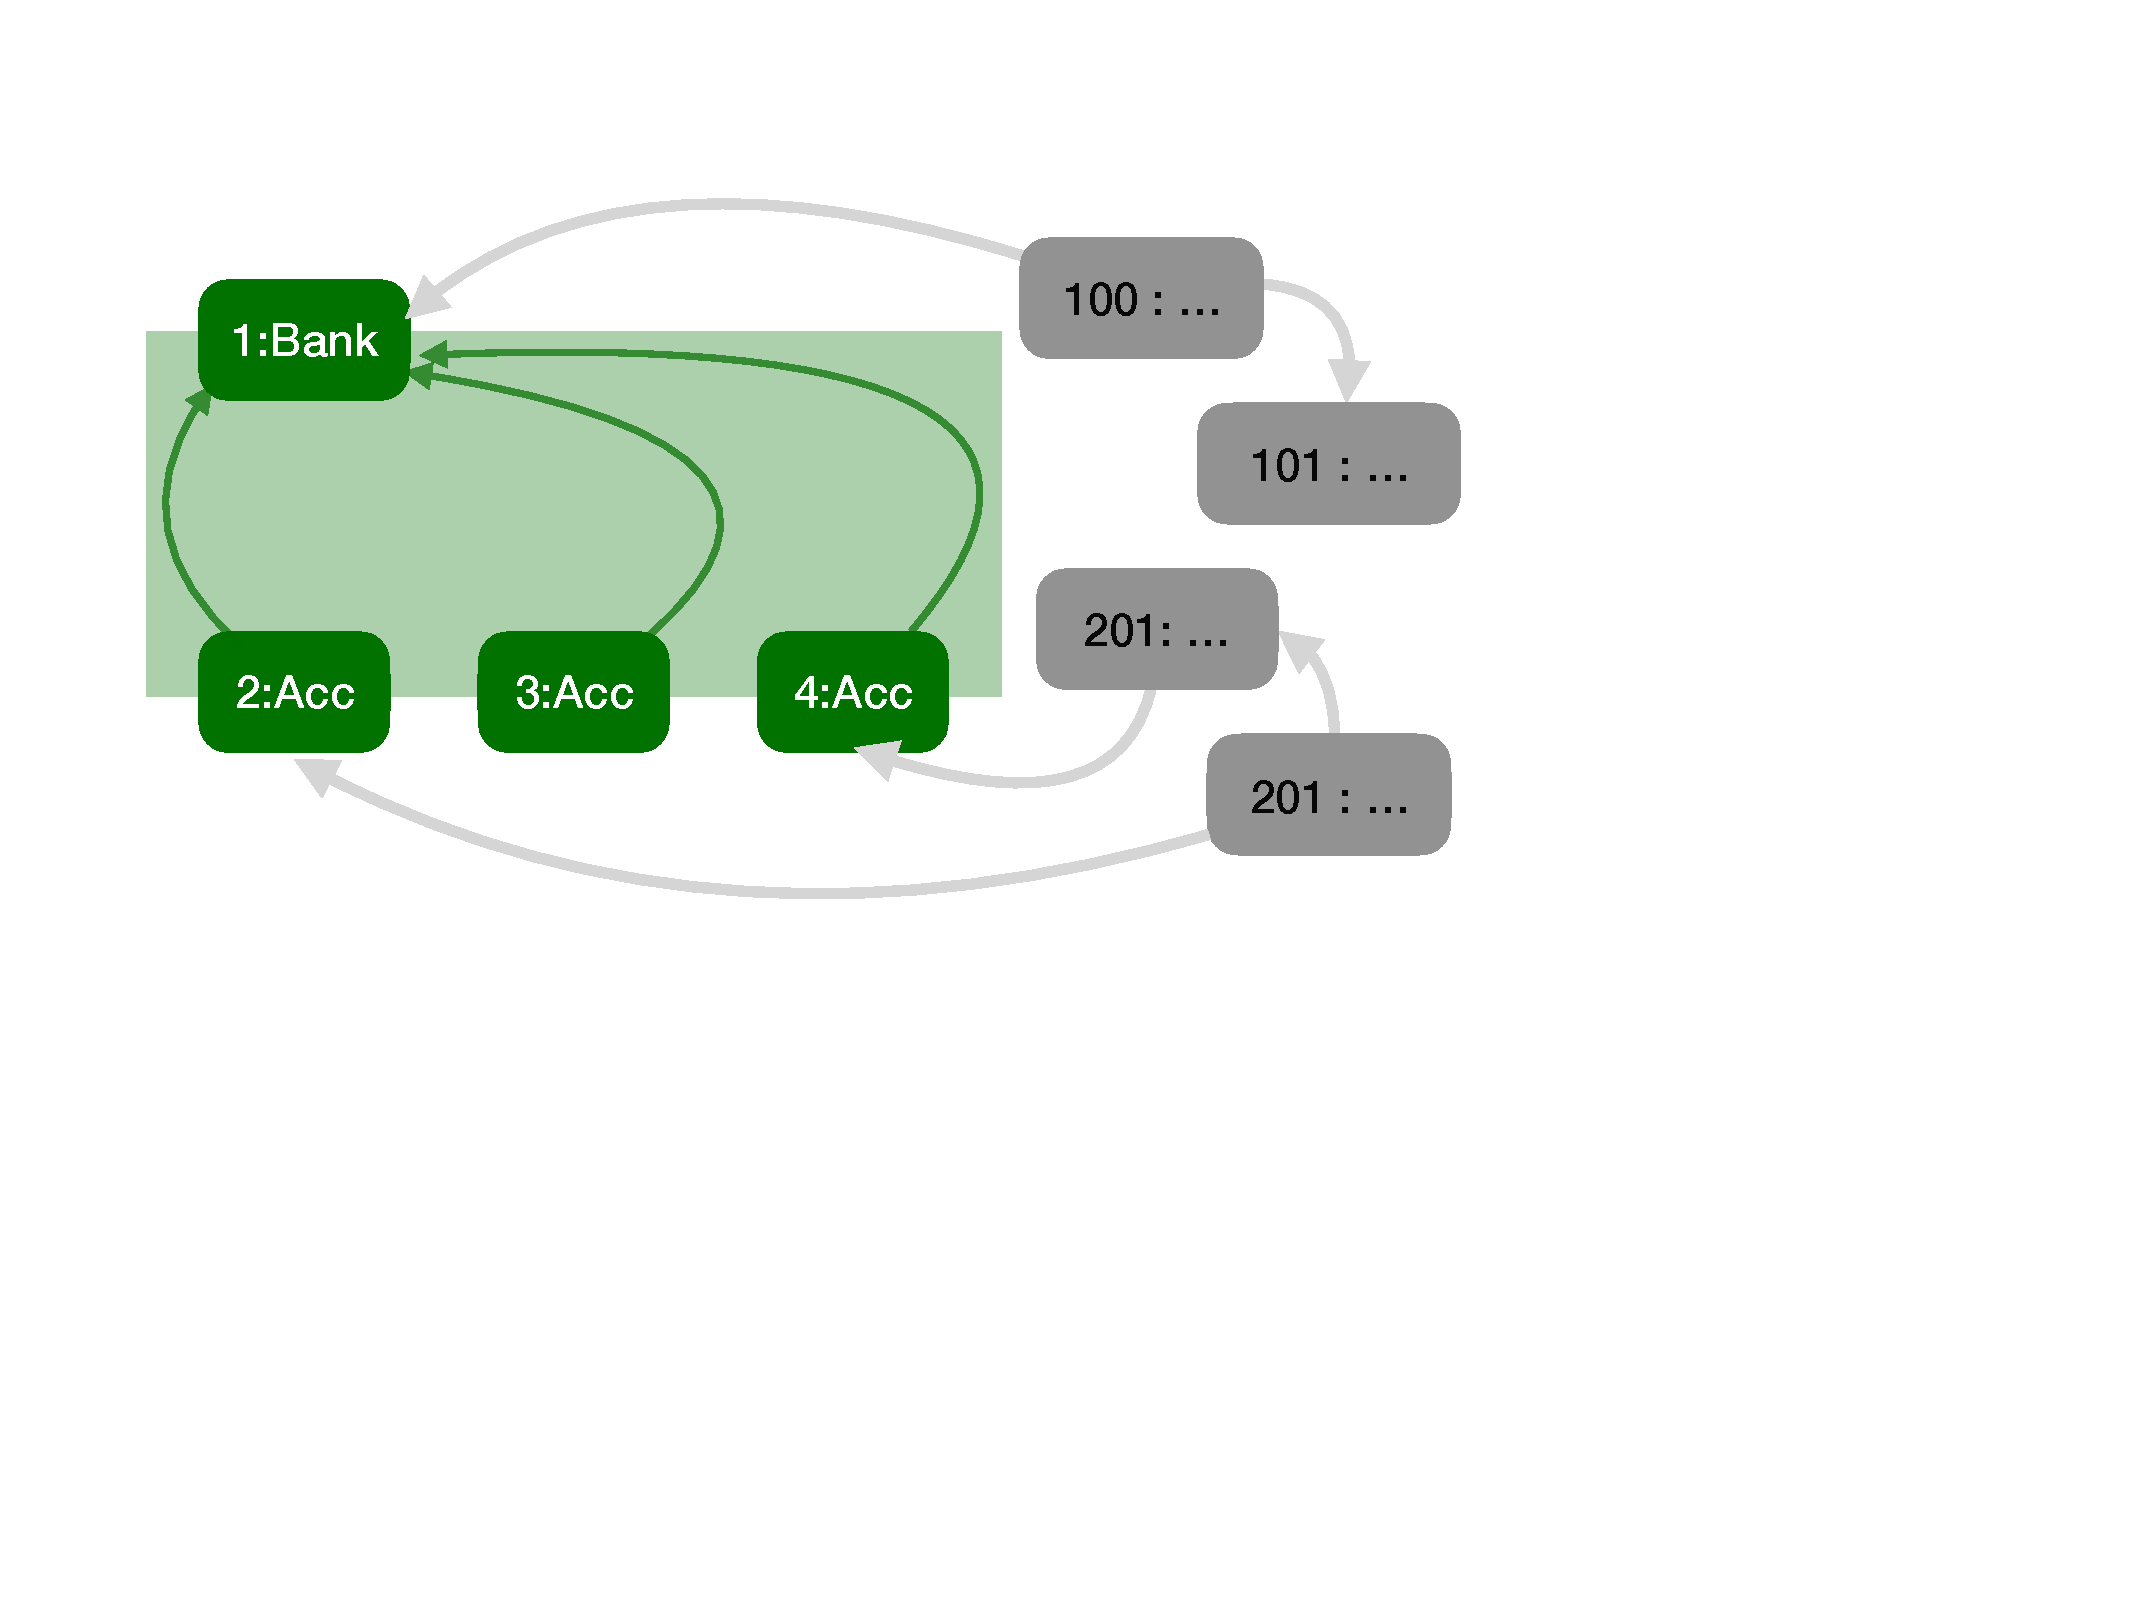
\includegraphics[width=\linewidth, trim=55  330 320 60,clip]{diagrams/BankAccount_version_1.pdf}
   \end{minipage}
 &  
 \begin{minipage}{0.45\textwidth}
 $\sigma_2$\\
  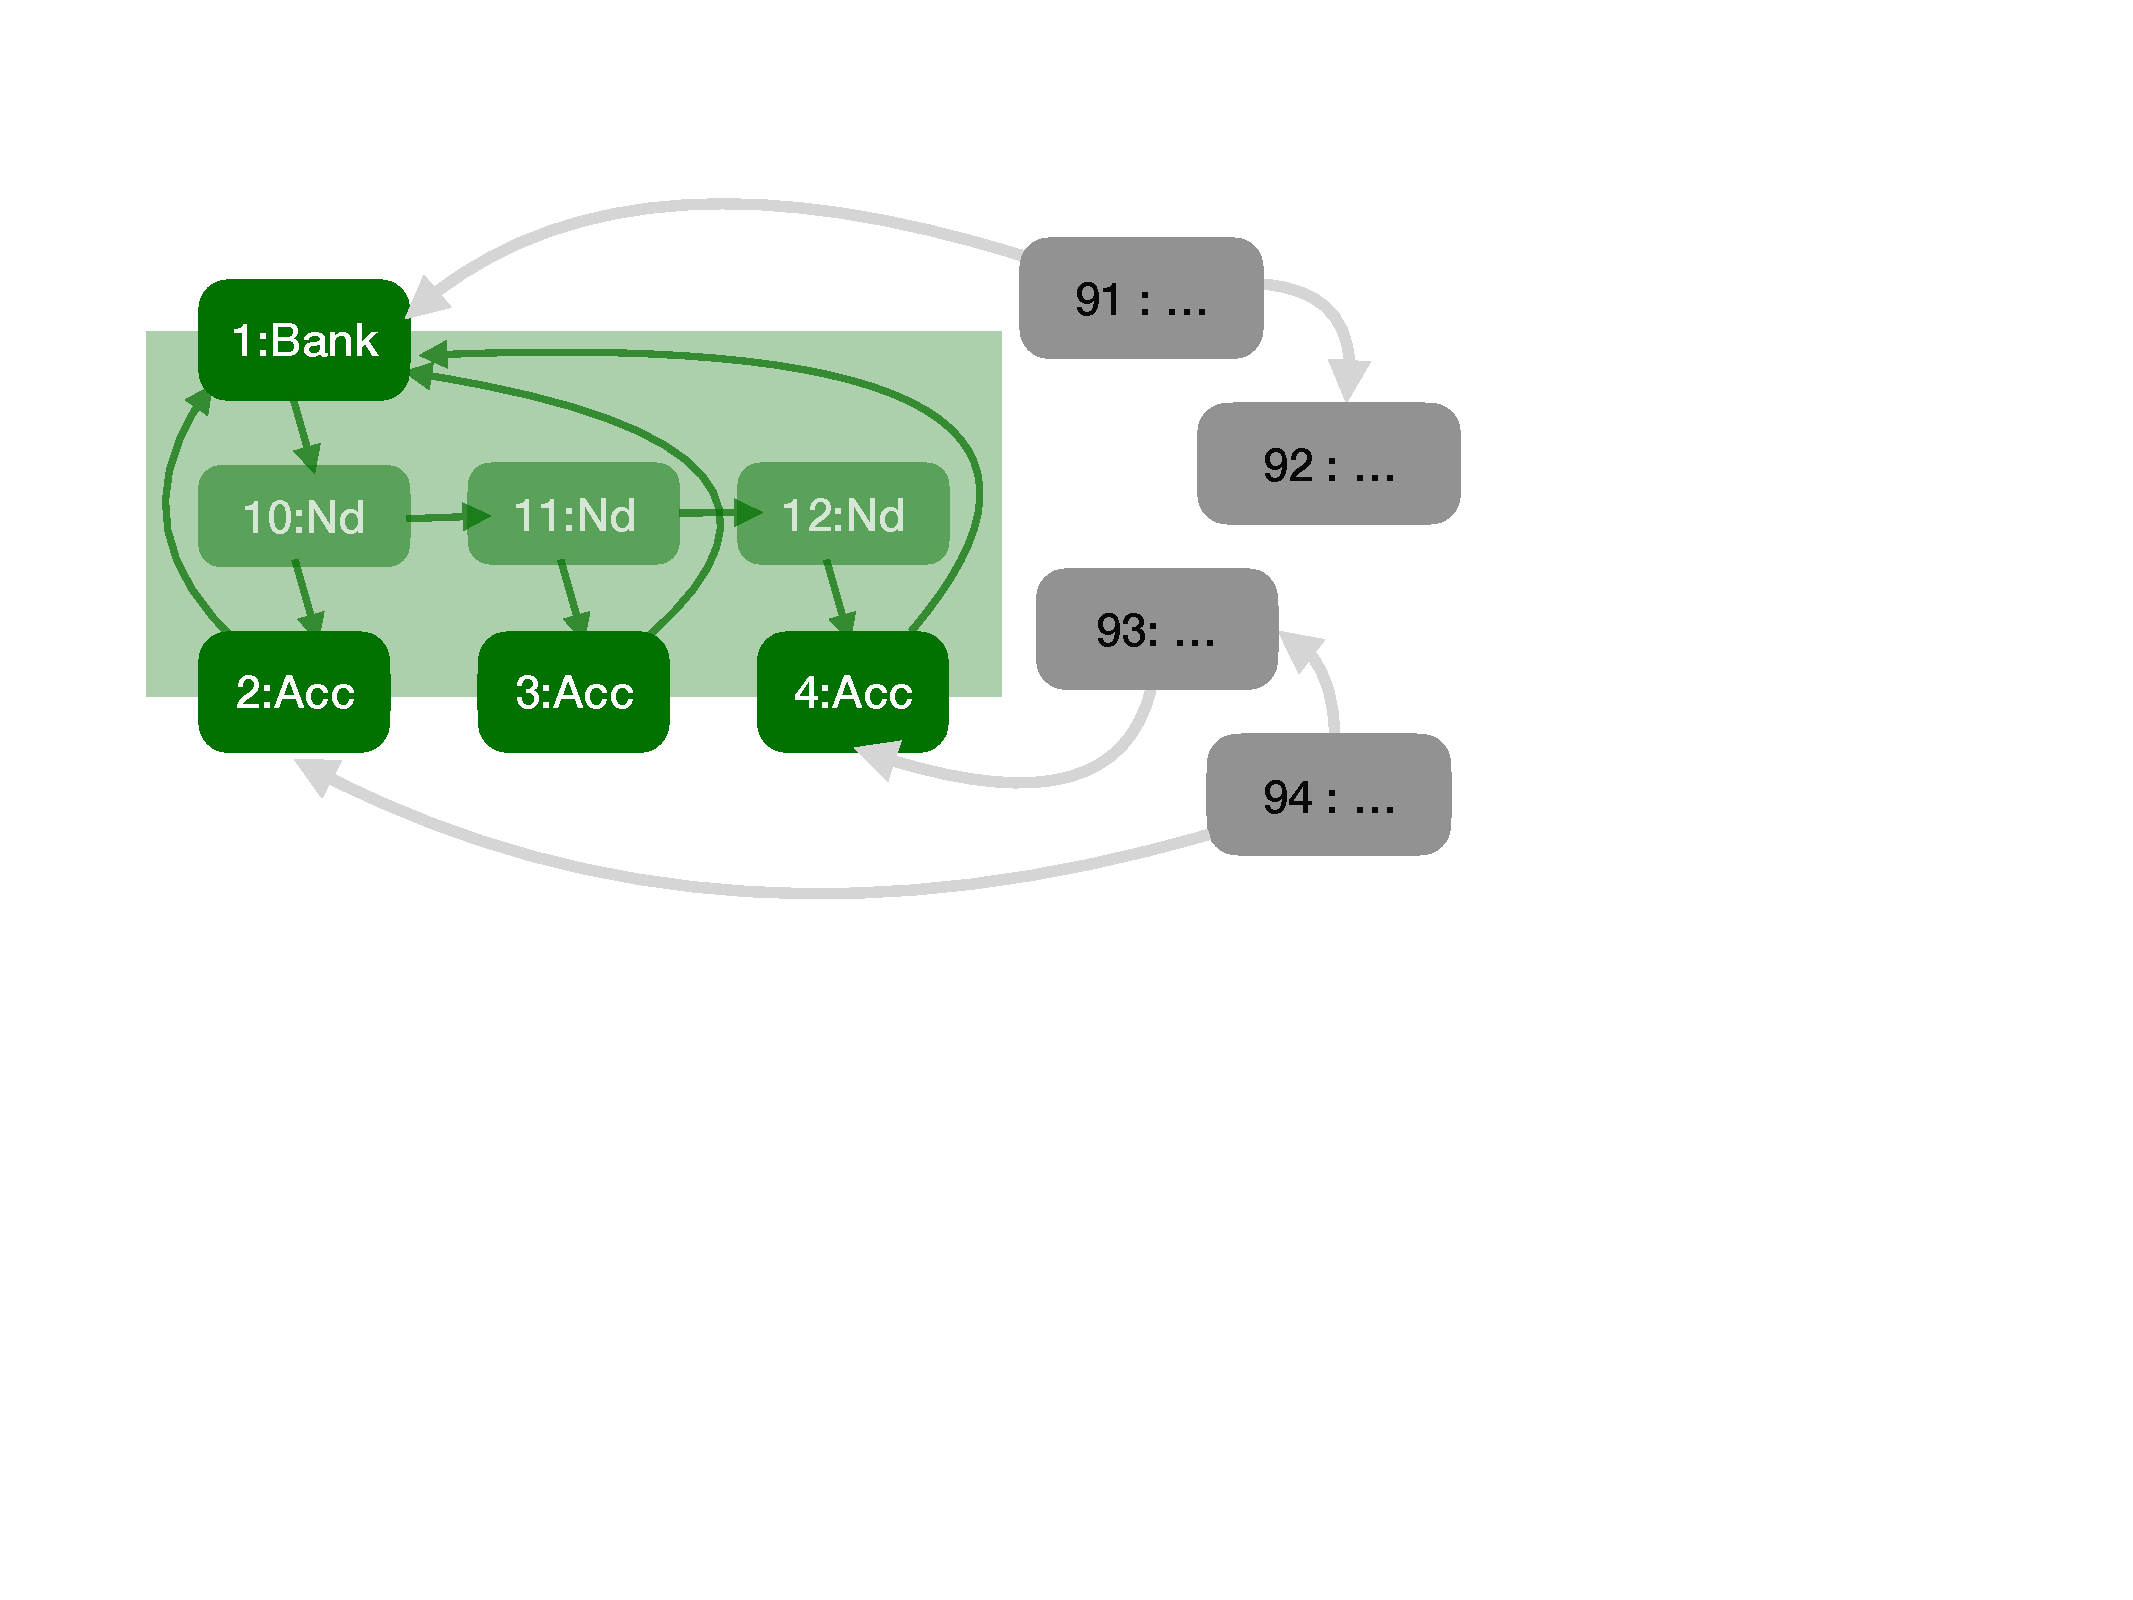
\includegraphics[width=\linewidth, trim=55  330 320 60,clip]{diagrams/BankAccount_version_2.pdf}
   \end{minipage}
\end{tabular}
\end{center}
\caption{Two runtime configurations for the \prg{Bank}/\prg{Account} example. 
}
\Description{Two similar diagrams side-by-side. The left diagram is labelled sigma 1, and the right diagram is labelled sigma 2. Both diagrams contain a green zone, and labelled nodes inside and outside the zone. On the both sides there is a bank with label 1, and 3 accounts with labels 2 through 4 nodes in the zone. All accounts point to their bank, indicating they have a field which accesses the bank. There are also 4 objects outside the zone 91 through 94, with arrows amongst them selves. There is an arrow from object 91 to the bank, from object 93 to the account 4, and object 94 to account 2. On the right there are three additional nodes inside the green zone, nodes 10, 11 and 12. These have arrows to accounts 2, 3, 4, and the next node, respectively. The bank has an arrow to node 10, and these represent the linked list of nodes storing accounts stored within the bank.}
\label{fig:BankAccountDiagrams}
\end{figure}

%\noindent % Not desired after reformatting occurs by LaTeX right now
For the rest, we refer to objects as $\prg{b}_1$, and $\prg{a}_2$--$\prg{a}_4$, and  $\prg{u}_{91}$--$\prg{u}_{94}$, denoting objects \prg{1}, \ \prg{2}--\prg{4},
and   \prg{91}--\prg{94} respectively for both $\sigma_1$ and $\sigma_2$.

\sdparagraph{Classical Assertions} talk about the identity of objects and their 
fields (\ie the heap), as well as referring to local variables (\ie the top frame).
  For example, the assertion  $\ \prg{a}_2.\prg{myBank}$=$\prg{a}_3.\prg{myBank} $, says that
  $\prg{a}_2$ and  $\prg{a}_3$  have the same bank. In fact, this assertion is
  satisfied in both $\sigma_1$ and $\sigma_2$, written formally as\\
  $\strut$ \hspace{1.1cm}  $...,\sigma_1 \ \models \ \prg{a}_2.\prg{myBank}=\prg{a}_3.\prg{myBank}$
  \\
 $\strut$ \hspace{1.1cm}  $...,\sigma_2 \ \models \ \prg{a}_2.\prg{myBank}=\prg{a}_3.\prg{myBank}$.
   
  Note, we elide the module, $M_{BA1}$ or $M_{BA2}$ as ``$...$'', as well as any other requirements to establish an assertion. These are covered in detail in section~\ref{sect:overviewmodel}.
  
  The term \prg{x}:\prg{ClassId} says that \prg{x} is an object of class \prg{ClassId}. For example\\
  $\strut$ \hspace{1.1cm}  $...,\sigma_1 \ \models \ \prg{a}_2.\prg{myBank} : \prg{Bank}$.
  
  We support ghost fields~\cite{ghost,Leavens-etal07}, 
   \eg $\prg{a}_1$.\prg{balance} is a physical field in $\sigma_1$ and a ghost field in $\sigma_2$ since in \prg{MBA2} an \prg{Account} does not store its \prg{balance} (as can be seen in appendix~\ref{Bank:appendix}
Fig.~\ref{fig:BanAccImplV2a}). %\sd{The abstract function %this is a term from the ESOP'06 paper from aboove
 % for \prg{balance}  is defined in  the body of class \prg{Account}}  in \prg{MBA2}  \sd{in the obvious way}.
%
We also support the usual logical connectives, and so, we can express assertions such as \\
$\strut$ \hspace{1.1cm}    $\forall \prg{a}. [ \ \ \prg{a}:\prg{Account} \ \longrightarrow \ \ \prg{a}.\prg{myBank}:\prg{Bank}\ \wedge\  \prg{a}.\prg{balance}\geq 0\ \ ] $ .



\sdparagraph{Permission: Access}
%
Our first holistic assertion, $\CanAccess{\x}{\y}$, asserts that  
object $\x$ has a direct reference to another object $\y$: either one
of $\x$'s fields contains a 
reference to $\y$, or the receiver of the currently executing method is \prg{x}, and \prg{y}
is one of the arguments or is mapped by a local variable. 
For example:\\
 $\strut$ \hspace{1.1cm}  $...,\sigma_0,\sigma_1 \ \models \  \CanAccess{\prg{a}_2}{\prg{b}_1}$
\\
If  $\sigma_1$ 
were executing the method body corresponding to the call ${\prg{a}_2}$.\prg{deposit}\prg{(}${\prg{a}_3}$,\prg{360}\prg{)},  then
we would 
  have\\
 $\strut$ \hspace{1.1cm}  $...,\sigma_1 \ \models \  \CanAccess{\prg{a}_2}{\prg{a}_3}$, \\
 That is, during execution of \prg{deposit}, the object  at   $\prg{a}_2$ has access to the object at $\prg{a}_3$, and could,
  if the method body chose to,  call a method on $\prg{a}_3$ , or  store a reference to $\prg{a}_3$ in its own fields. 
  %  \sophia{ALL: does this clarify why   we define access to take method execution into account?} 
 \sophia{Access} is not symmetric, nor transitive:\\
  $\strut$ \hspace{1.1cm}  $...,\sigma_1 \ \not\models \  \CanAccess{\prg{a}_3}{\prg{a}_2}$, \hspace{0.6cm}\\
  $\strut$ \hspace{1.1cm} 
  $...,\sigma_2 \ \models \  \CanAccess{\prg{a}_2}{\prg{b}_1} \wedge \CanAccess{\prg{b}_1}{\prg{nd}_{10}}$, \hspace{0.6cm}
 %   $\strut$ \hspace{1.1cm}  
 $...,\sigma_2 \ \not\models \  \CanAccess{\prg{a}_2}{\prg{nd}_{10}}$.

%\james{do we really not also need reachable (transitive closure of access)}
%\susan{we don't seem to need transitivity in any of the examples}
%\sophia{We do not want transitivity, our policies where access is in the conclusion would become too weak.}

\paragraph{Control: Calls}
The  assertion $\Calls {\alpha_1} {\m} {\alpha_2} {vs}$ holds 
in configurations where a method on object 
${\alpha_1}$ calls method ${\m}$ on receiver ${\alpha_2}$ with arguments $vs$ --- that is, 
there exists $\x$, $\y$, and $\z_1\dots\z_n = \zs$ in the local variable map that map to $\alpha_1$, $\alpha_2$, and $vs$ 
respectively, and the method call $\y.\m(\zs)$ is made within some method in $\x$.

For example, \\
 $\strut$ \hspace{1.1cm}  $...,\sigma_3 \models \  \Calls {\x}{\prg{deposit}}  {\prg{a}_2} { {\prg{a}_3},\prg{360}}$.\\
 %{{...}} {\prg{a}_2}} {\prg{deposit}} {\prg{(}{\prg{a}_3},\prg{100.00}\prg{)}}$.\\
 means that the receiver in %configuration
 $\sigma_3$ is \x, and that
 $\prg{a}_2.\prg{deposit}{\prg{(}}\prg{a}_3,\prg{360}{\prg{)}}$
 is the next statement to be executed.
 

%% \sdparagraph{Authority --  Changes and Internal/External}\sophia{Is it good to put these together?}
%% The assertion $\Changes{\prg{e}}$  holds when the value of {\prg{e}}
%% in the next configuration is different to the value in the current configuration.
%% For example, if the code being executed in $\sigma_1$ started with $\acc_2.\bal=\acc_2.\bal+\prg{100.00}$, then:\\
%%   $\strut$ \hspace{1.1cm}  $..., \sigma_1 \ \models \  \Changes {\acc_2.\bal}$.\\
%%   Moreover, the assertion $\External {\prg{e}}$ expresses that the object {\prg{e}} does not belong to the module under consideration. 
%%   For example, \\
%% $\strut$ \hspace{1.1cm}  $\M_{AB2}\mkpair ..., \sigma_2 \ \models \ \External{\pu_{92}}$,
%% %$\strut$ 
%% \hspace{1cm}  $\M_{AB2}\mkpair ..., \sigma_2 \ \not\models \ \External{\acc_2}$, \\
%% $\strut$
%%  \hspace{1.1cm}  $\M_{AB2}\mkpair ..., \sigma_2 \ \not\models \ \External{\pb_{1}.\prg{ledger}}$\\
%% Notice the use of the \emph{internal} module, $\M_{AB2}$, needed to judge which objects are internal, and which are external.
 

\sdparagraph{Space: {In}}
The space assertion $\Using{\A}{\SF}$ establishes validity of $\A$ 
 in a configuration  restricted to the 
objects from the set \SF.
% In other words, it restricts the set of objects which may be used to establish property \A. 
For example, 
if  object \prg{94}  is included in $\SF_1$ but not in  $\SF_2$, then we   have\\ 
 $\strut$ \hspace{1.1cm}  $...,\sigma_1 \ \models \ \Using{ (\exists \prg{o}.\,\CanAccess{\prg{o}}{\acc_4})}{\SF_1}$
\\ % $\strut$ \hspace{0.2cm}  
 $\strut$ \hspace{1.1cm}  $...,\sigma_1 \ \not\models \ \Using{ (\exists \prg{o}.\,\CanAccess{\prg{o}}{\acc_4})} {\SF_2}$.\\
 The set \SF\ in the assertion $\Using{\A}{\SF}$  is therefore {\em not} the footprint of   $\A$;
  it is more like the \emph{fuel} \cite{stepindex}  given to establish that assertion. Note that  $...,\sigma \ \models \Using {\A} {\SF}$ does not imply  
  $...,\sigma \ \models \A$  nor does it imply $...,\sigma \ \models \Using {\A} {\SF\cup\SF'}$.
  The other direction of the implication does not hold either.
% \james{would still like  a one sentence motivating/justifying ``with''. Why do we need it}

\sdparagraph{Time: Next, Will, Prev, Was}
We support several operators from temporal
logic: ($\Next \A$, $\Future \A$,  $\Prev \A$, and $\Past \A$) to
talk about the future or the past in one or more \sophia{steps}.
The assertion $\Future \A$ expresses that %after one or more execution steps
$\A$ will hold in one or more steps. For example, 
taking $\sigma_4$ to be similar to  $\sigma_2$, the next statement to be executed 
to be  $\prg{a}_2.\prg{deposit}{\prg{(}}\prg{a}_3,\prg{360}{\prg{)}}$, and 
$\M_{BA2} ...,\sigma_4 \ \models \  \acc_2.\bal=\prg{60}$,  and that
$\M_{BA2} ...,\sigma_4 \ \models \  \acc_4.\bal\geq\prg{360}$,
then\\ 
 $\strut$ \hspace{1.1cm}  $\M_{BA2} ...,\sigma_4 \ \models \ \Future{ {\acc_2.\bal}=\prg{420}}$.\\
The module, $\M_{BA2}$ is needed for looking up the method body of \prg{deposit}.
  
\sdparagraph{Viewpoint: --  External}
%% The assertion $\Changes{\prg{e}}$  holds when the value of {\prg{e}}
%% in the next configuration is different to the value in the current configuration.
%% For example, if the code being executed in $\sigma_1$ started with $\acc_2.\bal=\acc_2.\bal+\prg{100.00}$, then:\\
%%   $\strut$ \hspace{1.1cm}  $..., \sigma_1 \ \models \  \Changes {\acc_2.\bal}$.\\
\Chainmail distinguishes between the internal module $M$, which is the one under consideration, and the external module $M'$, which could contain arbitrary, or even malicious, code. The two modules are specified together as $M\mkpair M'$. The assertion $\External {\prg{x}}$ expresses that the object at \prg{x} does not belong to the internal module.
  For example, \\
$\strut$ \hspace{1.1cm}  $\M_{AB2}\mkpair ...,\sigma_2 \ \models \ \External{\pu_{92}}$,
%$\strut$ 
\hspace{1cm}  $\M_{AB2}\mkpair ...,\sigma_2 \ \not\models \ \External{\acc_2}$, \\
$\strut$
 \hspace{1.1cm}  $\M_{AB2}\mkpair ...,\sigma_2 \ \not\models \ \External{\pb_{1}.\prg{ledger}}$\\

The \emph{internal} module, $\M_{BA2}$, is needed to judge which objects are internal or external.
 
\sdparagraph{Change and Authority:} We have used 
$\Changes {...}$ 
in our \Chainmail assertions in section~\ref{sect:motivate:Bank}, as in
 $\Changes  {\acc.\prg{balance}}$. Assertions that talk about change, or give conditions for change
to happen are fundamental for security; the ability to cause change is called \emph{authority} in \cite{MillerPhD}. 
We can encode change using the other features of \Chainmail, namely, for any expression \e: 

$\strut$ \hspace{1.1cm}
$\Changes {\e}$\  \ $\equiv$\ \ $\exists v. [\ \e=v \wedge \Next {\neg ( \prg{e}=v)}\ ]$.\\
and similarly for assertions.
%
%\kjx{wishes we could do:\\
%$\strut$ \hspace{1.1cm}
%$\Changes {\e}$\  \ $\equiv$\ \ $\neg (\prg{e} \prg{==} \Next
%{\prg{e}}) $\\
%but can't because $\Next{A}$ only applies to assertions.}




%\sophia{The observer pattern example is very nice, but unfortunately we cannot use it, because the
%calls are internal, and therefore not visible in the current system.}
%For example, a part of the observer pattern is that when
%a subject is notified of a change, then the observer must
%be told to update itself.    We can write this from the
%subject's perspective, looking forwards:
%
%\begin{lstlisting}
%  Call(_,subject,notify,_) --> Will(Call(subject,observer,update,_))
%\end{lstlisting}
%
%\noindent meaning that once notify is called on a subejct, then its
%observer will be updated sometime in the future.  We can write a very
%similar specification for an observer, looking backwards.
%
%\begin{lstlisting}
%  Call(subject,observer,update,_) --> Was(Call(_,subject,notify,_))
%\end{lstlisting}
%
%\noindent meaning that if a subject updates an observer, that subject
%have been notified sometime previously. We could tighten each
%specifaction, so that the update must immediately follow the
%notification, by replacing $\Future \A$ or $\Past \A$ with 
%$\Next \A$ or $\Prev \A$.

\sdparagraph{Putting these together} We now look at some composite assertions which use  
 several features from above. For example, the assertion below 
says that if the statement to be executed is   $\acc_2.\prg{deposit}\prg{(}\acc_3,\prg{60}\prg{)}$,
then the balance of $\acc_2$ will eventually change:\\

\vspace*{-1mm}
\noindent $\M_{BA2}\mkpair ...,\sigma_2 \ \models \ {\Calls {\_}   {\prg{deposit}} {\acc_2} {\acc_3,\prg{60}} } \longrightarrow {\Future{ \Changes {\acc_2.\bal}}}$.

\vspace{.2cm}
 
Now look deeper into space assertions, $\Using{\A}{\SF}$, which
allow us to characterise the set of objects which have authority over
certain effects (here $\A$). In particular,  the assertion   $\Using
{\Future {\A}} {\SF}$  requires that $\A$ will hold in
the future if only the objects in \SF\ are considered.
Knowing who has, and who has not, authority over properties or data is a fundamental concern of robustness
\cite{MillerPhD}. Notice that the authority is a set, rather than a single object: quite often it takes \emph{several objects in concert}
 to achieve an effect.


Consider assertions (2) and (3) from the previous section. They
  both have the form ``$\Future {\Using {\A} {\SF}}\ \longrightarrow P(\SF)$'',
  where $P$ is some property over a set. These \sophia{assertions} say that if
  ever in the future $\A$ becomes valid, and if the objects involved
  in making $\A$ valid are included in $\SF$, then in the current configuration $\SF$ must satisfy
  $P$. Such assertions can be used to restrict whether $\A$ will
  become valid. If we have some execution which only involves objects which do not satisfy $P$, then we know that the execution will not ever make $\A$ valid.

%\susan{I don't know where m and m2 come from. We haven't seen them up to now and I don't  see why they are needed in this story.}

%%\vspace{.2in} 
%\sophia{While
%many  individual
%features of \Chainmail can  be found also in other work, we
%%claim that their  combination as well as
%%their application in the specification of open systems are novel.
%argue that their power and novelty for specifying open systems lies in their careful
%  combination}

\sdparagraph{In summary,} in addition to classical 
logical connectors and classical assertions over the contents of the heap and the stack, 
our holistic assertions draw from some concepts from object capabilities
($\CanAccess{\_}{\_}$  for  permission; $\Calls {\_} {\_} {\_} {\_}$ and  $\Changes{\_}$ for
authority) 
as well as temporal logic ($\Future \A$, $\Past \A$ and friends), and the relation of
our spatial connective ($\Using{\A}{S}$)  with ownership and effect
systems \cite{typeEffect,ownalias,ownEncaps}.

The next two sections  discuss the semantics of \Chainmail. Section \ref{sect:formal}
contains an overview of the formal model and section \ref{sect:assertions} focuses on the most important part of \Chainmail : assertions.

%its most important aspect being assertions, whose semantics are in section  \ref{sect:assertions}.

%\james{somewhere, should we say something like: the goal is
%  to allow wholistic specifations with as extra little machinery as
%  possible over a basic Hoare language}.




\section{Overview of the \Chainmail\  formal model}
\label{sect:overviewmodel}
%\section{Overview of the \Chainmail\  formal model}
% \subsection{The Open World}

\kjx{Can we have a better title? is this style of modelling the adversary claimed contribution of the paper that we should claim explicitly?  IF so the title should highlight that claim.}

Having outlined the ingredients of our holistic specification
language, the next question to ask is: When does a module $\M$ satisfy
an holistic assertion $\A$?  More formally: when does
%
%\sd{So, the question about modules satisfying assertions put formally is,} when does  \\
$~ \strut  \hspace{1.3in}\ \M \models \A$ \\
hold? \kjx{do we really want M modles A on a line on its own?}

  
Our answer has to reflect the fact that we are dealing with an 
\emph{open  world},  where  $\M$, our module, may be
linked with \textit{arbitrary untrusted code}.
Modules are repositories of code, so we adopt the common formalisation 
of modules as  mappings from
class identifiers to class definitions.
%
%% \sd{Note that we use the term \emph{module} to talk about repositories of code; in this work modules are mappings from
%% class identifiers to class definitions.}
%
%
To model the open world, we consider
 pairs of modules, 
$\M \mkpair {\M'}$,  where $\M$ is the module 
whose code is supposed to satisfy the assertion,
and $\M'$  is  another % wused to say \textit{any}  -- but why?
 module which exercises
the functionality of $\M$. We call our module $\M$ the {\em internal} module, and
 $\M'$ the {\em external} module, which represents potential
 attackers or adversaries.
%or {\em potentially adversarial} module. 
    
We can now answer the question: $\M \models \A$ 
 holds if for all further, {\em potentially adversarial}, modules $\M'$ and in  all runtime configurations $\sigma$ which may be observed as arising from the  execution of the code of $\M$ combined with that of $\M'$, the assertion $\A$ is satisfied. More formally, we define:\\
$~ \strut  \hspace{1.3in} \M \models \A \ \ \  \ \ \ \ \ \mbox{
if               } \ \ \  \ \ \  \  \forall \M'.\forall \sigma\in\Arising
{\M \mkpair  {\M'}}. [\ \M \mkpair  {\M'},\sigma \models \A\ ]$.  \\
Module $\M'$ represents all possible clients of {\M}; and as it is arbitrarily chosen, it reflects the open world nature of our specifications.%\sdcomment

%% \sophia{Is is sentence superfluous now?.}
%% \sophia{In contrast to what we said on Friday's conf call we do not need to put any restrictions
%% on $\M'$ -- not even disjointness is required.}
%% \kjx{OK so in the \textbf{next iteration} we can just replace M;M' with a ' operator applied to any module\ldots}

The judgement $\M \mkpair  {\M'},\sigma \models \A$ means that  
assertion $\A$ is satisfied by  $\M \mkpair  {\M'}$ and $\sigma$.  
As in traditional specification languages \cite{Leavens-etal07,Meyer92}, satisfaction is judged 
in the context of  runtime configuration $\sigma$; but in addition, it is judged in the context of the internal and external modules.
We need the modules, because temporal assertions may
talk about future configurations: the modules contain the code necessary to reach those configurations.

Our distinction between internal and external modules offers two other advantages.
\kjx{is this distinction a claimed contribution?}
First, 
\Chainmail\ includes the ``$\External{\prg{o}}$'' assertion to require
that an object belongs to the external module, as in the Bank
Account's assertion (2)and (3) in
section~\ref{sect:motivate:Bank}. Second, we adopt a version of
visible states semantics \cite{visible-state-semantics}, treating all
executions within a module as atomic.
We only record runtime configurations which are {\em external}
 to module $\M$, \ie those where the
 executing object (\ie the current receiver) comes from module $\M'$.
 Program execution is
 a judgment of the form\\
 $~ \strut  \hspace{1.3in}    \M \mkpair  {\M'},\sigma \leadsto \sigma'$\\  
 where we ignore all intermediate steps
 whose receivers are internal to $\M$. 
Similarly, when considering $\Arising {\M \mkpair  {\M'}}$, \ie the configurations arising from 
executions in $\M \mkpair  {\M'}$, we can take method bodies defined in $\M$ or in $\M'$, but we will only consider the runtime 
configurations which are external to $\M$.

%\sd{Therefore, the pair $\M \mkpair  {\M'}$ is different than the concatenation of the two modules}
%In  that sense, our approach is similar to that of visible states semantics, without, however the need to consider issues
%around different objects of the same class or re-entrancy.

\kjx{if this is about the internal/external distinction, I'd move the
following to section 6?, someoone else should check}

\sd{As a notational convenience, we keep the code to be executed as a component of the runtime configuration.
Thus, $\sigma$ consists of a stack of frames and a heap, and each frame consists of a variable map and a continuation.
The variable map is a mapping from variables to addresses or to set of addresses -- the latter are needed to
deal with assertions which quantify over footprints, as \eg (1) and (2) from section \ref{sect:motivate:Bank}.}


\sd{To give meaning to assertions with footprint restrictions such as \eg $\Using {\A} {\prg{S}}$ ,we define  restrictions on the
configuration. Thus $\sigma\!\!\downarrow_{\sigma(\prg{S})}$ is the same as $\sigma$ but with the domain of the heap restricted
to the addresses from $\sigma(\prg{S})$. And then we define\\
  $~ \strut  \hspace{1.3in} \M \mkpair  {\M'},\sigma  \models\Using {\A} {\prg{S}}$\ \ \ \ \ if \ \ \ \  \  $\M \mkpair  {\M'},\sigma\!\!\downarrow_{\sigma(\prg{S})}  \models {\A}$}
  
\sd{The meaning of assertions therefore may depend on the variable map, eg \prg{x} may be pointing to a different 
object in .... TODO
The treatment of time in combination with the fact that the meaing od assertions TODO}




\section{ Assertions}
\label{sect:assertions}

\Chainmail assertions (details in appendix \ref{sect:standard}) consist of (pure) expressions \e, comparisons between expressions, classical
assertions about the contents of heap and stack, the usual logical
connectives, as well as our holistic concepts.
In this section we focus on the novel,
 holistic, features of \Chainmail (permission, control, time, space, and viewpoint),
as well as our wish to support some form of recursion while keeping the logic of assertions classical.
% SD I removed the belowas it is no longer true here. % don't understand what you mean so i have deleted the next paragraph
%\sdN{Expressions include variables, field lookup, and the execution of (pure) ghost methods. 
%This  supports recursion at the level of expressions; therefore, the value of  an expression  may be
% undefined (either because of infinite recursion, or because the expression accessed undefined fields or variables). 
 %Assertions of the form   $\e$=$\e'$ are satisfied only if both $\e$ and $\e'$ are defined. Because we do not support 
% recursion at the level of assertions, assertions form a classical logic (\eg $\A \vee \neg\A$ is a tautology)
%}
%Assertions support the comparison of expressions, and the usual logical connectives
%(Appendix, section \ref{sect:standard}), as well as the usual connectives discussed below.
%We now define the syntax and semantics of expressions and holistic assertions.
%\sd{The novel, holistic, features of \Chainmail (permission, control, time, space, and viewpoint),
%as well as our wish to support some form of recursion while keeping the logic of assertions classical,  introduced 
%challenges, which we discuss in this section.}

\subsection{Syntax and Semantics}
 
We now define the syntax and semantics of expressions and holistic assertions.
\sd{The novel, holistic, features of \Chainmail (permission, control, time, space, and viewpoint),
as well as our wish to support some form of recursion while keeping the logic of assertions classical,  introduced 
challenges, which we discuss in this section.}

 \subsection{Syntax of Assertions}
 


\begin{definition}[Assertions]  \sd{Assertions consist of (pure) expressions \e, classical assertions about the contents of heap/stack, the usual logical  connectives, as well as our holistic concepts.}
\label{def:assertions}


 $\begin{array}{lcl}
  ~  \\
 \SE  &\BBC&    \kwN{true}   ~\SOR~  \kwN{false}   ~\SOR~  \kwN{null}  ~\SOR~  \x  \   ~\SOR~  
     \   \SE=\SE    ~\SOR~ \kwN{if}\, \SE\,   \kwN{then}\,  \SE\,    \kwN{else}\, \SE    ~\SOR~  \SE.\f\lp\ \SE^* \ \rp\\
     \\
 \A &\ \BBC   &   \SE \   \mid \  \SE=\SE  \mid \   \SE:\prg{ClassId}  \ \mid \
    \SE\in\prg{S}   \mid  \  \\
    &
  &  \A \rightarrow \A  \ \mid\  \     \A \wedge \A  \ \mid\  \  \A \vee \A  \ \mid\  \ \neg A   \ \mid \ \\
  & &  \forall \x.\A  \ \mid \  \forall \prg{S}:SET.\A  \ \mid  \  \exists \x.\A  \ \mid \  \exists \prg{S}:SET.\A  \  \ \mid\   \\
 &    &  \CanAccess x y %\ \mid\  \ \Changes e 
           \ \mid\  \Calls {\prg{x}}  {\prg{m}} {\prg{x}}  {\prg{x}^*}\\          
% &    &  \kjx{\CanAccess x y \ \mid\  \ \Changes e 
%           \ \mid\  \Calls {\prg{x}}  {\prg{m}} {\prg{x}}  {\prg{x}^*} }\\
&    &  \Next \A  \ \mid \   \Future \A \ \mid \  \Prev \A   \ \mid \ \Past \A \ \mid \\  
 &    &        \Using \SF  \A  \ \mid \  \External \x     \\
% &    &   \kjx{\Using \SF  \A  \ \mid \  \External \x \ \mid \ \prg{x} \obeys \prg{S} }  \\
 \\
 \x, \f, \m &\BBC&  \prg{Identifier}  ~ \\
\end{array}$
\end{definition}
%% \footnote{
%% The operators $\wedge$, $\vee$,  $\neg$ and $\forall$  could have been
%% defined  through the usual shorthands, \eg, $\neg \A$ is short for
%% $\A \rightarrow \ff$ \etc, but here we give full definitions
%% instead\kjx{can we just cut this please?}}

\jm{
\begin{definition}[Assertions]  \sd{Assertions consist of (pure) expressions \e, classical assertions about the contents of heap/stack, the usual logical  connectives, as well as our holistic concepts.}
\label{def:assertions}
 \[
 \begin{array}{lcl}
  ~  \\
 \prg{v}  &\BBC&    \kwN{true}   ~\SOR~  \kwN{false}   ~\SOR~  \kwN{null}  ~\SOR~  \alpha  \\
  ~  \\
 \SE  &\BBC&    \prg{v}\ ~\SOR~ \SE=\SE    ~\SOR~ \kwN{if}\, \SE\,   \kwN{then}\,  \SE\,    \kwN{else}\, \SE    ~\SOR~  \SE.\f\lp\ \SE^* \ \rp\\
     \\
 \A &\ \BBC   &   \SE \   \mid \  \SE=\SE  \mid \   \SE:\prg{ClassId}  \ \mid \
    \SE\in\prg{S}   \mid  \  \\
    &
  &  \A \rightarrow \A  \ \mid\  \     \A \wedge \A  \ \mid\  \  \A \vee \A  \ \mid\  \ \neg A   \ \mid \ \\
  & &  \forall \alpha.\A  \ \mid \  \forall \prg{S}:SET.\A  \ \mid  \  \exists \alpha.\A  \ \mid \  \exists \prg{S}:SET.\A  \  \ \mid\ \forall \m.\A \ \mid\ \exists \m. \A \ \mid \\
 &    &  \CanAccess {\alpha_1} {\alpha_2} %\ \mid\  \ \Changes e 
           \ \mid\  \Calls {\alpha_1}  {\prg{m}} {\alpha_2}  {\prg{v}^*}\\          
 &    &  \CanAccess x y \ \mid\  \ \Changes e 
           \ \mid\  \Calls {\prg{x}}  {\prg{m}} {\prg{x}}  {\prg{x}^*} \\
&    &  \Next \A  \ \mid \   \Future \A \ \mid \  \Prev \A   \ \mid \ \Past \A \ \mid \\  
 &    &        \Using \SF  \A  \ \mid \  \External \alpha \ \mid\ \prg{name}\langle \alpha, \x \rangle \ \mid \\
 &    &   \Using \SF  \A  \ \mid \  \External \x \ % \mid \ \\ \prg{x} \obeys \prg{S}  \\
 \\
 \x, \f, \m &\BBC&  \prg{Identifier}  ~ \\
\end{array}
\]
\end{definition}}
 
Expressions support calls with parameters  ($\e.\f(\e^*)$); these are calls to ghostfield
functions. This  supports recursion at the level of expressions; therefore, the value of  an expression  may be
undefined (either because of infinite recursion, or because the expression accessed undefined fields or variables). 
Assertions of the form   $\e$=$\e'$ are satisfied only if both $\e$ and $\e'$ are defined. Because we do not support 
recursion at the level of assertions, assertions from a classical logic (\eg $\A \vee \neg\A$ is a tautology).
 
We will discuss evaluation of expressions in section \ref{sect:expressions}, standard assertions about heap/stack and logical
 connectives in \ref{sect:standard}. 
 \sophia{We have discussed  the treatment of  permission, control, space, and viewpoint  in 
the main text in the  Definitions 3-7  in section \ref{sect:pcsv} %HARD
the treatment of time in  Definitions 8,9 in the main text, section \ref{sect:time},
We will discuss properties of assertions in Lemmas \ref{lemma:classic}-\ref{lemma:classic:two}.}
 The judgement $\M\mkpair \M', \sigma_0 \ldots  \sigma  \models \A$ expresses that $\A$ holds in  $\M\mkpair \M'$ and $\sigma$, and 
while $\M\mkpair \M', \sigma_0 \ldots   \sigma  \not\models \A$  expresses that $\A$ does not hold  in  $\M\mkpair \M'$ and $\sigma$.
 
\subsection{Values of Expressions}
\label{sect:expressions}

The value  of  an expression  is described through judgment $ \M,\, \sigma, \SE \ \hookrightarrow\  v$,
defined in  Figure \ref{fig:ValueSimpleExpressions}.
We use the configuration, $\sigma$, to read the contents of the top stack frame
% value of variables defined in the stack frame
(rule ${\sf {Var\_Val}}$) or the contents of the heap (rule
${\sf {Field\_Heap\_Val}}$). We use the module, \M, to find the  ghost field declaration corresponding to the
ghost field being used. 


The treatment of fields and ghost fields is described in rules ${\sf {Field\_Heap\_Val}}$,\\  ${\sf {Field\_Ghost\_Val}}$ and 
${\sf {Field\_Ghost\_Val2}}$.  If the field \f~ exists in the heap, then its value is returned (${\sf {Field\_Heap\_Val}}$). 
Ghost field reads, on the other hand, have the form $\e_0.\f(\e_1,...\e_n)$, and their value is
described in rule ${\sf {Field\_Ghost\_Val}}$:
%
The lookup function $\mathcal G$  (defined in the obvious way in the Appendix, Def.\ref{def:lookup})
returns the expression constituting the body for that ghost field, as defined in the class of $\e_0$.
We return  that expression
evaluated in a configuration where the formal parameters have been substituted by the values of the actual
parameters.

Ghost fields support recursive definitions. For example, imagine a module $\M_A$ with
a class \prg{Node} which has a field called \prg{next}, and which 
had a ghost field \prg{last}, which finds  the last \prg{Node} in a sequence
and is defined recursively as \\
$~ \strut \hspace{.1cm}$ \ \ \ \prg{if}\ \ \prg{this.next}=\prg{null}\  \prg{then} \ \prg{this} \ \prg{else} \ \prg{this.next.last},\\
and another ghost field \prg{acyclic}, which expresses that a sequence is acyclic,
defined recursively as \\
$~ \strut \hspace{.1cm}$ \ \ \ \prg{if}\ \ \prg{this.next}=\prg{null}\  \prg{then} \ \prg{true} \ \prg{else} \ \prg{this.next.acyclic}.

The relation $ \hookrightarrow$ is partial. 
For example, assume   a configuration
$\sigma_A$ where
\prg{acyc} points to a \prg{Node} whose field \prg{next} has value \prg{null}, and   
\prg{cyc} points to a \prg{Node} whose field \prg{next} has the same value as \prg{cyc}. Then,   
$\M_A,\sigma_A,\,\prg{acyc.acyclic}  \ \hookrightarrow\  \prg{true}$, but we would have no value for 
$\M_A,\sigma_A,\, \prg{cyc.last}  \ \hookrightarrow\  ...$, nor for
$\M_A,\sigma_A,\, \prg{cyc.acyclic}  \ \hookrightarrow\  ...$.

Notice also that for an expression of the form  
\prg{\e.\f}, both ${\sf {Field\_Heap\_Val}}$ and ${\sf {Field\_Ghost\_Val2}}$ could be applicable: rule ${\sf {Field\_Heap\_Val}}$
will be applied if \prg{f} is a field of the object at \prg{e}, while rule ${\sf {Field\_Ghost\_Val}}$
will be applied if \prg{f} is a ghost field of the object at \prg{e}. We expect the set of fields and ghost fields in a 
given class to be disjoint.
This allows a specification to be agnostic over whether a field is a physical field or just ghost information.
For example, assertions (1) and (2) from  section  \ref{sect:motivate:Bank}
 talk about the \prg{balance} of an \prg{Account}. 
In module $\M_{BA1}$ (Appendix~\ref{Bank:appendix}), where we keep the balances in the account objects, this is a physical field. 
In $\M_{BA2}$ (also in Appendix~\ref{Bank:appendix}), where we keep the
balances in a ledger, this is ghost information.  
 

\begin{figure*}
{
$\begin{array}{l}
\begin{array}{llll}
\inferenceruleN {True\_Val} {
}
{
 \M,\, \sigma, \kwN{true} \ \hookrightarrow\  \kwN{true}
}
& 
\inferenceruleN {False\_Val} {
}
{
 \M,\, \sigma, \kwN{false} \ \hookrightarrow\  \kwN{false}
}
&
\inferenceruleN  {Null\_Val} {
}
{
 \M,\, \sigma, \kwN{null} \ \hookrightarrow\  \kwN{null}
}
&
\inferenceruleN {\mrrz{Addr\_Val}%{Had to switch old \textit{Var_Val} rule for \textit{Addr_Val}}
} {
\alpha : \text{Address}
}
{
 \M,\,  \sigma, \alpha \ \hookrightarrow\   \alpha
}
\end{array}
\\ \\
\begin{array}{lll}
\begin{array}{l}
\inferenceruleNM{Field\_Heap\_Val} {
 \M,\,  \sigma, \SE \ \hookrightarrow\   \alpha \hspace{1.5cm} 
 \sigma(\alpha,\f)=v
}
{
 \M,\, \sigma, \SE.\f  \ \hookrightarrow\   v
}
\\
\\
\inferenceruleNM{Field\_Ghost\_Val2} {
 \M,\, \sigma, \SE.\f \lp \rp \ \hookrightarrow\   v
}
{
 \M,\, \sigma, \SE.\f   \ \hookrightarrow\   v
}
\end{array}
& &
\inferenceruleNM{Field\_Ghost\_Val}
{
~ \\
 \M,\, \sigma, \SE_0   \ \hookrightarrow\  \alpha
\\
 \M,\, \sigma, \SE_i  \ \hookrightarrow\   v_i\ \ \ \ i\in\{1..n\}
 \\
{\mathcal{G}}
(\M, {\ClassOf {\alpha} {\sigma}}, {\f}) \  =  
\ \f\lp \p_1, \ldots \p_n \rp \lb\ \SE \ \rb
  \\
  \M,\,\sigma[\p_1\mapsto v_1, .... \p_n\mapsto v_n], \SE    \hookrightarrow_{\SAF}\   v 
 }
{
 \M,\,  \sigma, \ \SE_0.\f \lp \SE_1,....\SE_n\rp \hookrightarrow   \ v
}
\\ \\
\inferenceruleNM{If\_True\_Val} 
{
 \M,\,  \sigma, \SE \ \hookrightarrow\   \prg{true}  \\
   \M,\,  \sigma, \SE_1 \ \hookrightarrow\   v  
}
{
 \M,\, \sigma, \kwN{if}\ \SE\  \kwN{then} \ \SE_1 \ \kwN{else} \ \SE_2\  \hookrightarrow  \ v
}
& &
\inferenceruleNM {If\_False\_Val} 
{
 \M,\,  \sigma, \SE \ \hookrightarrow\   \prg{false}  \\
   \M,\,  \sigma, \SE_2 \ \hookrightarrow\   v  }
{
 \M,\, \sigma, \kwN{if}\ \SE\  \kwN{then} \ \SE_1 \ \kwN{else} \ \SE_2\  \hookrightarrow\  v
}
\\ \\ 
\inferenceruleNM {Equals\_True\_Val} 
{
 \M,\,  \sigma, \SE_1 \ \hookrightarrow\    v \\
   \M,\,  \sigma, \SE_2 \ \hookrightarrow\     v 
}
{
 \M,\, \sigma, \SE_1 =  \SE_2 \hookrightarrow \prg{true}
}
& &
\inferenceruleNM {Equals\_False\_Val} 
{
 \M,\,  \sigma, \SE_1 \ \hookrightarrow\    v \\
   \M,\,  \sigma, \SE_2 \ \hookrightarrow\     v' \hspace{2cm}  v\neq v'
}
{
 \M,\, \sigma, \SE_1 =  \SE_2 \hookrightarrow \ \prg{false}
}
\end{array}
\end{array}
$}
\caption{Value of  Expressions}
\label{fig:ValueSimpleExpressions}
\end{figure*}
\subsection{Satisfaction of Assertions - standard}
\label{sect:standard}
\sd{
We now define the semantics of assertions involving expressions, the heap/stack, and logical connectives.
The semantics are unsurprising, except, perhaps the relation between validity of assertions and the values of
expressions.
}


 \begin{definition}[Interpretations for simple expressions]

\mrr[For a runtime configuration, $\sigma$,    variables $\x$ or \SF, we define its interpretation as follows:]{Is it still necessary to worry about this at this stage?}

\begin{itemize}
  \item
  $\interp {\x}{\sigma}$ $ \triangleq$ $\phi(\x)$  \ \ if \ \ $\sigma$=$(\phi\cdot\_,\_)$
  \item
  $\interp {\SF}{\sigma}$ $ \triangleq$ $\phi(\SF)$  \ \ if \ \ $\sigma$=$(\phi\cdot\_,\_)$
  \item
    $\interp {\x.\f}{\sigma}$ $ \triangleq$ $\chi(\interp {\x}{\sigma},\f)$  \ \ if \ \ $\sigma$=$(\_,\chi)$
   \end{itemize}
\end{definition}   

 
\begin{definition}[ Basic Assertions] For modules $\M$, $\M'$,  configuration $\sigma$,  we define$:$
%validity of basic assertions: 
\label{def:valid:assertion:basic}
\begin{itemize}
\item
$\M\mkpair \M', \sigma \models\SE$ \IFF   $ \M,\,  \sigma, \SE \ \hookrightarrow\   \prg{true}$ 
\item
$\M\mkpair \M', \sigma \models\SE=\SEPrime$ \IFF there exists a value $v$ such that  $\M,\,  \sigma, \SE \ \hookrightarrow\   v$  and $ \M,\,  \sigma, \SEPrime \ \hookrightarrow\   v$.
           \item
$\M\mkpair \M', \sigma \models\SE:\prg{ClassId}$ \IFF there exists an address $\alpha$ such that \\
$\strut ~ $ \hspace{2in} \hfill   
 $ \M,\,  \sigma, \SE \ \hookrightarrow\   \alpha$, and $\ClassOf{\alpha}{\sigma}$ = \prg{ClassId}.
\item
$\M\mkpair \M', \sigma \models \SE\in \prg{S}$ \IFF there exists a value $v$ such that 
 $ \M,\,  \sigma, \SE \ \hookrightarrow\   v$, and $v \in \interp{\prg{S}}{\sigma}$.
\end{itemize}
\end{definition}

 \jm{
\begin{definition}[ Basic Assertions] For modules $\M$, $\M'$,  configuration $\sigma$,  we define$:$
%validity of basic assertions: 
\label{def:valid:assertion:basic}
\begin{itemize}
\item
$\M\mkpair \M', \sigma_0 \ldots \sigma \models\SE$ \IFF   $ \M,\,  \sigma, \SE \ \hookrightarrow\   \prg{true}$ 
\item
$\M\mkpair \M',\sigma_0 \ldots  \sigma \models\SE=\SEPrime$ \IFF there exists a value $v$ such that  $\M,\,  \sigma, \SE \ \hookrightarrow\   v$  and $ \M,\,  \sigma, \SEPrime \ \hookrightarrow\   v$.
           \item
$\M\mkpair \M',\sigma_0 \ldots  \sigma \models\SE:\prg{ClassId}$ \IFF there exists an address $\alpha$ such that \\
$\strut ~ $ \hspace{2in} \hfill   
 $ \M,\,  \sigma, \SE \ \hookrightarrow\   \alpha$, and $\ClassOf{\alpha}{\sigma}$ = \prg{ClassId}.
\item
$\M\mkpair \M',\sigma_0 \ldots  \sigma \models \SE\in \prg{S}$ \IFF there exists a value $v$ such that 
 $ \M,\,  \sigma, \SE \ \hookrightarrow\   v$, and $v \in \interp{\prg{S}}{\sigma}$.
\item
$\M\mkpair \M',\sigma_0 \ldots  \sigma \models\ \prg{name} \langle \alpha, \prg{x} \rangle $ \IFF 
 $ \interp{\prg{x}}{\sigma} = \alpha$.
\end{itemize}
\end{definition}
}

Satisfaction of assertions which contain expressions is predicated on termination of these expressions.
Continuing our earlier example, \mrr[given an initial configuration $\sigma_0$]{Added missing $\sigma_0\ldots$ throughout this section. Obvious, but I just want to make sure I haven't misunderstood, and this is the right way to introduce $\sigma_0$?},  
$\M_A\mkpair \M', \sigma_0\ldots\sigma_A \models \prg{acyc.acyclic}$ holds for any $\M'$, while $\M_A\mkpair \M', \sigma_0\ldots\sigma_A \models \prg{cyc.acyclic}$
does not hold, and $\M_A\mkpair \M', \sigma_0\ldots\sigma_A \models \prg{cyc.acyclic}=\prg{false}$ does not hold either.
In general, when $\M\mkpair \M', \sigma  \models \prg{e}$ holds,  then $\M\mkpair \M', \sigma  \models \prg{e}=\prg{true}$ holds too.
But when $\M\mkpair \M', \sigma  \models \prg{e}$ does not hold, this does \emph{not} imply that $\M\mkpair \M', \sigma  \models \prg{e}=\prg{false}$ holds.
Finally, an assertion of the form $\e_0=\e_0$ does not always hold; for example,   $\M_A\mkpair \M', \sigma_A \models \prg{cyc.last}=\prg{cyc.last}$ does not hold.

\jm{Satisfaction of the assertion $\prg{name} \langle \alpha, \prg{x} \rangle$ is required to connect the object in the heap represented by $\alpha$ 
to the variable $\prg{x}$ in the local variable map. This is primarily required to connect the \prg{this} variable to a specific object.}

% \subsubsection{Logical connectives, quantifiers, space and control} 
We now define satisfaction of assertions which involve logical connectives and existential or universal quantifiers, in the standard way:

\begin{definition}[Assertions with logical connectives and quantifiers]  
%We now consider 
\label{def:valid:assertion:logical}
For modules $\M$, $\M'$, assertions $\A$, $\A'$, variables \prg{x}, \prg{y}, \prg{S},  and configuration $\sigma$, we define$:$
\begin{itemize}
\item
$\M\mkpair \M', \sigma \models \forall \prg{S}:\prg{SET}.\A$ \IFF  $\M\mkpair \M', \sigma[\prg{Q}\mapsto R] \models  \A[\prg{S}/\prg{Q}]$ \\
$\strut ~ $ \hfill for all sets of addresses $R\subseteq dom(\sigma)$, and  all \prg{Q} free in $\sigma$ and $\A$.
\item
$\M\mkpair \M', \sigma \models \exists \prg{S}:\prg{SET}\!.\,\A$ \IFF  $\M\mkpair \M', \sigma[\prg{Q}\mapsto R] \models  \A[\prg{S}/\prg{Q}]$ \\
 $\strut ~ $ \hfill  for some set of addresses $R\subseteq dom(\sigma)$, and   \prg{Q} free in $\sigma$ and $\A$.
\item
$\M\mkpair \M', \sigma \models \forall \prg{x}.\A$ \IFF
$\sigma[\prg{z}\mapsto \alpha] \models  \A[\prg{x}/\prg{z}]$ \ for all  $\alpha\in dom(\sigma)$, and  some \prg{z} free in $\sigma$ and $\A$.
\item
$\M\mkpair \M', \sigma \models \exists \prg{x}.\A$ \IFF
$\M\mkpair \M', \sigma[\prg{z}\mapsto \alpha] \models  \A[\prg{x}/\prg{z}]$\\
$\strut ~ $ \hfill for some  $\alpha\in dom(\sigma)$, and   \prg{z} free in $\sigma$ and $\A$.
\item
$\M\mkpair \M', \sigma \models \A \rightarrow \A' $ \IFF  $\M\mkpair \M', \sigma \models \A $ implies $\M\mkpair \M', \sigma \models \A' $
\item
$\M\mkpair \M', \sigma \models  \A \wedge \A'$   \IFF  $\M\mkpair \M', \sigma \models  \A $
and $\M\mkpair \M', \sigma \models  \A'$.
\item
$\M\mkpair \M', \sigma \models  \A \vee \A'$   \IFF  $\M\mkpair \M', \sigma \models  \A $
or $\M\mkpair \M', \sigma \models  \A'$.
\item
$\M\mkpair \M', \sigma \models  \neg\A$   \IFF  $\M\mkpair \M', \sigma \models  \A $
does not hold.
\end{itemize}
\end{definition}

\jm{
\begin{definition}[Assertions with logical connectives and quantifiers]  
%We now consider 
\label{def:valid:assertion:logical}
For modules $\M$, $\M'$, assertions $\A$, $\A'$, variables \prg{x}, \prg{y}, \prg{S},  and configurations $\sigma_0$ $\sigma$, we define$:$
\begin{itemize}
\item
$\M\mkpair \M',\sigma_0 \ldots  \sigma \models \forall \prg{S}:\prg{SET}.\A$ \IFF  $\M\mkpair \M', \sigma_0 \ldots \sigma \models  \A[\prg{S}/\prg{R}]$ \\
$\strut ~ $ \hfill for all sets of addresses $R\subseteq dom(\sigma)$.
\item
$\M\mkpair \M',\sigma_0 \ldots  \sigma \models \exists \prg{S}:\prg{SET}\!.\,\A$ \IFF  $\M\mkpair \M', \sigma_0 \ldots  \sigma \models  \A[\prg{S}/\prg{R}]$ \\
 $\strut ~ $ \hfill  for some set of addresses $R\subseteq dom(\sigma)$.
\item
$\M\mkpair \M',\sigma_0 \ldots  \sigma \models \forall \alpha.\A$ \IFF
$\M\mkpair \M',\sigma_0 \ldots \sigma \models  \A[\alpha/\alpha']$ \ for all  $\alpha'\in dom(\sigma)$.
\item
$\M\mkpair \M',\sigma_0 \ldots  \sigma \models \exists \alpha.\A$ \IFF
$\M\mkpair \M', \sigma_0 \ldots \sigma \models  \A[\alpha/\alpha']$\ for some  $\alpha
\in dom(\sigma)$.
\item
$\M\mkpair \M',\sigma_0 \ldots  \sigma \models \forall \prg{m}.\A$ \IFF
$\M\mkpair \M',\sigma_0 \ldots \sigma \models  \A[\prg{m}/\prg{m}']$ \ for all method names  $\prg{m}'$.
\item
$\M\mkpair \M',\sigma_0 \ldots  \sigma \models \exists \prg{m}.\A$ \IFF
$\M\mkpair \M', \sigma_0 \ldots \sigma \models  \A[\prg{m}/\prg{m}']$\ for some  method name $\prg{m}'$.
\item
$\M\mkpair \M',\sigma_0 \ldots  \sigma \models \A \rightarrow \A' $ \IFF  $\M\mkpair \M',\sigma_0 \ldots   \sigma \models \A $ implies $\M\mkpair \M',\sigma_0 \ldots   \sigma \models \A' $
\item
$\M\mkpair \M',\sigma_0 \ldots  \sigma \models  \A \wedge \A'$   \IFF  $\M\mkpair \M',\sigma_0 \ldots   \sigma \models  \A $
and $\M\mkpair \M',\sigma_0 \ldots   \sigma \models  \A'$.
\item
$\M\mkpair \M',\sigma_0 \ldots  \sigma \models  \A \vee \A'$   \IFF  $\M\mkpair \M', \sigma_0 \ldots \sigma \models  \A $
or $\M\mkpair \M',\sigma_0 \ldots  \sigma \models  \A'$.
\item
$\M\mkpair \M',\sigma_0 \ldots  \sigma \models  \neg\A$   \IFF  $\M\mkpair \M',\sigma_0 \ldots  \sigma \models  \A $
does not hold.
\end{itemize}
\end{definition}
}

Satisfaction is not preserved with growing configurations; for example, the assertion $\forall \x. [\ \x : \prg{Account} \rightarrow \x.\prg{balance}>100\ ]$ 
may hold in a smaller configuration, but not hold in an extended configuration. 
Nor is it preserved with configurations getting smaller; consider \eg $\exists \x. [\ \x : \prg{Account} \wedge \x.\prg{balance}>100\ ]$.

\noindent
Again, with our earlier example,  
$\M_A\mkpair \M', \sigma_0 \ldots \sigma_A \models \neg (\prg{cyc.acyclic}=\prg{true})$    and  
$\M_A\mkpair \M', \sigma_0 \ldots \sigma_A \models  \neg (\prg{cyc.acyclic}=\prg{false})$, 
and also 
$\M_A\mkpair \M', \sigma_0 \ldots \sigma_A \models  \neg (\prg{cyc.last}=\prg{cyc.last})$
hold.


\subsection{Satisfaction of Assertions - Access, Control, Space, Viewpoint}
\label{sect:pcsv} 
%We now consider the assertions which involve access:

\textit{Permission} expresses that an object has the potential to call
methods on another object, and to do so directly, without  help from any
intermediary object. \mrr[This is the case when both are the same instance---the addresses therefore being identical;]{No need to talk about "aliases", although talking about the same object was also problematic (structurally or referentially). Switched to "instance" w/ explanation to clear it up and link to why the definition is as it is.} the first object has a field pointing to the second object; or
the first object is the receiver of the currently executing method and the second object is one of the 
arguments or a local variable. Interpretations of variables and paths, $\interp {...} {\sigma}$, are defined
in the usual way (appendix Def.~\ref{def:interp}).


\begin{definition}[%Satisfaction of  Assertions about 
Permission]  \label{def:valid:assertion:access}
For any modules $\M$, $\M'$,  variables \prg{x} and \prg{y}, we define
\begin{itemize}
\item
$\M\mkpair \M', \sigma \models  \CanAccess{\prg{x}}{\prg{y}}$   \IFF  \sd{$\interp {\x} {\sigma}$ and $\interp {\y} {\sigma}$ are defined}, and \begin{itemize}
\item
$\interp {\x} {\sigma}$=$\interp {\y} {\sigma}$, \ \ or
\item
$\interp {\x.\f} {\sigma}$=$\interp {\y} {\sigma}$, \  \ for some field \prg{f},  \ \ or
\item
$\interp {\x} {\sigma}$=$\interp {\this} {\sigma}$ and
  $\interp {\y} {\sigma}$=$\interp {\z} {\sigma}$,\ \ \ 
for some variable \z\ and  \z\ appears in  $\sigma$.\prg{contn}.
 \end{itemize}
\end{itemize}
\end{definition}
\mrr{A missing $2$ here below?}
\jm{
\begin{definition}[%Satisfaction of  Assertions about 
Permission]  \label{def:valid:assertion:access}
For any modules $\M$, $\M'$,  variables \prg{x} and \prg{y}, we define
\begin{itemize}
\item
$\M\mkpair \M', \sigma_0 \ldots \sigma \models  \CanAccess{\alpha_1}{\alpha_2}$  \IFF  
%\begin{itemize}
%\item
%$\alpha_1$=$\alpha_{\mrrz{2}}$, \ \ or
%\item
%$\interp {\x.\f} {\sigma}$=$\interp {\y} {\sigma}$, \  \ for some field \prg{f},  \ \ or
%\item
%$\interp {\x} {\sigma}$=$\interp {\this} {\sigma}$ and
%  $\interp {\y} {\sigma}$=$\interp {\z} {\sigma}$,\ \ \ 
%for some variable \z\ and  \z\ appears in  $\sigma$.\prg{contn}.
% \end{itemize}
%$\M\mkpair \M', \sigma_0 \ldots \sigma \models  \CanAccess{\alpha_1}{\alpha_2}$   \IFF   
\begin{itemize}
\item
$\alpha_1$=$\alpha_{2}$, \ \ or
\item
${\alpha_1.\f} $=${\alpha_2}$, \  \ for some field \prg{f},  \ \ or
\item
${\alpha_1}$=$\interp {\this} {\sigma}$ and
  ${\alpha_2}$=$\interp {\x} {\sigma}$,\ \ \ 
for some variable \x\ and  \x\ appears in  $\sigma$.\prg{contn}.
\end{itemize}
\end{itemize}
\end{definition}
}


\noindent 
%Therefore, $\CanAccess{\prg{x}}{\prg{y}}$ expresses that \x\, has a {\em direct} path to \y.
%It says that in the current frame,
%either \x~and \y\ are  aliases, or \x~points to an object which has a field
% whose value is the same as that of \y, or \x\, is the currently executing object and \y\, is
In the last disjunct, where \mrr[\x]{Is this paragraph, and the associated definition, still neccessary? Given the switch from named variables to addresses, it would seem this is no longer a concern?} is a parameter or local variable,
we  ask that   \mrr[\x]{} appears in the code being executed ($\sigma$.\prg{contn}).
This requirement % is subtle; it 
ensures that variables which were introduced into the variable map 
in order to give meaning to existentially quantified assertions, are not considered.


\vspace{.2cm} \noindent
\textit{Control} expresses which object is the process of making a function call on another object and
with what arguments. The relevant information
\sophia{is} stored in the continuation (\prg{cont}) on the top frame.
\begin{definition}[%Satisfaction of  Assertions about 
Control]  \label{def:valid:assertion:control}
For any modules $\M$, $\M'$,  variables \prg{x} , \y, $\prg{z}_1,...\prg{z}_n$, we define$:$
\begin{itemize}
   \item
$\M\mkpair \M', \sigma \models  \Calls {\prg{x}}  {\prg{m}} {\prg{y}}  {\z_1,...\z_n}$ \IFF \ \ \sd{$\interp {\x} {\sigma}$, $\interp {\y} {\sigma}$, $\interp {\z_1} {\sigma}$, ... $\interp {\z_n} {\sigma}$ are defined},\ \  and 
\begin{itemize}
\item
$\interp{\prg{this}}{\sigma}$=$\interp{\prg{x}}{\sigma}$, \ and
\item
% $\strut ~ \hspace{2.1in} $  
$\sigma.\prg{contn}$=${\uu.\m(\v_1,..\v_n);\_}$,\ \ \ for some  $\uu$,$\v_1$,... $\v_n$, \ and
\item
%  $\strut ~ \hspace{2.1in} $ 
 $\interp{\prg{y}}{\sigma}$=$\interp{\prg{u}}{\sigma}$,\ \ \ and \ \ \ 
  $\interp{\z_i}{\sigma}$=$\interp{{\prg{v}_i}}{\sigma}$, for all  $i$.
 \end{itemize}
  \end{itemize}
\end{definition}
\jm{
\begin{definition}[%Satisfaction of  Assertions about 
Control]  \label{def:valid:assertion:control}
For any modules $\M$, $\M'$,  addresses $\alpha_1$, $\alpha_2$, $\prg{v}_1,...\prg{v}_n$, we define$:$
\begin{itemize}
   \item
$\M\mkpair \M', \sigma_0 \ldots \sigma \models  \Calls {\alpha_1}  {\prg{m}} {\alpha_2}  {v_1,...v_n}$ \IFF \ \ \ 
\begin{itemize}
\item
$\interp{\prg{this}}{\sigma}$=$\alpha_1$, \ and
\item
% $\strut ~ \hspace{2.1in} $  
$\sigma.\prg{contn}$=${\x.\m(\y_1,..\y_n);\_}$,\ \ \ for some  $\x$,$\y_1$,... $\y_n$, \ and
\item
%  $\strut ~ \hspace{2.1in} $ 
 $\interp{\prg{x}}{\sigma}$=$\alpha_2$,\ \ \ and \ \ \ 
  $\interp{{\prg{y}_i}}{\sigma}=v_i$, for all  $i$.
 \end{itemize}
  \end{itemize}
\end{definition}
}
\noindent 
\mrr[Thus, $\Calls {\alpha_1}  {\prg{m}} {\alpha_2}  {{v_1,...v_n}}$ expresses the there will be a call from $\alpha_1$ to the method \m\ on object $\alpha_2$ , given objects $v_1,...v_n$. If these are named \y, and $\z_1,...\z_n$ respectively, then $\y.\m(\z_1,...\z_n)$ will be executed next, with the caller \this\ being $\alpha_1$.]{}
 
 

\vspace{.2cm} \noindent
\textit{Viewpoint} concerns whether an object is viewed as belonging to the internal module, determined by the class of the object.

 \begin{definition}[%Satisfaction of  Assertions about 
Viewpoint]  \label{def:valid:assertion:view}
For any modules $\M$, $\M'$, and variable\x, we define
\begin{itemize}
 \item
$\M\mkpair \M', \sigma \models \External {\x}$ 
  \IFF
 \sd{$\interp {\x} {\sigma}$ is defined} and $\ClassOf {\interp{\x}{\sigma}} {\sigma} \notin dom(\M)$
\item
$\M\mkpair \M', \sigma \models \Internal {\x}$ 
  \IFF
  \sd{$\interp {\x} {\sigma}$ is defined} and $\ClassOf {\interp{\x}{\sigma}} {\sigma} \in dom(\M)$
\end{itemize}
\end{definition}
\jm{
 \begin{definition}[%Satisfaction of  Assertions about 
Viewpoint]  \label{def:valid:assertion:view}
For any modules $\M$, $\M'$, and addresses $\alpha$, $\alpha'$, we define
\begin{itemize}
 \item
$\M\mkpair \M', \sigma_0 \ldots \sigma \models \External {\alpha}$ 
  \IFF
 $\ClassOf {\alpha} {\sigma} \notin dom(\M)$
\item
$\M\mkpair \M',\sigma_0 \ldots  \sigma \models \Internal {\alpha}$ 
  \IFF
  $\ClassOf {\alpha} {\sigma} \in dom(\M)$
%\item
%$\M\mkpair \M',\sigma_0 \ldots  \sigma \models \prg{private} \langle {\alpha, \alpha'} \rangle$ 
%  \IFF
%  $\M\mkpair \M',\sigma_0 \ldots  \sigma \models \alpha.\texttt{private}\prg{(}\alpha'{)}$
\end{itemize}
\end{definition}
}
\noindent 


 
\vspace{.2cm} 

\noindent
\sd{\textit{Space} asserts that some property \A\ holds in a configuration whose objects are restricted to those
from a given set \SF. This way we can express that the objects from the set \SF\ have authority over the assertion \A.}
%
\sd{In order to define validity of $\Using {\A} {\prg{S}}$ in a configuration $\sigma$, 
we first define a restriction operation,  $\restrct {\sigma}{\prg{S}}$ which restricts the objects from $\sigma$ to only those
from $\SF$.
}

 \begin{definition}[Restriction of Runtime Configurations]  \label{def:restrict}
The restriction operator~$\;\restrct{} {} $ applied to a runtime configuration $\sigma$ and a variable  \prg{S} is defined as follows:
 \label{def:config:restrct}
 $~ $
\begin{itemize}
\item
$\restrct {\sigma}{\prg{S}}  \triangleq  (\sd{\psi}, \chi')$, \ if \  $\sigma$=$(\psi,\chi)$, \    $dom(\chi')=\interp {\prg{S}} {\sigma}$, and   
% \\ $\ \strut \ \ \hspace{1.2in} $
 $\forall \alpha\!\in\!dom(\chi').\chi(\alpha)=\chi'(\alpha)$.
\end{itemize}
\end{definition}

\mrrx[Removed the interpretation of \prg{S}, given S is certainly addresses, not names, now, is this want we want?]{
\begin{definition}[Restriction of Runtime Configurations]  \label{def:restrict}
The restriction operator~$\;\restrct{} {} $ applied to a runtime configuration $\sigma$ and a variable  \prg{S} is defined as follows:
 \label{def:config:restrct}
 $~ $
\begin{itemize}
\item
$\restrct {\sigma}{\prg{S}}  \triangleq  (\sd{\psi}, \chi')$, \ if \  $\sigma$=$(\psi,\chi)$, \    $dom(\chi')=\prg{S}$, and   
% \\ $\ \strut \ \ \hspace{1.2in} $
 $\forall \alpha\!\in\!dom(\chi').\chi(\alpha)=\chi'(\alpha)$.
\end{itemize}
\end{definition}}

\begin{tabular}{cc}
 \begin{minipage}{0.45\textwidth}
\sd{For example, if we take $\sigma_2$ from Fig.~\ref{fig:BankAccountDiagrams} in Section \ref{sect:motivate:Bank},
and restrict it with some set $\SF_4$ such that $\SF_4=\{ 91, 1, 2, 3, 4, 11 \}$,
then the restriction $\restrct {\sigma_2}{\prg{S}_4}$ will look as on the right.}
  \end{minipage}
 &  
 \begin{minipage}{0.45\textwidth}
% $\restrct {\sigma_2}{\prg{S}_4}$\\
  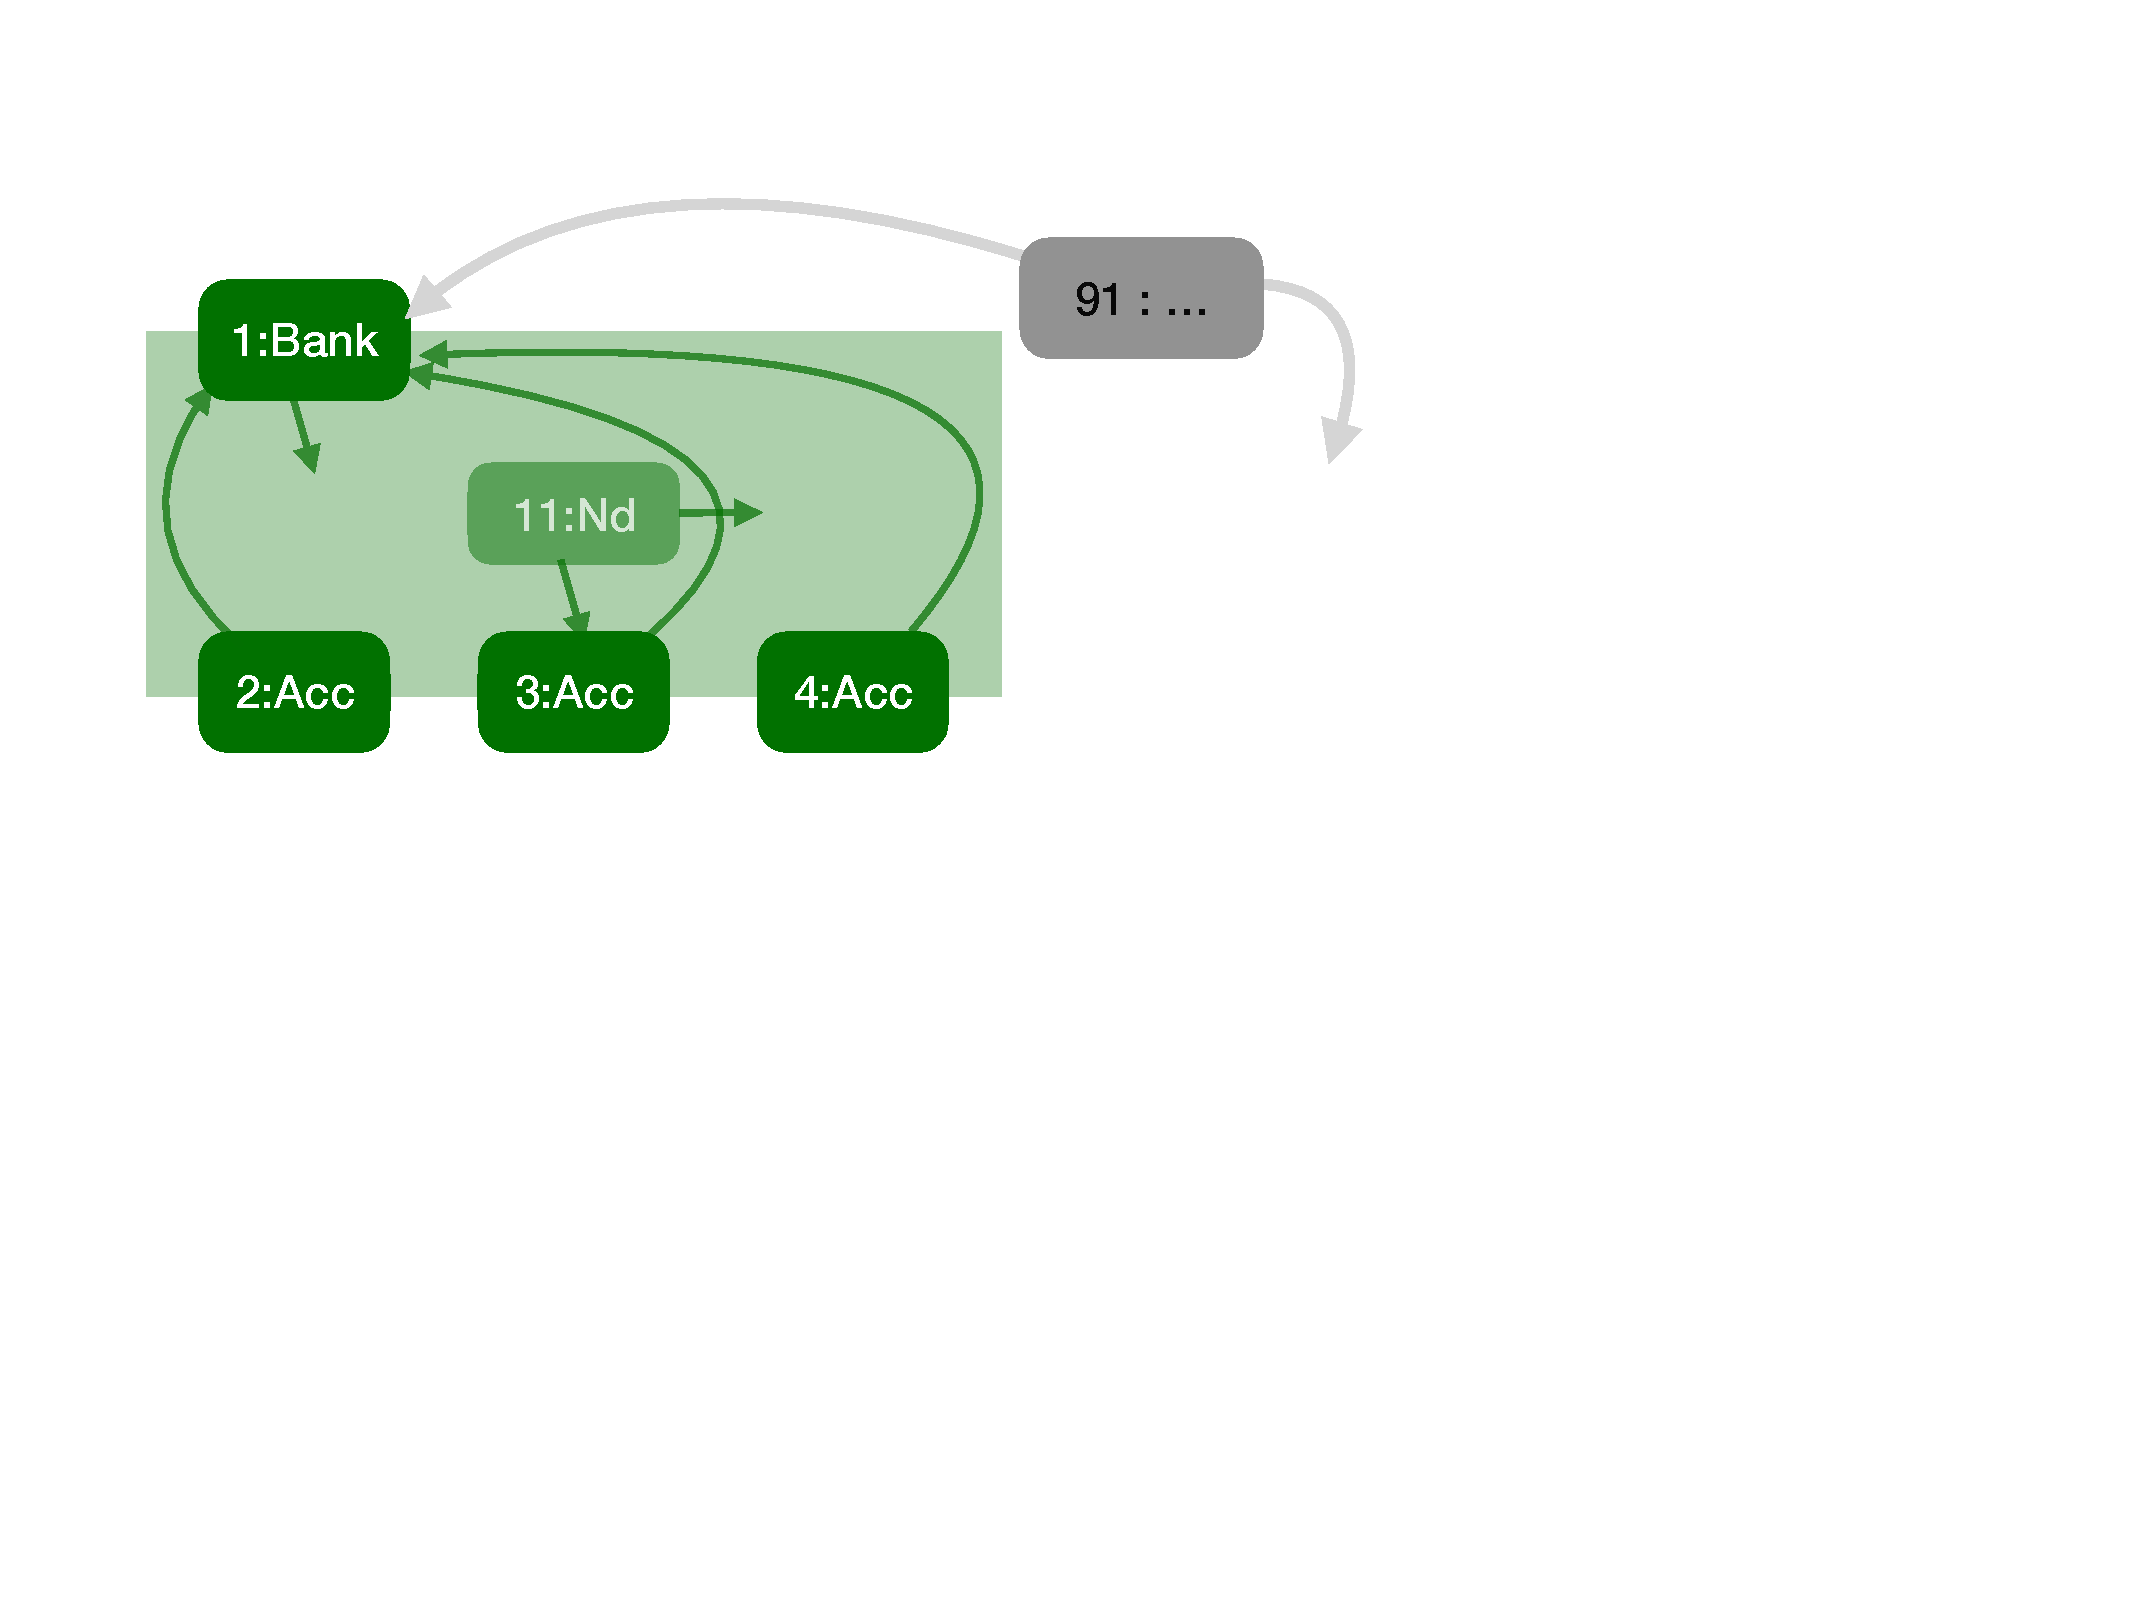
\includegraphics[width=\linewidth, trim=55  330 320 60,clip]{diagrams/BankAccount_version_2a.pdf}
   \end{minipage}
\end{tabular}
 
\sd{Note in the diagram above the dangling pointers at objects $1$,  $11$, and $91$ - reminiscent of the separation
of heaps into disjoint subheaps, as provided by the 
$*$ operator in separation logic \cite{Reynolds02}. The difference is that in separation logic, the 
separation is provided through the assertions, where $\A * \A'$ holds in any heap  which can be split into
disjoint $\chi$ and $\chi'$ where $\chi$ satisfies $\A$ and $\chi'$ satisfies $\A'$. That is, in $\A * \A'$  the split of the 
heap is determined by the assertions   $\A$ and $\A'$ and there is an implicit requirement of disjointness, while in $\restrct {\sigma}{\prg{S}}$ the split is
determined by \SF, and no disjointness is required.
}

We now define the semantics of $\Using {\A} {\prg{S}}$.


\begin{definition}[Space]  \label{def:valid:assertion:space} 
For any modules $\M$, $\M'$, assertions $\A$ and variable \prg{S}, we define$:$
\begin{itemize}
\item
 $\M\mkpair \M', \sigma \models \Using {\A} {\prg{S}}$
 \IFF
 $\M\mkpair \M', \restrct \sigma {\prg{S}} \models  \A  $.
\end{itemize}
\end{definition}
\jm{
\begin{definition}[Space]  \label{def:valid:assertion:space} 
For any modules $\M$, $\M'$, assertions $\A$ and variable \prg{S}, we define$:$
\begin{itemize}
\item
 $\M\mkpair \M', \sigma_0 \ldots \sigma \models \Using {\A} {\prg{S}}$
 \IFF
 $\M\mkpair \M', \sigma_0 \ldots \restrct \sigma {\prg{S}} \models  \A  $.
\end{itemize}
\end{definition}
 }

\sd{
The set \SF\ in the assertion $\Using {\A} {\prg{S}}$ is related to  framing  from implicit dynamic frames \cite{IDF}:
 in an implicit dynamic frames assertion  \ $\textbf{acc}\, \prg{x.f}  * \A$, the frame $\prg{x.f}$ prescribes which locations
 may be used to determine validity of $\A$.
The difference is that frames are sets of locations (pairs of address and field), while our \prg{S}-es are sets of addresses.
 More  importantly,   implicit dynamic frames assertions whose frames are not large enough are badly formed, 
 while in our work, such assertions
are allowed and may   hold %(\eg $\M_{BA2}\mkpair \M', \sigma  \models \Using {(\not(\exists n.\acc_2.\prg{balance}=n))} {\prg{S}_4}$),  
or not, \eg   %$\M_{BA2}\mkpair \M', \sigma   \models \exists n.\acc_2.\prg{balance}=n$, while 
 $\M_{BA2}\mkpair \M', \sigma_0 \ldots \sigma  \models \neg\ \Using {(\exists n.\acc_2.\prg{balance}=n)} {\prg{S}_4}$.
} 
 
 

\subsection{Satisfaction of Assertions - Time}
\label{sect:time} 
\sd{To deal with time, we are faced with four challenges: (a) the current configuration needs to store the code being executed, so
as to be able to calculate future configurations, (b) when considering the future, we do not want to observe 
configurations which go beyond the frame currently at the top of the stack, (c) there is no "undo" operator to deterministically enumerate
all the previous configurations.} 

\mrr[Through working with addresses instead of names, and instead requiring addresses to be bound to a name explicitly, we avoid the need to adapt the future configuration to use the current configuration's bindings. This would otherwise be necessary to allow the specification to keep the meaning of names consistent. Explicitly binding the name to an instance once renders it irrelevant if that binding changes over time, as the address will not, providing a time-independent handle to the same instance. It also allows for further flexibility over when the binding occurs, allowing for assertions referencing the past or future values of a certain binding.]{This read "validity of assertions in the future or the past needs to be judged in the 
future configuration, but using the bindings from the current one", however this is no longer the case. Consequently, the discussion of this challenge has been removed.\\
This has since been rewritten again to clear up the language; I am \textbf{unsure if the discussion over future/past bindings are helpful}, I'm doubtful right now because this seems kind of silly. }

\sd{
We address challenge (a) by storing the remaining code to be executed in \prg{cntn} in each frame. 
We address challenge (b) by \mrr[defining constrained reduction, where we only take]{Should there be more discussion of constrained reduction?} the top of the frame when considering future executions.
Finally, we address challenge (c) \mrr[by considering only configurations which arise from a given initial configuration, and 
which lead to the current configuration]{This originally said "from an initial configuration" without the "given". Does the introduction of explicit initial configurations have a further impact?}. 
}


\begin{definition}[Time Assertions]  \label{def:valid:assertion:time}
For any modules $\M$, $\M'$, and assertion  $\A$ we define

\begin{itemize}
% \item
% $\M\mkpair \M', \sigma \models   \Changes{\prg{e}}$  \IFF
% $\exists \sigma'.\, [\ \ \M\mkpair \M',\sigma \leadsto \sigma' \ \wedge \interp{e}{\sigma} \neq \interp{e}{\sigma\triangleleft \sigma'} \ \  ]$.
 \item
  $\M\mkpair \M', \sigma \models  \Next \A $
  \IFF
  $\exists \sigma'.\, [\ \ \M\mkpair \M',(\phi, \chi) \leadsto  \sigma' \ \wedge \M\mkpair \M',\sigma\adapt\sigma' \models \A \ \  ]$,
 \\
$\strut ~ \hspace{1.4in} $ \hfill  and where $\sigma$=$(\phi\cdot\_,\chi)$.\item
  $\M\mkpair \M', \sigma \models  \Future \A $
  \IFF
  $\exists \sigma'.\, [\ \ \M\mkpair \M',(\phi, \chi) \leadsto^* \sigma' \ \wedge \M\mkpair \M',\sigma\adapt\sigma' \models \A \ \  ]$,
 \\
$\strut ~ \hspace{1.4in} $   \hfill   and where $\sigma$=$(\phi\cdot\_,\chi)$.  
  \item
 $\M\mkpair \M', \sigma \models  \Prev \A $ \IFF
 $\forall \sigma_1, \sigma_2. [\ \ \Initial{\sigma_1}\ \wedge \   \M\mkpair \M', \sigma_1  \leadsto^*  \sigma_2 $\\
 $\strut ~ \hspace{2.1in}   \wedge \   \M\mkpair \M', \sigma_2  \leadsto   \sigma  
 \ \  \ \longrightarrow \ \ \   \
 \M\mkpair \M', \sigma\adapt\sigma_2  \models \A\ \
 ]$ 
 \item
 $\M\mkpair \M', \sigma \models  \Past \A $ \IFF
% $\forall \sigma_1, ... \sigma_n. [\ \ \Initial{\sigma_1}\ \wedge \  \sigma_n=\sigma $\\
% $\strut ~ \hspace{1.9in}   $   \hfill   $  \wedge \ \ \forall  i\in[1..n). \M\mkpair \M', \sigma_{i} \leadsto  \sigma_{i+1}$
% $\strut ~ \hspace{1.9in} $   \hfill   $ \longrightarrow \ \ \ ( \  \exists j\in [1..n-1).
% \M\mkpair \M', \sigma\adapt\sigma_j  \models \A\ \
%
$\forall \sigma_1. [\ \ \Initial{\sigma_1}\ \wedge \  \M\mkpair \M',\sigma_1 \leadsto^* \sigma \longrightarrow $\\
 $\strut ~ \hspace{0.1in} $   \hfill   $(\ \  \exists \sigma_2.
 \M\mkpair \M',\sigma_1 \leadsto^* \sigma_2 \ \wedge\  \M\mkpair \M',\sigma_2 \leadsto^* \sigma \ \wedge \ 
 \M\mkpair \M', \sigma\adapt\sigma_2  \models \A\ \ 
 )]$ 
\end{itemize}
\end{definition}
\mrr{Replaced $\phi\cdot\_$ with $\phi$ since there is no concept of \prg{nil : List a} here, single elements are counted as lists} 
\jm{
\begin{definition}[Constrained Reduction]  \label{def:constrained_reduction}
For any modules $\M$, $\M'$, and configurations $\sigma_1$, $\sigma_2$
\begin{itemize}
\item
$\M\mkpair \M',  \sigma_1\lceil\leadsto\rceil \sigma_2$ 
\IFF
$\M\mkpair \M',  (\phi, \chi_1) \leadsto(\psi, \chi_2)$\\
$\strut ~ \hspace{1.4in} $ \hfill 
where
$\sigma_1 = (\phi \cdot \psi_1, \chi_1)$ and $\sigma_2 = (\psi \cdot \psi_1, \chi_2)$
and
\item
$\M\mkpair \M',  \sigma_1\lceil\leadsto^*\rceil \sigma_2$ 
\IFF
$\M\mkpair \M',  (\phi, \chi_1) \leadsto^* (\psi, \chi_2)$\\
$\strut ~ \hspace{1.4in} $ \hfill 
where
$\sigma_1 = (\phi \cdot \psi_1, \chi_1)$ and $\sigma_2 = (\psi \cdot \psi_1, \chi_2)$
\end{itemize}
\end{definition}
\begin{definition}[Time Assertions]  \label{def:valid:assertion:time}
For any modules $\M$, $\M'$, and assertion  $\A$ we define
\begin{itemize}
% \item
% $\M\mkpair \M', \sigma \models   \Changes{\prg{e}}$  \IFF
% $\exists \sigma'.\, [\ \ \M\mkpair \M',\sigma \leadsto \sigma' \ \wedge \interp{e}{\sigma} \neq \interp{e}{\sigma\triangleleft \sigma'} \ \  ]$.
 \item
  $\M\mkpair \M', \sigma_0 \ldots \sigma \models  \Next \A $
  \IFF
  $\exists \sigma'.\, [\ \ \M\mkpair \M',\sigma \lceil\leadsto\rceil \sigma' \ \wedge \M\mkpair \M',\sigma_0 \ldots \sigma \models \A \ \  ]$
  \item
  $\M\mkpair \M', \sigma_0 \ldots \sigma \models  \Future \A $
  \IFF
  $\exists \sigma'.\, [\ \ \M\mkpair \M',\sigma \lceil\leadsto^*\rceil \sigma' \ \wedge \M\mkpair \M',\sigma_0 \ldots \sigma \models \A \ \  ]$
  \item
 $\M\mkpair \M', \sigma_0 \ldots \sigma \models  \Prev \A $ \IFF
$\forall \sigma'. [\ \  \M\mkpair \M',\sigma_0 \leadsto^* \sigma' \wedge \M\mkpair \M',\sigma' \leadsto \sigma \longrightarrow $\\
 $\strut ~ \hspace{0.1in} $   \hfill 
$ \M\mkpair \M', \sigma_0 \ldots \sigma'  \models \A\ \ 
 ]$ 
 \item
 $\M\mkpair \M',\sigma_0 \ldots  \sigma \models  \Past \A $ \IFF
$\forall \sigma'. [\ \  \M\mkpair \M',\sigma_0 \leadsto^* \sigma' \wedge \M\mkpair \M',\sigma' \leadsto^* \sigma \longrightarrow $\\
 $\strut ~ \hspace{0.1in} $   \hfill   
 $\M\mkpair \M', \sigma_0 \ldots \sigma'  \models \A\ \ 
 ]$ 
\end{itemize}
\end{definition}
}

%Thus,  $\M\mkpair \M', \sigma \models  \Future \A $ holds if
%$\A$ holds in some configuration $\sigma'$ which arises from execution of $\phi$, where $\phi$ is the top frame of $\sigma$. By requiring that $\phi \leadsto^* \sigma' $ rather than
%$\sigma \leadsto^* \sigma' $ we are restricting the set of possible future configurations to
%just those that are caused by the top frame;
%that is, we do not want to consider the effect of  enclosing function calls.
%
%This allows us to write more natural specifications
%when giving necessary conditions for some future effect.
 
 In general, $\Using {\Future {\A}} {\SF}$ is different from
  $\Future {\Using {\A} {\SF}}$. In the former assertion, $\SF$ must contain
   every extant object involved in reaching the future configuration, whilst in the latter, 
     $\SF$ needs instead to contain the objects needed to establish $\A$ in that future configuration.
    % chopped as the example no longer works.
  For example, revisit Fig. \ref{fig:BankAccountDiagrams}, and take $\SF_1$ to consist of objects \prg{1}, \prg{2},   \prg{4}, \prg{93}, and \prg{94},
  and $\SF_2$ to consist of objects \prg{1}, \prg{2},   \prg{4}.  Assume that 
   $\sigma_5$ is like $\sigma_1$, that the next call in $\sigma_5$ is a method on $\prg{u}_{94}$, whose  body obtains the
  address of $\acc_4$ (by making a call on \prg{93} to which it has access), and the address of $\acc_2$ (to which it has access),
  and then makes the call $\acc_2.\prg{deposit}(\acc_4,360)$. Assume also     that $\prg{a}_4$'s balance is \prg{380}.
  %Assume   that $\sigma_1$ contains the
  % call $\prg{m()}$ with receiver $\pu_{94}$ and that the code of \prg{m} and \prg{m2} is as above. 
  Then\\
  $\strut$ \hspace{1.1cm}  $\M_{BA1}\mkpair ..., \sigma_0 \ldots \sigma_5 \ \models \ \Using {\Future{ \Changes {\acc_2.\bal}}} {\SF_1}$\\
   $\strut$ \hspace{1.1cm}  $\M_{BA1}\mkpair ..., \sigma_0 \ldots \sigma_5 \ \not\models \ \Using {\Future{ \Changes {\acc_2.\bal}}} {\SF_2}$\\
 $\strut$ \hspace{1.1cm}  $\M_{BA1}\mkpair ..., \sigma_0 \ldots \sigma_5 \ \models \ \Future{ \Using {\Changes {\acc_2.\bal}} {\SF_2}}$\

Whilst the above shows that from $\Future { \Using{A}{\SF} }$ we cannot conclude $\Using { \Future{A} }{\SF}$, it is also worth noting that in general the inverse doesn't hold either. $\Future { \Using{A}{\SF} }$ restricts $A$ in the future, meaning any objects instantiated in the between the present and then are excluded, whereas $\Using { \Future{A} }{\SF}$ restricts the space in the present, so the objects are considered in A. Taking a new configuration $\sigma_6$  with continuation \prg{x := new Account(100, null) } and otherwise similar to $\sigma_1$, and $\SF = \emptyset$, we cannot prove $\M_{BA1}\mkpair ..., \sigma_0 \ldots \sigma_6 \ \models \ \Future{ \Using { \prg{x.bank} = \prg{null} } {\SF}}$  as \prg{x} is not in $S$, however, we can prove $\M_{BA1}\mkpair ..., \sigma_0 \ldots \sigma_6 \ \models \ \Using { \Future{ \prg{x.bank} = \prg{null} } } {\SF}$, since the restriction of the configuration to $\SF$ in the present doesn't prevent the next statement's new \prg{Account} being considered in the \Future{\cdot}.


\subsection{Properties of Assertions}

 
\label{sect:classical} 
We define equivalence of   assertions in the usual way: assertions $\A$ and $\A'$are equivalent if they are satisfied  in
the context of the same configurations and module pairs -- \ie\\
 \strut\mrr{Is adding $\sigma_0$ okay like this?} \hspace{1.1cm} $\A \equiv \A'\  \IFF\    \forall \sigma_0, \sigma.\, \forall \M, \M'. \ [\ \ \M\mkpair \M', \sigma_0\ldots\sigma \models \A\ \mbox{ if and only if }\ \M\mkpair \M', \sigma_0\ldots\sigma \models \A'\ \ ].$\\
We can then prove that the usual equivalences hold, \eg\  $ \A \vee \A' \ \equiv \  \A' \vee \A$, and\   $\neg (\exists \prg{x}.\A )  \  \ \equiv \  \forall \prg{x}.(\neg  \A)$.
%
Our assertions are classical, \eg  $ \A \wedge\neg \A \ \equiv \  \prg{false}$, and $\M\mkpair \M', \sigma_0 \ldots \sigma  \models \A$ and  $\M\mkpair \M', \sigma_0 \ldots \sigma  \models \A \rightarrow \A'$  implies
$\M\mkpair \M', \sigma_0 \ldots \sigma  \models \A '$. 
 \sd{This desirable property comes at the loss of some expected equivalences, \eg, in general, 
 $\e = \prg{false}$ and $\neg\e$ are not equivalent. 
 More  in Appendix \ref{app:assertions}.}

\subsection{Modules satisfying assertions}

Finally, we define satisfaction of assertions by modules: a module
$\M$ satisfies an assertion $\A$ if for all other potential modules $\M'$, in all configurations arising from executions of $\M\mkpair\M'$, the assertion $\A$ holds.

\begin{definition}
\label{def:module_satisfies}
For any module $\M$, and  assertion $\A$, we define:
\begin{itemize}
\item
$\M \models \A$ \IFF  $\forall \M'.\, \forall \ \sigma\!\in\!\Arising{\M\mkpair\M'}.\   \M\mkpair\M', \sigma \models \A$
\end{itemize}
\end{definition}

\jm{
\begin{definition}
\label{def:module_satisfies}
For any module $\M$, and  assertion $\A$, we define:
\begin{itemize}
\item
$\M \models \A$ \IFF  $\forall \M'.\, \forall \sigma_0, \Initial{\sigma_0}, \ \sigma\!\in\!\Arising{\M\mkpair\M', \sigma_0}.\   \M\mkpair\M', \sigma_0 \ldots \sigma \models \A$
\end{itemize}
\end{definition}
}

 






\section{Another Example -- Attenuating the DOM}
%\sdcomment
\sophia{This section now needs to be updated, as it has moved to later in the paper}
\label{sect:example:DOM}
%We will now discuss  an example demonstrating the need to describe attenuation in specifications.
In this section we look at a couple of examples from the literature where a holistic specification would provide obvious benefits in ensuring robustness.
\subsection{Attenuating the DOM}
\label{sect:example:DOM}

\emph{Attenuation} is the ability to provide an untrusted client \emph{restricted}  access to an object's functionality. This is usually achieved through the introduction of an intermediate object. Such intermediate objects --- protection proxies \cite{gof} --- are a common design pattern, and their security properties have been studied at length in the object capabilities literature \cite{MillerPhD,murray10-infoflow}.

\citet{dd} proposed specifications for attenuation of trees of DOM  nodes.
Access to a DOM node
gives access to its parent and all its children nodes, and the ability to
modify the properties of any accessible node. As the top nodes of the
tree usually contain privileged information (such as web content
showing your banking details) while the lower nodes contain less
crucial information (such as advertisements for BREXIT) we want to be
able to limit access given to third parties to only the lower part of
the DOM tree (so that Jacob Rees-Mogg cannot access your bank
account). We do this through a \prg{Wrapper}, which has
a field \prg{node} pointing to a \prg{Node} in the underlying DOM, and a field \prg{height}.
\forget{
which restricts the range of \prg{Node}s which may be modified through
the use of the particular \prg{Wrapper}.Namely, }
When you hold
a \prg{Wrapper} you can modify the \prg{property} of all the
descendants of the \prg{height}-th ancestors of the \prg{node} of that
particular \prg{Wrapper}. 
\forget{ It is not difficult to write such
a \prg{Wrapper}; a possible implementation appears in
Figure \ref{fig:DOM} in appendix \ref{DOM:traditional}.}


Figure \ref{fig:WrapperUse} shows a
\prg{Wrapper} object attenuating the use of 
\prg{Node}s.
The
function \prg{usingWrappers} has as its parameter an object of unknown
provenance, here called \prg{unknwn}. We create a tree
consisting of nodes \prg{n1}, \prg{n2}, ... \prg{n6}, depicted as blue
circles on the right-hand-side of the Figure and a
wrapper for \prg{n5} with height \prg{1}. This means that the
wrapper \prg{w} may be used to modify
 the objects in the green triangle, while it cannot be used to
modify the objects within the
blue triangle.  We call a function named \prg{untrusted} on
the \prg{unknwn} object, and pass \prg{w} as argument.

\begin{figure}[htb]
\begin{tabular}{llll}
\ \ &
\begin{minipage}{0.45\textwidth}
\begin{lstlisting}
func usingWrappers(unknwn){
   n1=Node(null,"fixed"); 
   n2=Node(n1,"robust"); 
   n3=Node(n2,"volatile"); 
   n4=Node(n2,"const");
   n5=Node(n3,"variable");
   n6=Node(n3,"ethereal");
   w=Wrapper(n5,1);
   
   unknwn.untrusted(w);
   
   assert n2.property=="robust" 
   ...
}
\end{lstlisting}
\end{minipage}
& & 
\begin{minipage}{0.75\textwidth}
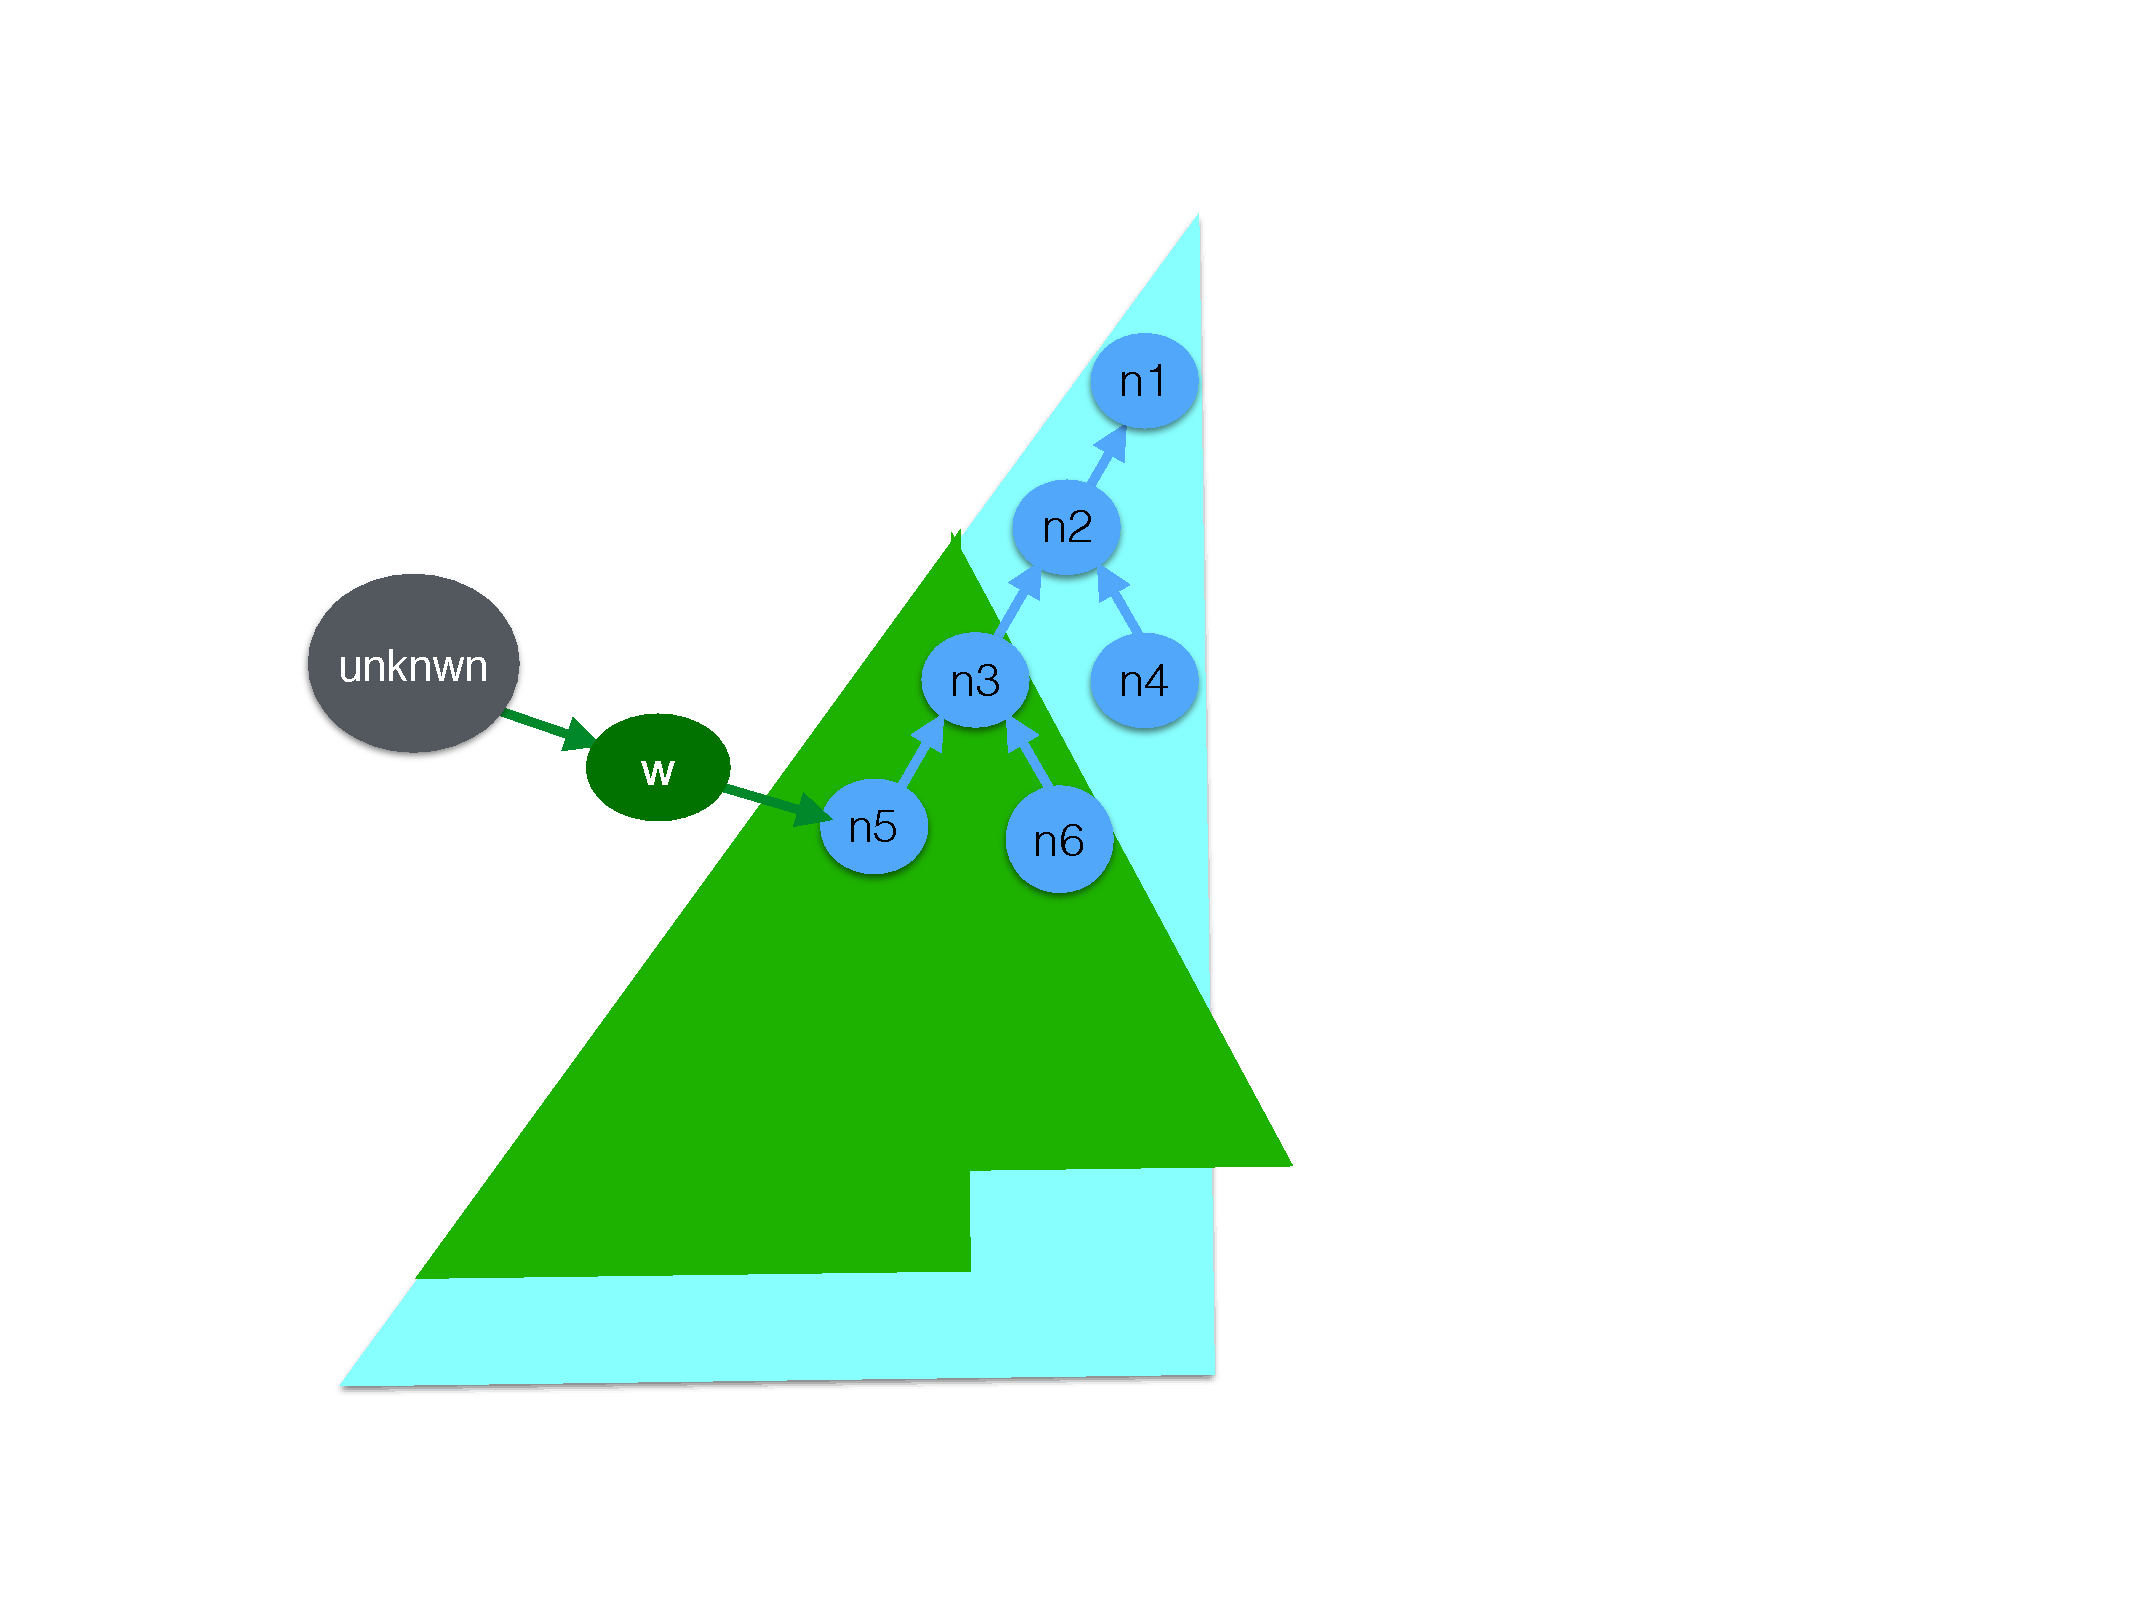
\includegraphics[width=\linewidth, trim=145  320 60 105,clip]{diagrams/DOM.pdf}
% x y z w
% y seems to eat up the bollom
% y=320 is good
% x eats space from left, if you increase it the diagram decreases from left
% w eats space from top, if you increase it the diagram decreases from top
% w=100 is good
%\includegraphics[page=3, width=\linewidth, trim=150  270 40 150, clip]{diagrams/snmalloc.pdf}
%\sdcomment{I think we need to change the diagram so that it says small slab.}
\strut \\
\strut \\

\end{minipage}
\end{tabular}
 \vspace*{-4.5mm}
\caption{\prg{Wrapper}s protecting \prg{Node}s }
\label{fig:WrapperUse}
\end{figure}

Even though we know nothing about the \prg{unknwn} object or
its \prg{untrusted} function, and even though the call gives
to \prg{unknwn} access to \prg{w}, which in turn has transitively
access to the entire tree, we know that %the call to
the \prg{untrusted} function will not
affect the \prg{property} fields of the nodes \prg{n1}, \prg{n2},
and \prg{n4}.  Thus, the assertion is guaranteed to
succeed.  The question is how do we specify \prg{Wrapper}, so as to be
able to make such an argument. %prove this assertion.

A specification of the class \prg{Wrapper} in the traditional
style, \cite{Leavens-etal07} \forget{\cf appendix \ref{DOM:traditional})}
consists of pairs of PRE- and POST- conditions for each of the
functions of that class. 
\forget{Each such pair gives a {\em sufficient}
condition for some effect to take place: for example the
call \prg{w.setProperty(i,prp)} where \prg{i} is smaller
than \prg{w.height} is a sufficient condition to modify \prg{property}
of the \prg{i}-th parent of \prg{w.node}. But we do not know what
other ways there may be to modify a node's \prg{property}.}  
A broken
wrapper could accidentally permit access to nodes one or two levels
above the expected height due to off-by one errors. More seriously,
a malicious wrapper could offer a
back-door public accessor method that leaks the underlying DOM
object through the wrapper, returning direct access to any of the
other nodes in the DOM, or even to queue a task to
delete every property at midnight GMT on 29 March 2019. All of these errors are possible while
preserving the PRE- and POST- conditions expected of a \prg{Wrapper}. 

\forget{
What is needed here is some way to specify the \emph{necessary
conditions}
under which some change could be made: if some external client is to
change a node's property, then  that client must have either direct
access to a node in that DOM tree, or indirect access via a wrapper
configured so that it can change the affected node.
Thus,
% \sdcomment
\sophia{Shall we say the following, or does it break the flow?  
"Moreover, on line 10 we do not know which functions are called
on \prg{w}."
\kjx{I put that in and expanded on it. We need to explain the issues I think}
I do not see where it is}

% I think the below should be clear by niw
% In this work, we propose \emph{holistic specifications}, which
%describe the behaviour of an abstract data type as a whole, taking all
%possible method calls into account. Such holistic specifications
%emphasize the \emph{necessary conditions} for some effect to take
%place over the sufficient conditions as in traditional
%specifications. In our example:
}
%
%%KJX things there needs to be someting linking this quote to the
%%previous para...
%
An holistic specification can prevent these problems:
%
\begin{quote}
The \emph{necessary} condition for the modification of \prg{nd.property} for some \prg{nd} of class \prg{Node}  is either access to some   \prg{Node} in the same tree, or  access to a \prg{w} of class \prg{Wrapper} where the \prg{w.height}-th parent of \prg{w} is an ancestor of \prg{nd}.
\end{quote}

\noindent Or in \Chainmail:

%
% Having justified the need for  necessary conditions in specifications, 
%
%To give a flavour of \Chainmail, we use it  express the requirement from above:
%  This  gives us the opportunity to  demonstrate primitives for time ($\Future{\_}$) and authority ($\Changes{\_}$ and $\Using {\_} {\_}$).
 % and   more traditional relations between objects ( $\prg{nd}.\prg{parnt}^k\!=\! ...$):
% $\strut$ 
\vspace{.1cm}

\noindent
% \begin{quote}
$\forall \prg{S}:\prg{Set}.\forall \prg{nd}:\prg{Node}.$\\
$[\ \ {\Using{\Future {\Changes {\prg{nd.property}}}}  {\prg{S}}}$ \\
$\strut  \ \ \longrightarrow$\\
$\strut \ \ \ \exists \prg{o}:\prg{Object}[\ \prg{o}\in\prg{S}\ \ \wedge\ \ \neg(\prg{o}:\prg{Node})\ \ \wedge\  \ \neg(\prg{o}:\prg{Wrapper})\ \ \ \wedge \  $\\
$ \strut\ \ \  \ \ \ \ \ \ \ \ [\ \exists \prg{nd}':\prg{Node}. \CanAccess{\prg{o}}{\prg{nd}'}\  \ \ \  \vee$\\
$ \strut\ \  \ \  \ \  \ \ \ \ \ \ \ \exists \prg{w}:\prg{Wrapper}.\exists k\!:\!\mathbb{N}.
% $\\ $ \strut \ \ \ \ \ \ \ \ \ \ \ \ \ \ \ \ \  \ \ \
  (\ \CanAccess{\prg{o}}{\prg{w}}  \ \wedge\ \prg{nd}.\prg{parnt}^k\!=\!\prg{w.node}.\prg{parnt}^{\prg{w.height}}) \ \ \ ]\ ]$\\
$ ]$
% \end{quote}

\vspace{.1cm}
\noindent
That is, if the value of \prg{nd.property} is modified
($\Changes{\_}$) at some future time ($\Future{\_}$) and if reaching
that future time involves no more objects than those from set \prg{S}
(\ie ${\Using{\_} {\prg{S}}}$), then at least one (\prg{o}) of the
objects in \prg{S} is not a \prg{Node} nor a \prg{Wrapper},
and \prg{o} has direct access to some node
($\CanAccess{\prg{o}}{\prg{nd}'}$), or to some wrapper \prg{w} and
the \prg{w.height}-th parent of \prg{w} is an ancestor of \prg{nd}
(that is,
$\prg{parnt}^k\!=\!\prg{w.node}.\prg{parnt}^{\prg{w.height}}$).
%
% It is important to clarify what we mean by ``access''. 
%
With this specification, we can ensure
% prove that the assertion will succeed ensuring
that all future updates of
the \prg{Wrapper} class will continue to
% meet that specification, guaranteeing the protection of
protect the DOM.
%\prg{Node} data. 


\forget{
Definitions of these concepts appear later
(Definition \ref{def:valid:assertion}), but note that our ``access''
is intransitive: $\CanAccess x y$ holds if either \prg{x} has a field
pointing to \prg{y}, or \prg{x} is the receiver and \prg{y} is one of
the arguments in the executing method call.
 
In the next sections we proceed with a formal model of our model. In the appendix we discuss more -- and simpler -- examples.
We chose the DOM for the introduction, in order to give a flavour of the \Chainmail features.
}
 



\section{Discussion}
\label{sec:discussion} 

\paragraph{Specification Language}

\kjx{this section is new, but James didn't really know what Sophia wanted.}

The key to writing and using holistic specifications is to capture the
implicit assumptions underlying the design of the system we are
specifying.  The design principle animating the design of \Chainmail\
is to make writing holistic specifications as straightforward as
possible.

This is why we support bi-directional temporal operators (``will'',
``was'' etc) rather than just one temporal direction. Some assertions
are easier to express looking forwards (if a vending machine takes a
coin it will eventually dispense a chocolate bar) while other
assertions as easier to express looking backwards (if a vending
machine dispenses a chocolate bar, it has already accepted the coin
to pay for it).

Similarly, in an imperative setting, the question of whether a change can
occur at all is at least as important as the precise details of the
change. This is why we support the ``changes'' operator in \Chainmail;
to enable specifications to capture that notion directly, rather than
e.g.\ expressing explicit differences in values between pre- and post-
states.

For modelling the open world, the interactions between the external
and internal modules are essential.   \kjx{doesn't know what more to
say here someone else can fill it in} 
We included predicates in \Chainmail to be able to state explicitly which side of the boundary between modules an object is and what can cross that boundary.

The issues we have had to deal with are those related to space in
various ways: ``access'', ``in'', and ``external''.  One object
referring to another appears simple enough on the surface, but causes
significant problems in an open world setting. In \Chainmail, these
problems appear with universal quantification on the source of a
reference: ``in'' enables us to bound these quantifications.



\paragraph{Underlying Language}

\kjx{pulled in from earlier version}

For our underlying language, we have chosen an object-oriented, class based language,
\sd{but we  expect that the ideas} will also be
applicable to other kinds of languages (object-oriented or
otherwise).
%% \sd{We  could, \eg} extend our work to prototype-based programming
%% by creating an (anonymous) class to reify each
%% prototype \cite{graceClasses}. 
%
We have chosen to use a dynamically typed language because many of the
problems we hope to address are written in these
languages: web apps and mashups in Javascript; backends in Ruby or
PHP.  We expect that supporting types would make the problem easier,
not harder, but at the cost of significantly increasing the complexity
of the trusted computing base that we assume will run our programs. In
an open world, without some level of assurance (e.g. proof-carrying
code) about the trustworthiness of type information: unfounded
assumptions about types can give rise to new vulnerabilities that
attackers can exploit \cite{pickles}.

Finally, we don't address inheritance. As a specification language,
individual \Chainmail assertions can be combined or reused without any
inheritance mechanism: the semantics are simply that all
the \Chainmail\ assertions are expected to hold at all the points of
execution that they constrain.  \LangOO\ does not contain inheritance
simply because it is not necessary to demonstrate specifications of
robustness: whether an \LangOO class is defined in one place, or
whether it is split into many multiply-inherited superclasses, traits,
default methods in interfaces or protocols, etc.\ is irrelevant,
provided we can model the resulting (flattened) behaviour of such a
composition as a single logical \LangOO\ class.

% Julian: below is some discussion about the coq proofs.
\begin{itemize}
\item
\begin{enumerate}
\item
Lemma 5 (Assertions are Classical-1)
\item
Lemma 6 (Assertions are Classical-2)
\end{enumerate}
\end{itemize}


% SD removed, as some of this is in Related work
%\paragraph{Contracts and Preconditions}
%
%Traditional specification languages based on pre- and post-conditions
%are generally based on design-by-contract assumptions: ``if the
%precondition is not satisfied, the routine is not bound to do
%anything'' \cite{meyer92dbc} --- that is, the routine can do
%anything. Ensuring preconditions is the responsibility of the caller,
%and if the caller fails to meet that responsibility it is not the
%responsibility of the invoked function to fix the problem \cite{Mey88}.
%Underlying this approach, however, is the assumption of a closed
%system: that all the modules in a system are equally trusted, and so
%inserting redundant tests would just make the system more complex and
%more buggy. Indeed, \citet{meyer92dbc} states that ``This principle is
%the exact opposite of the idea of defensive programming.''
%
%In an open world, however, we do not have the luxury of trusting the
%other components with which we interact --- indeed we barely have the
%luxury of trusting ourselves.  We must assume that our methods may be
%invoked at any time, with any combination of arguments the underlying
%platform will support, irrespective of the overall state of the
%system, or of the object that receives the method request: in some
%sense, this is the very definition of an open system in an open world.
%Since methods cannot control when they are invoked, we must work
%as if all (potentially) externally-visible methods just have the precondition
%\prg{true} --- and we had better be very careful about any assumptions
%we make about which method or objects are in fact externally visible
%and which are not.  
%%\susan{I like it too.}\kjx{likes this sentence: 
%\sd{Holistic specifications directly support robust programming by making those kinds of
%assumptions explicit, giving the necessary conditions under which
%effects may take place and objects may become accessible, and then can
%help programmers ensure their programs maintain those conditions.}
%% WAS, but SD argues it is not right
%%Holistic specifications
%%directly support robust programming by making those kinds of
%%assumptions explicit, giving the necessary conditions under which
%%objects should be accessed or their methods invoked, and then can
%%help programmers ensure their programs maintain those conditions.}

 

%%% it's a point James would like made somewhre? but where?



%% \paragraph{Necessary v.s.\ sufficient conditions.}

%% Are the necessary conditions the same as the complement of all the
%% sufficient conditions?  The \sd{possible state transitions of a component are
%% described by the transitive closure of the individual transitions.
%% % , and
%% %the reachable states are those that are reachable from initial states through
%% %this transitive closure relation.
%% Taking  Figure \ref{fig:NecessaryAndSuff} part (a), if we calculate the 
%% complement of the transitive closure 
%% of the transitions, then we could, presumably, obtain all transitions which will not happen, 
%% and if we apply this relation to the set of initial states, we obtain all 
%% states guaranteed not to be reached.
%% Thus, using the sufficient conditions, we  obtain implicitly   
%% more fine-grained information than that  available through the yellow transitions and 
%% yellow boxes in Figure \ref{fig:NecessaryAndSuff}  part (b).}

%% \sd{This implicit approach} is mathematically sound. But it is impractical, brittle with
%% regards to software maintenance, and weak with regards to reasoning in
%% the open world.


%% \sd{The implicit approach} is impractical: it suggests that when interested in
%% a necessity guarantee a programmer would need to read the
%% specifications of all the functions in that module, \sd{and think 
%% about all possible sequences of such functions and all interleavings with 
%% other modules. }
%% What if the bank did indeed enforce that only the account owner may withdraw
%% funds, but had another function which allowed the manager to appoint
%% an account supervisor, and another which allowed the account
%% supervisor to assign owners?

%% \sd{The implicit approach} is also brittle with regards to software maintenance:
%%  it gives no guidance to the team maintaining a piece of
%% software.  If the necessary conditions are only implicit in the
%% sufficient conditions, then developers' intentions about those
%% conditions are not represented anywhere: there can be no distinction
%% between a condition that is accidental (if \sd{\prg{notify}-ing} is not
%% implemented, then it cannot be permitted) and one that is essential
%% (money can only be transferred by account owners).
%% Subsequent developers may inadvertently add functions which break these
%% intentions, without even knowing they've done so.

%% Finally, the implicit approach  is   weak when it comes to reasoning
%% about programs in an open world:  it does not give any
%% guarantees about objects when they are passed as arguments to calls
%% into unknown code. For example, what guarantees can we make about the
%% top of the DOM tree when we pass a wrapper pointing to lower parts of
%% the tree to an unknown advertiser?




%% \section*{Bibliography}
%%  \bibliographystyle{plain}
%%  \bibliography{Case}

%\section{Attic}
%Here is stuff that we deleted, but might like to reuse.

The following came from beginning of foundations:
\kjx{\textbf{all these points should (already) be made by the example - the
  first one probably as early as the intro}
 As we already stated, this work is devoted to the specification of code in the open world. For these we propose what we call {\em holistic specifications.}
%
We claim that the most pertinent aspects of behaviour in the open world
are   in terms of  {\em necessary} conditions (\eg what can cause -- what are necessary conditions for --
 the balance of an account to decrease), rather than sufficient conditions (\eg the owner of an account may
 call the \prg{transfer} function, and as a result the balance decreases).
Such necessary conditions are not attached to particular function calls or program points; they apply
throughout program execution.
Therefore, they are expressed through  {\em invariants} that can be observed throughout the lifetime of a program, rather than at specific points in program execution.
  }

\section*{APPENDIX -- examples}
\sdcomment{Note that the file rest.tex contains more material.}

 

\appendix

\section{The language \LangOO}
\label{sect:LangOO}
%\section{The language \LangOO}
%\label{sect:LangOO}
\subsection{Modules and Classes}
\label{secONE}

\LangOO programs consist of modules, which are repositories of code. Since we study class based oo languages,
in this work, code is represented as classes, and  modules are mappings from  identifiers to class  descriptions.

\begin{definition}[Modules]
\label{defONE}
We define $\syntax{Module}$ as  the set of mappings from identifiers to class descriptions (the latter defined in Definition \ref{def:syntax:classes}):\\  % to force line break

\begin{tabular}  {@{}l@{\,}c@{\,}ll}
\syntax{Module} \ \  &  \   $\triangleq $  \ &
   $ \{ \ \ \M \ \ \mid \ \  \M: \ \prg{Identifier} \   \longrightarrow \
  \  \syntax{ClassDescr}     \  \    \}$
 \end{tabular}
\end{definition}
 
Classes, as defined   below,
consist of field, method definitions and ghost field declarations.
 \LangOO is untyped, and therefore fields are declared without types, 
 method signatures and ghost field signatures consist of  sequences of parameters without types, and no return type.
 Method bodies consist of sequences of statements;
these can be field read or field assignments, object creation, method calls, and return statements.
All else, \eg booleans, conditionals, loops,  can be encoded.
Field read or write is only allowed \sd{if the object whose field is being read 
belongs to the same class as the current method. This is enforced by the operational semantics, \cf
Fig.  \ref{fig:Execution}.}
\sd{Ghost fields  are defined as implicit, side-effect-free functions with zero or more parameters. They are ghost information, \ie 
they are not directly stored in the objects, and are not read/written during execution. When such a ghostfield is
mentioned in an assertion, the corresponding function is evaluated. More in section \ref{sect:expressions}.
Observe that the expressions that make up the bodies of ghostfield declarations (\prg{e}) are more complex than the terms that 
appear in individual statements.}

From now on we expect that the set of field and the set of ghostfields defined in a class are disjoint.  

\label{sec:syntax:classes}


\begin{definition}[Classes]
\label{def:syntax:classes}
Class descriptions consist of field declarations, method declarations, ghostfield declarations, and, optionally, a constructor.
 
\begin{tabular}{lcll}
 \syntax{ClassDescr}   &   \BBC  &     \kwN{class}  \syntax{ClassId} \lp \x$^*$\rp    \lb\,  $($ \syntax{FieldDecl} $)^*$ $($ CDecl\ $)?$ \
 $($  \syntax{MethDecl}\ $)^*$   \   $($   \syntax{GhosDecl}\ $)^*$ \ \ \rb
\\
\syntax{FieldDecl} &\BBC& \kwN{field} \f \\
\syntax{CDecl} &\BBC&
     \kwN{constructor}\    \lp \x$^*$\rp     \lb\, \syntax{Stmts}  \,
    \rb
 \\
\syntax{MethDecl} &\BBC&
     \kwN{method}\    \m\lp \x$^*$\rp     \lb\, \syntax{Stmts}  \,
    \rb
 \\
 \syntax{Stmts}  &\BBC&  \syntax{Stmt}     ~\SOR~  \syntax{Stmt} \semi \syntax{Stmts} \\
\syntax{Stmt}    &\BBC&
      \x.\f {\kw{:=}} \x   ~\SOR~  \x{\kw{:=}}  \x.\f    ~\SOR~        \x  {\kw{:=}} \x.\m\lp \x$^*$\rp     ~\SOR~     \x  {\kw{:=}}     \newKW\, \c\,\lp \x$^*$\rp   ~\SOR~
   \returnKW \,  \x   \\
  \syntax{GhostDecl} &\BBC&  \kwN{ghost} \f\lp \ \x$^*$\ \rp \lb \  \SE\ \rb\\
 \SE  &\BBC&    \kwN{true}   ~\SOR~  \kwN{false}   ~\SOR~  \kwN{null}  ~\SOR~  \x  \   ~\SOR~  
     \   \SE=\SE    ~\SOR~ \kwN{if}\, \SE\,   \kwN{then}\,  \SE\,    \kwN{else}\, \SE    ~\SOR~  \SE.\f\lp\ \SE$^*$ \ \rp\\
 \x, \f, \m &\BBC&  \prg{Identifier} 
 \end{tabular}

  \vspace{.03in}
  \noindent
 where we use metavariables as follows:
 $\x \in  \syntax{VarId} \ \ \  \f \in  \syntax{FldId} \ \ \  \m \in  \syntax{MethId} \ \ \  \c \in  \syntax{ClassId}$, and  \x\ includes \this
\end{definition}


We define a method lookup function $\mathcal{M}$, which returns the corresponding method definition given a class \c\ and a method identifier \m, and similarly a ghostfield lookup function $\mathcal{G}$, and a constructor lookup function $\mathcal{C}$, which returns a default, field-filling constructor if one wasn't defined.

 \begin{definition}[Lookup] For a class identifier \prg{C}  and a method identifier \prg{m}$:$  $ ~ $ \\
\label{def:lookup}
\noindent
$
\Meths {} {\prg{C}} {m}       \triangleq  \ \left\{
\begin{array}{l}
                        \m\, \lp \p_1, ... \p_n \rp \lb Stmts\, \rb\\
\hspace{0.5in} \mbox{if}\  \M(\prg{C}) =   \kwN{class}\, \prg{C}\, \  \lb ...\,   \kwN{method}\, \m\, \lp \p_1, ... \p_n \rp \lb Stmts\,  \rb  ... \ \rb.
\\
\mbox{undefined},  \ \ \ \mbox{otherwise.}
\end{array}
                    \right.$
\\
$
{\mathcal G} (\M, {\prg{C}}, {\f})    \ \   \triangleq  \ \left\{
\begin{array}{l}
                        \f\, \lp \p_1, ... \p_n \rp \lb \prg{e}\  \rb\\
\hspace{0.5in} \mbox{if}\  \M(\prg{C}) =   \kwN{class}\, \prg{C}\, \  \lb ...\,   \kwN{ghost}\,  \m\, \lp \p_1, ... \p_n \rp \lb \prg{e} \  \rb  ... \ \rb.
\\
\mbox{undefined},  \ \ \ \mbox{otherwise.}
\end{array}
                    \right.$
\\
$
{\mathcal C} (\M, {\prg{C}})   \quad \ \,   \triangleq  \ \left\{
\begin{array}{l}
                        \kwN{constructor} \, \lp \p_1, ... \p_n \rp \lb Stmts\, \rb\\
\hspace{0.5in} \mbox{if}\  \M(\prg{C}) =   \kwN{class}\, \prg{C}\, \  \lb ... \, \kwN{constructor} \, \lp \p_1, ... \p_n \rp \lb Stmts\, \rb ... \ \rb.
\\
\kwN{constructor} \, \lp \p_1, ... \p_n \rp \lb \prg{this}.\f_1 \kw{:=} \p_1; ... \prg{this}.\f_n \kw{:=} \p_n\ \rb\\
\hspace{0.5in} \mbox{where}\  \M(\prg{C}) =   \kwN{class}\, \prg{C}\, \  \lb \kwN{field}\, \f_1\, ... \kwN{field}\, \f_n\ ... \ \rb.
\\
\mbox{undefined},  \ \ \ \mbox{otherwise.}
\end{array}
                    \right.$
  \end{definition}

\subsection{The Operational Semantics of \LangOO}
\label{formal:semantics}

We will now define execution of \LangOO code.
We start by  defining the  runtime entities, and runtime configurations, $\sigma$, which consist of heaps and stacks of frames.
 The frames are pairs consisting of a continuation, and a mapping from identifiers to values.
The continuation represents the code to be executed next, and the mapping gives meaning
to the formal and local parameters.

\begin{definition}[Runtime Entities]
\label{def:runtimeentities}
We define addresses, values, frames, stacks, heaps and runtime configurations.

\begin{itemize}
\item
We take addresses to be an  enumerable set,  \prg{Addr}, and use the identifier $\alpha\in \prg{Addr}$ to indicate an address.
\item
Values, $v$, are either addresses, or sets of addresses or null:\\
 $~ ~ ~ \ v \in \{ \prg{null} \} \cup \prg{Addr}\cup {\mathcal P}( \prg{Addr})$.
\item
  Continuations are either   statements  (as defined in Definition~\ref{def:syntax:classes}) or a marker, \x {\kw{:=}} $\bullet$, for a nested call followed by
  statements to be executed
  once the call returns.


\begin{tabular}{lcll}
\syntax{Continuation} &\BBC&   \syntax{Stmts} ~\SOR~   \x {\kw{:=}} $\bullet$ \semi\ \syntax{Stmts} \\
 \end{tabular}

\item
Frames, $\phi$, consist of a code stub  and a  mapping from identifiers to values:\\  $~ ~ ~ \ \phi \ \in\ \syntax{CodeStub} \times \prg{Ident} \rightarrow Value$,
\item
Stacks,  $\psi$, are sequences of frames, $\psi\ ::=   \phi \ | \ \phi\cdot\psi$.
\item
Objects consist of a class identifier, and a partial mapping from field identifier to values: \\  \ $~ ~ ~ \ Object\ = \ \prg{ClassID} \times (\prg{FieldId} \rightarrow Value)$.
\item
Heaps, $\chi$, are mappings from addresses to objects:\  \  $\chi\ \in\ \prg{Addr} \rightarrow Object$.
\item
Runtime configurations, $\sigma$, are pairs of stacks and heaps, $\sigma\ ::=\ (\ \psi, \chi\ )$.
\end{itemize}

\end{definition}


Note that values may be sets of addresses. Such values are never part of the execution of 
\LangOO, but are used to give semantics to assertions . %-- we shall see that in Definition \ref{def:valid:assertion}.
Next, we define the interpretation of variables (\x) and   field look up  (\x.\f)
in the context of frames,
heaps and runtime configurations; these interpretations are used to define the operational semantics and  also  the
validity of assertions, later on in Definitions 3-7. %HARD \ref{def:valid:assertion:space}:

\begin{definition}[Interpretations]
\label{def:interp}
We first define lookup of fields and classes, where $\alpha$ is an address, and \f\, is a field identifier:
\begin{itemize}
\item
$\chi ({\alpha},{\f})$ $\triangleq$  $\fldMap({\alpha},{\f})$\ \ \ if \ \ $\chi(\alpha)=(\_, \fldMap)$.
\item
$\ClassOf {\alpha} {\chi} $ $\triangleq$ $\c$\  \ \ if \ \ $\chi(\alpha)=(\c,\_)$
\end{itemize}

\noindent
We now define interpretations  as follows:

\begin{itemize}
\item
$\interp {\x}{\phi} $ $\triangleq$ $\phi(\x)$
\item
$\interp {\x.\f}{(\phi,\chi)} $ $\triangleq$ $v$, \ \ \ if \ \ $\chi(\phi(\x))=(\_, \fldMap)$ and $\fldMap(\f)$=$v$

\end{itemize}

\noindent
For ease of notation, we also use the shorthands below:
\begin{itemize}
\item
$\interp {\x}{(\phi\cdot\psi,\chi)} $ $\triangleq$ $\interp {\x}{\phi} $
\item
$\interp {\x.\f}{(\phi\cdot\psi,\chi)} $ $\triangleq$ $\interp  {\x.\f}{(\phi,\chi)} $
\item
$\ClassOf {\alpha} {(\psi,\chi)} $ $\triangleq$ $\ClassOf {\alpha} {\chi} $
\item
$\ClassOf {\x} {\sigma} $ $\triangleq$ $\ClassOf {\interp {\x}{\sigma}} {\sigma} $
\end{itemize}

\end{definition}

In the definition of the operational semantics of \LangOO we use the following notations for lookup and updates of runtime entities :

\begin{definition}[Lookup and update of runtime configurations]
We define convenient shorthands for looking up in  runtime entities.
\begin{itemize}
\item
Assuming that $\phi$ is the tuple  $(\prg{stub}, varMap)$, we use the notation  $\phi.\prg{contn}$ to obtain \prg{stub}.
\item
Assuming a value v, and that $\phi$ is the tuple  $(\prg{stub}, varMap)$, we define $\phi[\prg{contn}\mapsto\prg{stub'}]$ for updating the stub, \ie
$(\prg{stub'}, varMap)$.   We use  $\phi[\x \mapsto v]$  for updating the variable map, \ie  $(\prg{stub}, varMap[\x \mapsto v])$.
\item
Assuming a heap $\chi$, a value $v$, and   that $\chi(\alpha)=(\c, fieldMap)$,
we use $\chi[\alpha,\f \mapsto v]$ as a shorthand for updating the object, \ie $\chi[\alpha \mapsto (\c, fieldMap[\f \mapsto v]]$.
\end{itemize}

\end{definition}



\begin{figure*}
$\begin{array}{l}
\inferenceruleNN {methCall\_OS} {
\\
\phi.\prg{contn}\ =\ \x {\kw{:= }} \x_0.\m \lp \x_1, ... \x_n \rp \semi \prg{Stmts}
\hspace{2cm}
\interp{\x_0}{\phi} = \alpha
\\
\Meths {} {\ClassOf {\alpha} {\chi}} {\m} \  =  \ \m\lp \p_1, \ldots \p_n \rp \lb \prg{Stmts}_1 \,  \rb
  \\
 \phi''\ =\  (\  \prg{Stmts}_1,\ \ (\ \this \mapsto \alpha,
  \p_1 \mapsto  \interp{\x_1}{\phi}, \ldots \p_n \mapsto  \interp{\x_n}{\phi}\ ) \ )
}
{
 \M,\, (\ \phi\cdot\psi,\ \chi\ )\ \ \leadsto\  \ (\ \phi''\cdot\phi[\prg{contn}\mapsto\x  \kw{:=} \bullet \semi \prg{Stmts}] \cdot\psi,\ \chi\ )
}

\\ \\
\inferenceruleNN {varAssgn\_OS} {
 \phi.\prg{contn} \ = \ \x  {\kw{:= }}  \y.\f \ \semi \prg{Stmts}\ \hspace{2cm} \ClassOf {\y} {\sigma} =\ClassOf {\this} {\sigma}
}
{
 \M,\,  (\ \phi\cdot\psi, \chi\ )\ \ \leadsto\  \ (\ \phi[ \prg{contn} \mapsto \prg{Stmts}, \x\mapsto \interp{\y.\f}{\phi,\chi}] \cdot\psi,\ \chi\  )
}
\\
\\
\inferenceruleNN{fieldAssgn\_OS} {
 \phi.\prg{contn}\ =\  \x.\f  \kw{:=} \y  \semi \prg{Stmts} \hspace{2cm} \ClassOf {\x} {\sigma} =\ClassOf {\this} {\sigma}
}
{
 \M,\,  (\ \phi\cdot\psi, \chi\  )\ \ \leadsto\  \ (\ \phi[\prg{contn}\mapsto  \prg{Stmts} ] \cdot\psi, \chi[\interp{\x}{\phi},\f \mapsto \interp{\y}{\phi,\chi}]\  )
}
\\
\\
\inferenceruleNN {objCreate\_OS} {
 \phi.\prg{contn}\ =\  \x  \kw{:=} \kwN{new }\, \c \lp \x_1, ... \x_n \rp  \semi \prg{Stmts}
 \hspace{2cm}
 \alpha\ \mbox{new in}\ \chi
 \\
{\mathcal C}(\M, \c) = \kwN{constructor} \lp \p_1, \ldots \p_n \rp \lb \prg{Stmts}_1\,\rb

  \\
 \phi''\ =\  (\  \prg{Stmts}_1\semi \kwN{return}\ \prg{this},\ \ (\ \this \mapsto \alpha,
  \p_1 \mapsto  \interp{\x_1}{\phi}, \ldots \p_n \mapsto  \interp{\x_n}{\phi}\ ) \ )

}
{
 \M,\,  (\ \phi\cdot\psi, \chi\ )\ \ \leadsto\  \ (\ \phi''\cdot \phi[\prg{contn}\mapsto  \x  \kw{:=} \bullet \semi\prg{Stmts}] \cdot\psi, \ \chi[\alpha \mapsto (\c, \emptyset  ) ]\ )
}
\\
\\
\inferenceruleNN {return\_OS} {
 \phi.\prg{contn}\ =\   {\kwN{return }}\, \x  \semi \prg{Stmts}\ \  \ or\  \ \  \phi.\prg{contn}\ =\   {\kwN{return}}\, \x
 \\
\phi'.\prg{contn}\ =\  \x' \kw{:=} \bullet  \semi \prg{Stmts}'
}
{
 \M,\,  (\ \phi\cdot\phi'\cdot\psi, \chi\ )\ \ \leadsto\  \ (\ \phi'[\prg{contn}\mapsto  \prg{Stmts'},\x' \mapsto \interp{\x}{\phi}] \cdot\psi, \ \chi \ )
}
\end{array}
$
\caption{One Module, single-step reduction}
\label{fig:Execution}
\end{figure*}

Execution of a statement has the form $\M, \sigma \leadsto \sigma'$, and is defined in Fig.~\ref{fig:Execution}.

\begin{definition}[Execution] of one or more steps is defined as follows:

\begin{itemize}
     \item
   The relation $\M, \sigma \leadsto \sigma'$, it is defined in Fig.~\ref{fig:Execution}.

   \item
   $\M, \sigma \leadsto^* \sigma'$ holds, if i) $\sigma$=$\sigma'$, or ii) there exists a $\sigma''$ such that
   $\M, \sigma \leadsto^* \sigma''$ and $\M, \sigma'' \leadsto \sigma'$.
 \end{itemize}

\end{definition}
 
 % SD: I hid this section as it looks as if we are not iusing it sany more
%\subsection{Definedness of execution, and extending configurations}
%
%Note that interpretations and executions need not always be defined.
%For example, in a configuration whose top frame does not contain \x\,  in its domain, $\interp {\x}{\phi} $ is undefined. We define the relation $\sigma \subconf \sigma'$ to express that   $\sigma$ has more information than $\sigma'$, and then prove that more defined configurations preserve interpretations:
%
%\begin{definition}[Extending runtime configurations]
%The relation $\subconf$   is defined on runtime configurations as follows. Take arbitrary
%configurations $\sigma$, $\sigma'$, $\sigma''$, frame $\phi$, stacks $\psi$, $\psi'$,  heap $\chi$, address $\alpha$ free in $\chi$, value $v$ and object $o$, and define $\sigma  \subconf \sigma'$ as the smallest relation such that:
%
%\begin{itemize}
%\item
%$\sigma  \subconf \sigma$
%\item
%$(\phi[\x \mapsto v]\cdot \psi, \chi) \subconf  (\phi\cdot \psi, \chi)$
%\item
%$(\phi\cdot\psi\cdot\psi', \chi) \subconf  (\phi\cdot \psi, \chi)$
%\item
%$(\phi, \chi[\alpha \mapsto o) \subconf  (\phi\cdot \psi, \chi)$
%\item
%$\sigma'  \subconf \sigma''$ and $\sigma''  \subconf \sigma$ imply $\sigma'  \subconf \sigma$
%\end{itemize}
%\end{definition}
%
%
%
%\begin{lemma}[Preservation of interpretations and executions]
%If $\sigma'  \subconf \sigma$, then
%
%\begin{itemize}
%\item
%If $\interp {\x}{\sigma}$ is defined,\ \  then $\interp {\x}{\sigma'}$=$\interp {\x}{\sigma}$.
%\item
%If $\interp {\this.\f}{\sigma}$ is defined,\ \  then $\interp {\this.\f}{\sigma'}$=$\interp {\this.\f}{\sigma}$.
%\item
%If $\ClassOf {\alpha} {\sigma} $  is defined, \ \ then  $\ClassOf {\alpha} {\sigma'} $  = $\ClassOf {\alpha} {\sigma} $.
%\item
%If $\M, \sigma \, \leadsto^*\, \sigma''$, \ \  then     \ \ there exists a $\sigma''$, so that\ $\M, \sigma'\, \leadsto^*\, \sigma'''$
%and $\sigma''' \subconf \sigma''$.
%\end{itemize}
%\end{lemma}
%
%Note however, that such preservation does not hold for assertion. For example, if $\sigma'  \subconf \sigma$ , then 
%$\M \mkpair \M',\sigma \models \forall x.\A$ and does not imply $\M
%\mkpair \M',\sigma' \models \forall x.\A$; on the other hand, 
% $\M \mkpair \M',\sigma' \models \exists x.\A$  does not imply $\M \mkpair \M',\sigma \models \exists x.\A$
%

Note that previous work on \Chainmail omitted constructors entirely as a simplification \cite{FASE}, however this prevented control over fields' initial values.  This required invariants over the fields to be qualified with a predicate to check the instance was constructed properly, or had existed in a correct state, complicating practical examples.

\subsection{Module linking}

When studying validity of assertions in the open world we are concerned with whether   the  module
under consideration makes  a certain guarantee when executed in conjunction with other modules. To answer this, we
 need the concept of linking other modules to the module  under consideration.
 Linking, $\link$ ,  is an operation that takes two modules, and creates a module which corresponds  to the union of the two.
 %We use the concept of module linking in order to model the open world, where our module $\M$ whose code we know, will be executed together with further modules whose code we do not know.
We place some conditions for module linking to be defined: We require that the two modules do not contain implementations for the same class identifiers,

%SD removed the below as I think it is settled.
%\susan{where does the aux come from? I think what you said in the fragment calculus about disjointedness is neater} 
%\sophia{aux is defined in last line of Def. below. In the Frag Calculus the modules were not mappings, so we did not need something like aux; any idea how to avoid?}


\begin{definition}[Module Linking]
\label{def:link}
The linking operator\  \ $\link:\  \syntax{Module} \times  \syntax{Module} \longrightarrow \syntax{Module}$ is defined as follows:

$
\M \link \M{'}  \ \triangleq  \ \ \left\{
\begin{array}{l}
                        \M\ \link\!_{aux}\ \M{'},\ \ \   \hbox{if}\  \ dom(\M)\!\cap\!dom(\M')\!=\!\emptyset\\
\mbox{undefined}  \ \ \ \mbox{otherwise.}
\end{array}
                    \right.$

and where,
\begin{itemize}
     \item
   For all  $\prg{C}$: \ \
   $(\M\ \link\!_{aux}\ \M')(\prg{C})\  \triangleq  \ \M(\prg{C})$  if  $\prg{C}\in dom(\M)$, and  $\M'(\prg{C})$ otherwise.
 \end{itemize}
\end{definition}

Some properties of linking are described in lemma \ref{lemma:linking} in the main text. \sophia{
%The below says  that linking is associative and commutative, and preserves execution.
%
%\begin{lemma}[Properties of linking -- repetition of Lemma 1 in the main text] %HARD
%%\ref{lemma:linking} in the main text]
% For any modules $\M$,   $\M'$ and $\M''$, and runtime configurations $\sigma$, and $\sigma'$ we have$:$
%
%
% \begin{enumerate}
%     \item
%     $(\M \link \M')\link \M''$ = $\M \link (\M' \link \M'')$.
%    \item
%      $\M \link \M'$  = $\M' \link\M$.
%      \item
%      $\M, \sigma \leadsto \sigma'$, and $\M\link \M'$ is defined, \  \  implies\ \   $\M\link \M', \sigma \leadsto \sigma'$
%   \end{enumerate}
%
% \end{lemma}
 For the proof, 
% \begin{proof}
\sd{ (1) and (2) follow from Definition \ref{def:link}. (3) follows from \ref{def:link}, and the fact that if a lookup $\mathcal \M$ is
defined for $\M$, then it is also defined for $\M\link\M'$ and returns the same method, and similar result for class lookup.}
%  \end{proof}
}


 \subsection{Module pairs and visible states semantics}

A module $\M$ adheres to an invariant assertion  $\A$, if it satisfies
$\A$ in all runtime configurations that  can be reached through execution of the code of $\M$ when linked to that
of {\em any other} module $\M'$, and
which are {\em external} to $\M$. We call external to $\M$ those
configurations which are currently executing code which does not come from $\M$. This allows the code in $\M$ to break
the invariant internally and temporarily, provided that the invariant is observed across the states visible to the external client $\M'$.

We have defined two module execution in the main paper, Def. \ref{def:execution:internal:external}.
%Therefore, we define execution in terms of an internal module $\M$ and an external module $\M'$, through the judgment $\M \mkpair \M', \sigma \leadsto \sigma'$, which mandates that $\sigma$ and $\sigma'$ are external to $\M$, and that there exists an execution which leads from $\sigma$ to $\sigma'$ which leads through intermediate configurations
%$\sigma_2$, ...  $\sigma_{n+1}$ which are all internal to $\M$, and thus unobservable from the client.
%In a sense, we "pretend" that all calls to functions from $\M$ are executed atomically, even if they involve several intermediate,
%internal steps.
%
%
%\begin{definition} [Repeating definition 2 from main text] %HARD \ref{def:execution:internal:external}]
%Given runtime configurations $\sigma$,  $\sigma'$,  and a module-pair $\M \mkpair \M'$ we define
%execution where $\M$ is the internal, and $\M'$ is the external module as below:
%
%\begin{itemize}
%\item
%$\M \mkpair \M', \sigma \leadsto \sigma'$ \IFF
%there exist  $n\geq 2$ and runtime configurations $\sigma_1$,  ...
%$\sigma_n$, such that
%\begin{itemize}
%\item
%$\sigma$=$\sigma_1$,\ \  \ \ and\ \ \ \ $\sigma_n=\sigma'$.
%\item
%$\M \link \M', \sigma_i \leadsto \sigma_{i+1}'$,\  \  for $1\leq i \leq n\!-\!1$
%\item
%$\ClassOf{\interp {\this} {\sigma}} {\sigma}\not\in dom({\M})$,  \ \  \ \ and\ \ \ \
%$\ClassOf{\interp {\this} {\sigma'}} {\sigma'} \not\in dom({\M})$,
%\item
% $\ClassOf{\interp {\this} {\sigma_i}} {\sigma_i} \in dom({\M})$,\ \ \ \ for $2\leq i \leq n\!-\!2$
%\end{itemize}
%\end{itemize}
%
%\end{definition}

In \sophia{that} definition % above 
$n$ is allowed to have the value $2$. In this case the final bullet is trivial and  there exists a direct, external transition from $\sigma$ to $\sigma'$.  Our definition is related to the concept of visible states semantics, but differs in that visible states semantics select the configurations at which an invariant is expected to hold, while we select the states which are considered for executions which are expected to satisfy an invariant. Our assertions can talk about several states (through the use of the $\Future {\_}$ and $\Past{\_}$ connectives), and thus, the intention of ignoring some intermediate configurations can only be achieved if we refine the concept of execution. 

% SD chopped, as too similar to main text
% The following lemma states that linking external modules preserves execution
%
%\begin{lemma}[Linking modules preserves execution]
%\label{lemma:module_pair_execution}
%For any modules $\M$, $\M'$, and $\M''$, whose domains are pairwise disjoint, and runtime configurations $\sigma$, $\sigma'$,
%
%\begin{itemize}
%\item
% $\M \mkpair \M', \sigma \leadsto \sigma'$  implies $\M \mkpair (\M'\link\M'') ,\sigma \leadsto \sigma'$.  
%\item
%  $\M \mkpair \M', \sigma \leadsto \sigma'$  implies
%$(\M\link\M'') \mkpair \M' , \sigma \leadsto \sigma'$.
%
%\end{itemize}
%\end{lemma}
%
%\begin{proof} For the second guarantee  we use the fact that   $\M \mkpair \M', \sigma \leadsto \sigma'$ implies that all
%intermediate configurations are internal to $\M$ and thus also to $\M\link\M''$.
%\end{proof}

\sophia{We have defined initial and arising configurations  in Definition \ref{def:arise}. Note that there are infinitely many different initial configurations, they will be differing in the code stored in the continuation of the unique frame.}

%
%We can now answer the question as to which runtime configurations are pertinent when judging a module's
%adherence to an assertion.
%First, where does execution start? We define {\em initial} configurations to be those which may contain arbitrary code stubs, but which contain no objects. Objects will be created, and further methods will be called through execution of the code in $\phi.\prg{contn}$. From such initial configurations, executions of code from $\M \mkpair \M'$ creates a set of {\em arising} configurations, which, as we will see in Definition \ref{def:module_satisfies}, are pertinent when judging $\M$'s  adherence to assertions.
%
%\begin{definition}[Initial and arising Configurations -- repeating Definition \ref{def:arise}] are defined as follows: \label{defn:iniial-and-arising}
%
%\begin{itemize}
%     \item
%   $\Initial {(\psi,\chi)}$, \ \ if \ \ $\psi$ consists of a single frame $\phi$ with $dom(\phi)=\{ \this \}$, and there exists  some address $\alpha$, such that \ \ \    $\interp {\this}{\phi}$=$\alpha$, and \ $dom(\chi)$=$\alpha$,\  and\  
%    $\chi(\alpha)=(\prg{Object},\emptyset)$.
% \item
% $\Arising  {\M\mkpair\M'} \ = \ \{ \ \sigma \ \mid \ \exists \sigma_0. \ [\  \Initial{\sigma_0} \  \ \wedge\ \  \M\mkpair\M', \sigma_0 \leadsto^* \sigma \ \ ] \ \ \} $
% \end{itemize}
%
%\end{definition}




\forget{
%We will now discuss  an example demonstrating the need to describe attenuation in specifications.
\emph{Attenuation} is ability to provide an untrusted client \emph{restricted}  access to an object's functionality. This is usually achieved through the introduction of an intermediate object. Such intermediate objects --- protection proxies \cite{gof} --- are a common design pattern, and their security properties and have been studied at length in the object capabilities literature \cite{millerPhD,murray10-infoflow}, and 
Devrise et. al. proposed specifications for attenuation for the DOM \cite{dd}.

In this section we revisit that example, and use it to motivate the
need for holistic specifications, and to give an informal introduction
to our for holistic  language Chainmail II. We also argue that
compared with Devrise et al., our specifications xxxx.\sdcomment{TO COMPLETE}.

This example deals with a tree of DOM nodes. Access to a DOM node
gives access to all its parent and children nodes, and the ability to
modify the properties of any accessible node. As the top nodes of the
tree usually contain privileged information (such as web content
showing your banking details), while the lower nodes contain less
crucial information (such as advertisements for BREXIT), we want to be
able to limit access given to third parties to only the lower part of
the DOM tree, (so that Jacob Rees-Mogg cannot access your bank
account). We do this via attenuation through a \prg{Wrapper}, which has
a field \prg{node} pointing to a \prg{Node}, and a field \prg{height}
which restricts the range of \prg{Node}s which may be modified through
the use of the particular \prg{Wrapper}. Namely, when you hold
a \prg{Wrapper} you can modify the \prg{property} of all the
descendants of the \prg{height}-th ancestors of the \prg{node} of that
particular \prg{Wrapper}.  It is not difficult to write such
a \prg{Wrapper}; a possible implementation appears in
Figure \ref{fig:DOM} in appendix \ref{DOM:traditional}.


Figure \ref{fig:WrapperUse} shows  
\prg{Wrapper} objects    attenuating the use of 
\prg{Node}s.
The
function \prg{usingWrappers} has as parameter an object of unknown
provenance, here called \prg{unknwn}. On lines 2-7 we create a tree
consisting of nodes \prg{n1}, \prg{n2}, ... \prg{n6}, depicted as blue
circles on the right-hand-side of the Figure. On line 8 we create a
wrapper of \prg{n5} with height \prg{1}. This means that the
wrapper \prg{w} may be used to modify \prg{n3}, \prg{n5} and \prg{n6}
(\ie the objects in the green triangle), while it cannot be used to
modify \prg{n1}, \prg{n2}, and \prg{4} (\ie the objects within the
blue triangle).  On line 8 we call a function named \prg{untrusted} on
the \prg{unknown} object, and pass \prg{w} as argument.

\begin{figure}[htb]
\begin{tabular}{llll}
\ \ &
\begin{minipage}{0.45\textwidth}
\begin{lstlisting}
func usingWrappers(unknwn){
   n1=Node(null,"fixed"); 
   n2=Node(n1,"robust"); 
   n3=Node(n2,"volatile"); 
   n4=Node(n2,"const");
   n5=Node(n3,"variable");
   n6=Node(n3,"ethereal");
   w=Wrapper(n5,1);
   
   unknwn.untrusted(w);
   
   assert n2.property=="robust" 
   ...
}
\end{lstlisting}
\end{minipage}
& & 
\begin{minipage}{0.75\textwidth}
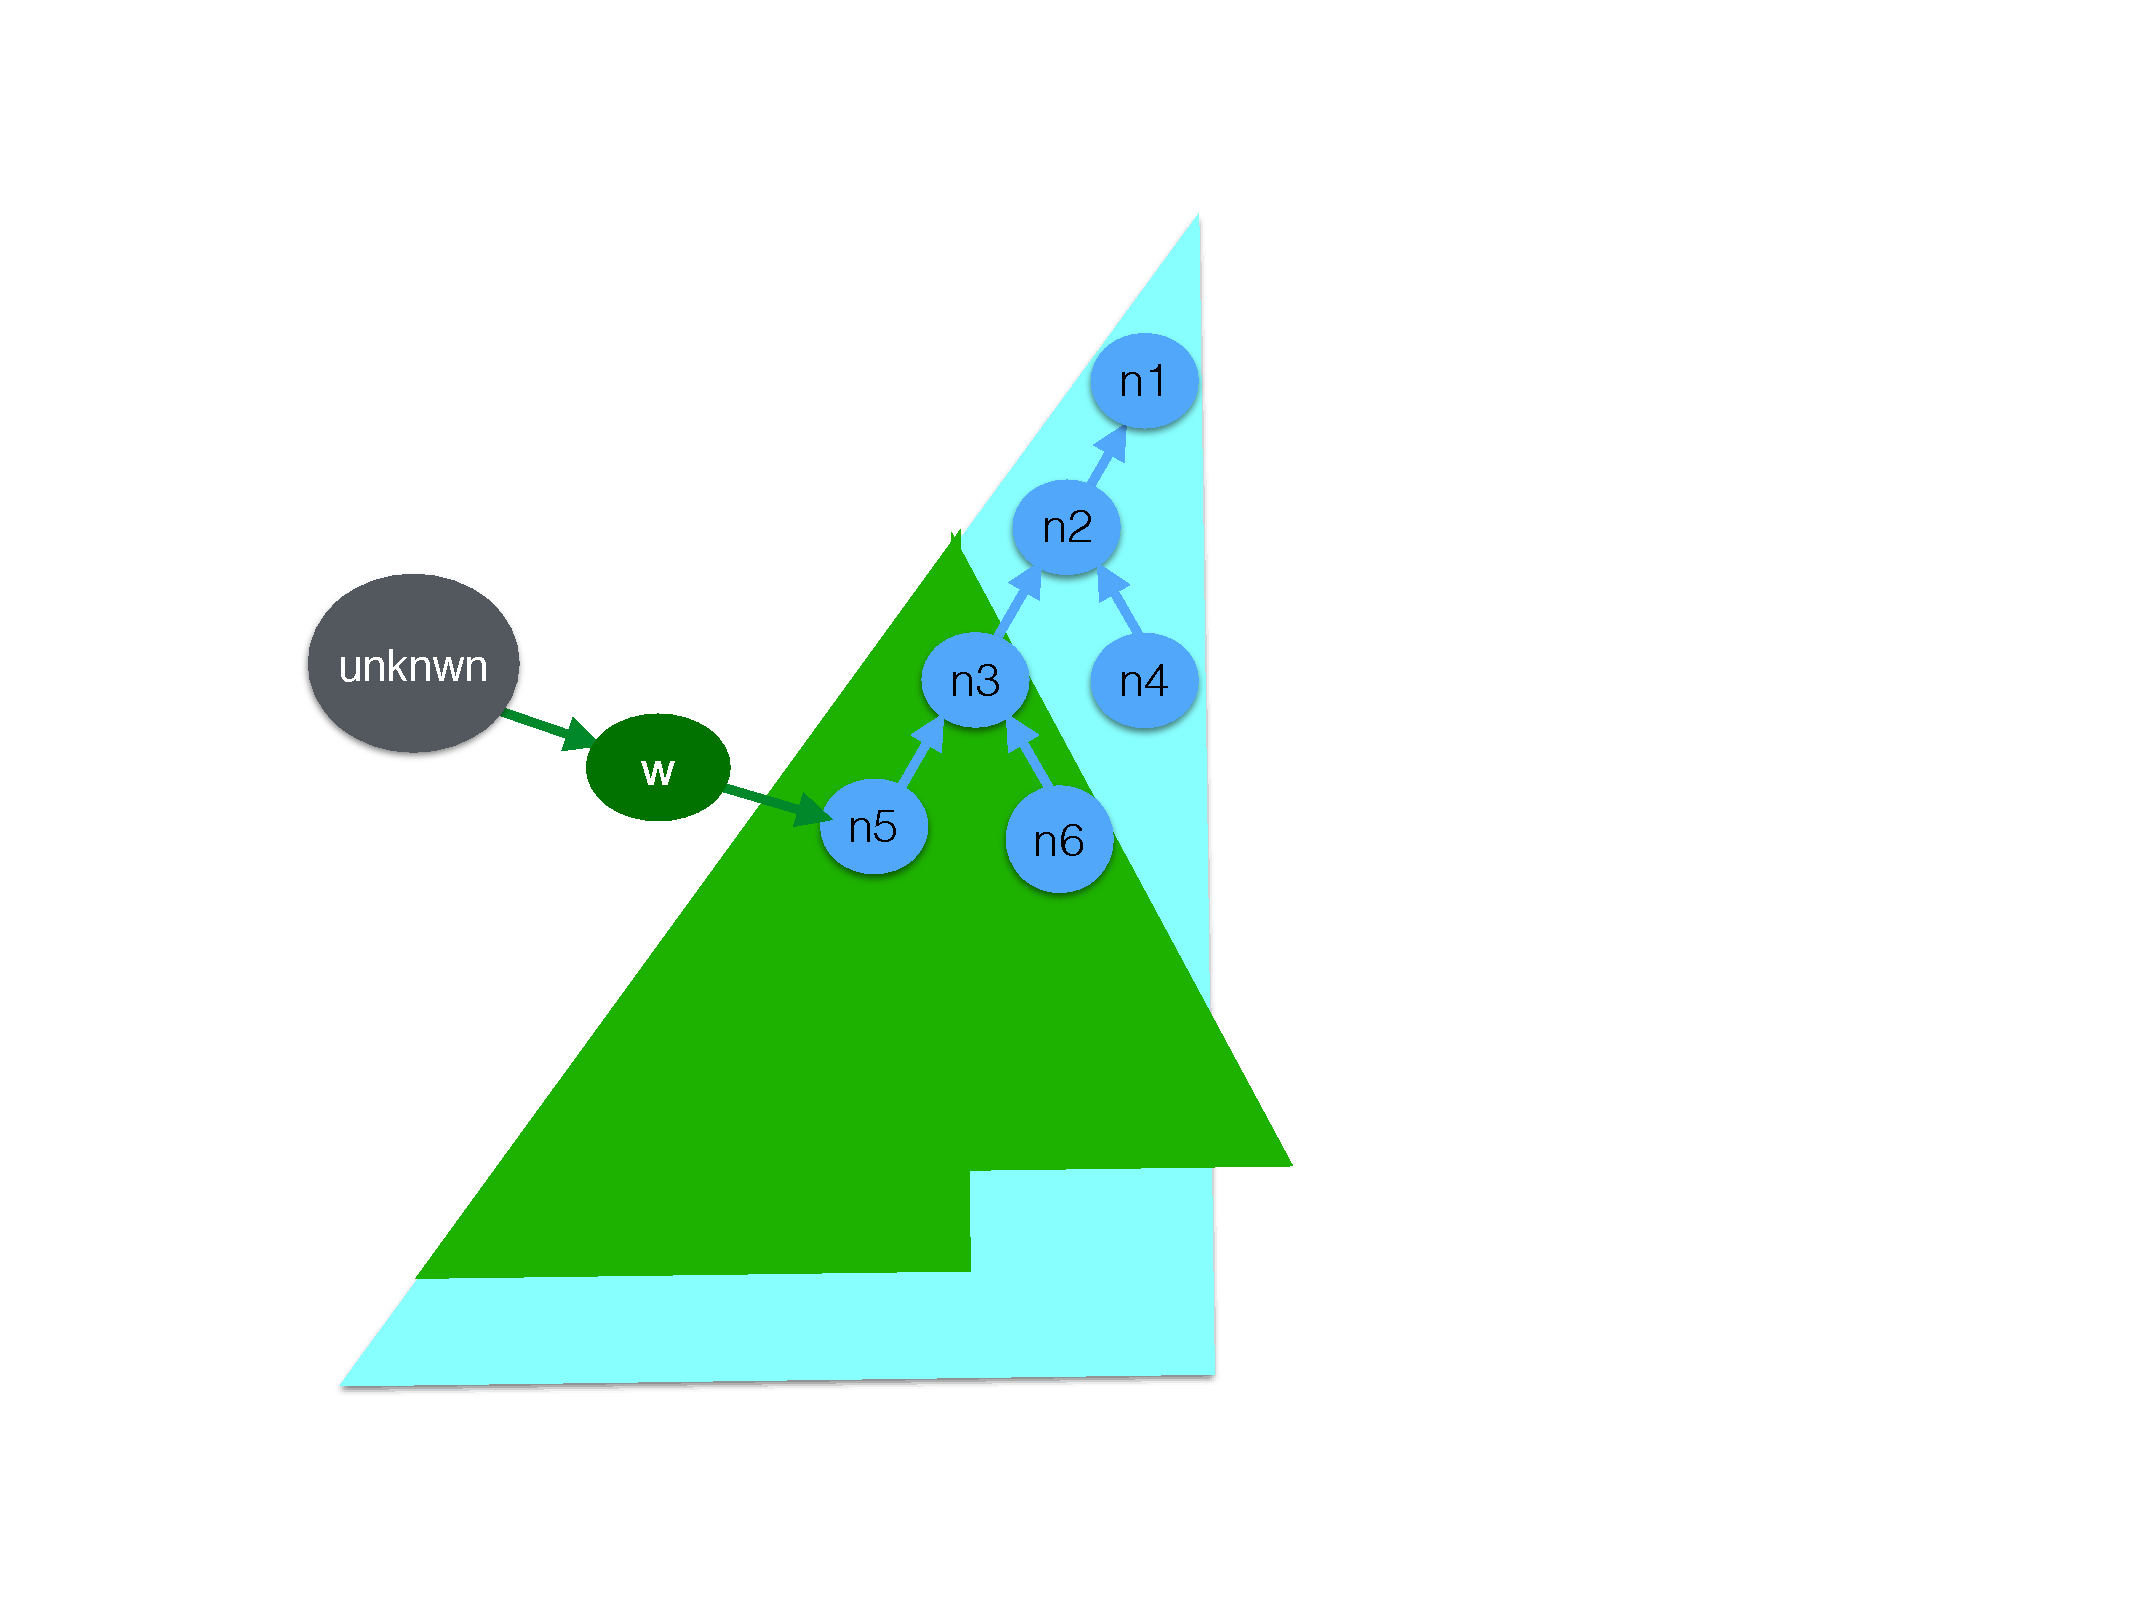
\includegraphics[width=\linewidth, trim=145  320 60 105,clip]{diagrams/DOM.pdf}
% x y z w
% y seems to eat up the bollom
% y=320 is good
% x eats space from left, if you increase it the diagram decreases from left
% w eats space from top, if you increase it the diagram decreases from top
% w=100 is good
%\includegraphics[page=3, width=\linewidth, trim=150  270 40 150, clip]{diagrams/snmalloc.pdf}\sdcomment{I think we need to change the diagram so that it says small slab.}
\strut \\
\strut \\

\end{minipage}
\end{tabular}
 \vspace*{-4.5mm}
\caption{\prg{Wrapper}s protecting \prg{Node}s }
\label{fig:WrapperUse}
\end{figure}

Even though we know nothing about the \prg{unknown} object or
its \prg{untrusted} function, and even though the call gives
to \prg{unknown} access to \prg{w}, which in turn has transitively
access to all \prg{Node}-s in the tree, we know that %the call to
the \prg{untrusted} function is guaranteed not to line 10 will not
affect the \prg{property} fields of the nodes \prg{n1}, \prg{n2},
and \prg{n4}.  Thus, the assertion on line 12 is guaranteed to
succeed.  The question is how do we specify \prg{Wrapper}, so as to be
able to make such an argument. %prove this assertion.

A specification of the class \prg{Wrapper} in the traditional
style, \eg \cite{Leavens-etal07} (\cf appendix \ref{DOM:traditional})
consists of pairs of pre- and post- conditions for each of the
functions of that class. Each such pair gives a {\em sufficient}
condition for some effect to take place: for example the
call \prg{w.setProperty(i,prp)} where \prg{i} is smaller
than \prg{w.height} is a sufficient condition to modify \prg{property}
of the \prg{i}-th parent of \prg{w.node}. But we do not know what
other ways there may be to modify a node's \prg{property}.  A broken
wrapper could accidently permit access to nodes one or two levels
about the expected height due to off-by one errors. More seriously,
a malicious wrapper could offer a
back-door public accessor method that leaks the underlying DOM
object through the wrapper, return direct access to any of the
other nodes in the DOM, or even to queue a task to
delete every property at midnight GMT on 29 March 2019. All of these errors are possible while
preserving the pre- and post- conditions expected of a \prg{Wrapper}. 
What is needed here is some way to specify the \emph{necessary
conditions}
under which some change could be made: if some external client is to
change a node's property, then  that client must have either direct
access to a node in that DOM tree, or indirect access via a wrapper
configured so that it can change the affected node.
Thus,
 \sdcomment{Shall we say the following, or does it break the flow?  
"Moreover, on line 10 we do not know which functions are called
on \prg{w}."
\kjx{I put that in and expanded on it. We need to explain the issues I think}
I do not see where it is}

% I think the below should be clear by niw
% In this work, we propose \emph{holistic specifications}, which
%describe the behaviour of an abstract data type as a whole, taking all
%possible method calls into account. Such holistic specifications
%emphasize the \emph{necessary conditions} for some effect to take
%place over the sufficient conditions as in traditional
%specifications. In our example:

\begin{quote}
The \emph{necessary} condition for the modification of \prg{nd.property} for some \prg{nd} of class \prg{Node}  is either access to some   \prg{Node} in the same tree, or  access to a \prg{w} of class \prg{Wrapper} where the \prg{w.height}-th parent of \prg{w} is an ancestor of \prg{nd}.
\end{quote}


With such a specification we can prove that the assertion on line 12
will succeed. Crucially, we can ensure that all future updates of
the \prg{Wrapper} class must continue to meet that specification,
guaranteeing the protection
of the \prg{Node} data. 
%
% Having justified the need for  necessary conditions in specifications, 
%
To give a flavour of \Chainmail, we use it  express the requirement from above:
%  This  gives us the opportunity to  demonstrate primitives for time ($\Future{\_}$) and authority ($\Changes{\_}$ and $\Using {\_} {\_}$).
 % and   more traditional relations between objects ( $\prg{nd}.\prg{parnt}^k\!=\! ...$):
% $\strut$ 
\vspace{.1cm}

\noindent
% \begin{quote}
$\forall \prg{S}:\prg{Set}.\forall \prg{nd}:\prg{Node}.\forall \prg{o}:\prg{Object}.$\\
$[\ \ {\Using{\Future {\Changes {\prg{nd.property}}}}  {\prg{S}}}$ \\
$\strut  \ \ \longrightarrow$\\
$\strut \ \ \ \exists \prg{o}.[\ \prg{o}\in\prg{S}\ \ \wedge\ \ \neg(\prg{o}:\prg{Node})\ \ \wedge\  \ \neg(\prg{o}:\prg{Wrapper})\ \ \ \wedge \  $\\
$ \strut\ \ \  \ \ \ \ \ \ \ \ [\ \exists \prg{nd}':\prg{Node}. \CanAccess{\prg{o}}{\prg{nd}'}\  \ \ \  \vee$\\
$ \strut\ \  \ \  \ \  \ \ \ \ \ \ \ \exists \prg{w}:\prg{Wrapper}.\exists k\!:\!\mathbb{N}.
% $\\ $ \strut \ \ \ \ \ \ \ \ \ \ \ \ \ \ \ \ \  \ \ \
  (\ \CanAccess{\prg{o}}{\prg{w}}  \ \wedge\ \prg{nd}.\prg{parnt}^k\!=\!\prg{w.node}.\prg{parnt}^{\prg{w.height}}) \ \ \ ]\ ]$\\
$ ]$
% \end{quote}

\vspace{.1cm}

% \noindent
That is, if the value of \prg{nd.property} is modified
($\Changes{\_}$) at some future point ($\Future{\_}$) and if reaching
that future point involves no more objects than those from set \prg{S}
(\ie ${\Using{\_} {\prg{S}}}$), then at least one (\prg{o}) of the
objects in \prg{S} is not a \prg{Node} nor a \prg{Wrapper},
and \prg{o} has direct access to some node
($\CanAccess{\prg{o}}{\prg{nd}'}$), or to some wrapper \prg{w} and
the \prg{w.height}-th parent of \prg{w} is an ancestor of \prg{nd}
(that is,
$\prg{parnt}^k\!=\!\prg{w.node}.\prg{parnt}^{\prg{w.height}}$).
% It is important to clarify what we mean by ``access''. 
Definitions of these concepts appear later
(Definition \ref{def:valid:assertion}), but note that our ``access''
is intransitive: $\CanAccess x y$ holds if either \prg{x} has a field
pointing to \prg{y}, or \prg{x} is the receiver and \prg{y} is one of
the arguments in the executing method call.
 
In the next sections we proceed with a formal model of our model. In the appendix we discuss more -- and simpler -- examples.
We chose the DOM for the introduction, in order to give a flavour of the \Chainmail features.
 


\section{Wrappers -- traditional Specification}
\label{DOM:traditional}
The figure needs some beautification

\begin{figure}[htb]
\begin{lstlisting}
class Wrapper(nd,hgt){

  fld node=nd;
  fld height=hgt;

  func setPropety(i,prp)
  // PRE:  true
  // POST:
  //     (  i not a number or i>this.height ) --> modifies nothing  
  //     &&
  //     i<=this.height -->  (  modifies = { this.node.parent^i.property }
  //                          &&
  //                          this.node,parent^i.property == prp )
  {
    if (i>height){     return     } 
    else  
    {  nd=node;  
       while (i>0){   nd=nd.getParent();  i--;    };
        nd.setProperty(prp); }
  }    
  func getChild(i)
  // PRE:  true
  // POST:  modifies: nothing
  // RETURNS: i-th child of this
  
  {    Wrapper(node.getChild(i),   height+1);   }                           
}
\end{lstlisting}
 \vspace*{-7mm}
\caption{\prg{Wrapper} specification}
\label{fig:WrapperSpec}
\end{figure}

In Figure \ref{fig:WrapperSpec} we  outline a specification of the class \prg{Wrapper} in the ``traditional style''. Each function has a pore and a post conditon. Because the functions may be called by any, unchecked code, the preconditions are not stronger than \prg{true}. The functions need to behave correctly under all possible circumstances.  The post-condition of \prg{setPropery} guarnatees that if the argument is not a number or if it is larger than the \prg{height} of the wrapper, then nothing is modified. If on the other hand, the argument is smaller or equal to the \prg{height}, then the \prg{property} of the \prg{i}-th parent will be set to \prg{prp}, and nothing else will be modified.


\section{Example -- ERC20}
 
 ERC20~\cite{ERC20} is a widely used token standard which describes the 
 basic functionality expected by any    Ethereum-based token contract. 
 It issues and keeps track of participants' tokens, and supports the  transfer
 of tokens between participants. 
%
%
%An important question, therefore, is to identify the precise circumstances under which a transfer of tokens may take place.
%The answer is that 
Transfer of tokens 
 can   take place only provided that  there were sufficient tokens in the
 owner's account, and that
 the transfer was instigated by the owner, or by somebody authorized
 by the owner.

We specify this in \Chainmail as follows:
A decrease in  a participant's \prg{balance} 
%(\ie  $\prg{e}.\prg{balance}=...\, \wedge\, \Next{\prg{e}.\prg{balance}=...}$)
can only be caused by a transfer instigated by the 
account holder themselves\\ (\ie $\Calls {\prg{p}} {\prg{transfer}} {...} {...}$), or by
an authorized transfer instigated by another participant $\prg{p}''$  (\ie $\Calls {\prg{p}''} {{\prg{transferFrom}} } {..} {..}$) who 
has authority for more than the tokens spent (\ie  $\prg{e}.\prg{allowed}(\prg{p},\prg{p}'')\geq \prg{m}$)
 
\vspace{.15cm}
\noindent
% \strut \hspace{0.3cm} 
$\forall \prg{e}:\prg{ERC20}.\forall \prg{p}:\prg{Object}.\forall \prg{m},\prg{m}':\prg{Nat}.$\\
\strut \hspace{0.3cm} $[\ \ \prg{e}.\prg{balance(p)}=\prg{m}+\prg{m'}\ \wedge \ \Next{\prg{e}.\prg{balance(p)}=\prg{m}'}$ \\ %.\forall\prg{m}:\prg{Nat}.$\\
\strut \hspace{0.4cm} \ \ \ $\longrightarrow$\\
\strut \hspace{0.4cm} \ \ \ $\exists \prg{p}',\prg{p}'':\prg{Object}.$ \\
\strut \hspace{0.4cm} \ \ \  $[\ \  \Calls{\prg{p}} {\prg{transfer}}  {\prg{e}}  {\prg{p}',\prg{m}} \  \  \ \vee\, $\\
\strut \hspace{0.4cm} \ \ \   $\ \ \ \ \prg{e}.\prg{allowed}(\prg{p},\prg{p}'')\geq \prg{m} \ \wedge \ \Calls{\prg{p}''} {\prg{transferFrom}}  {\prg{e}}  {\prg{p}',\prg{m}}\       \  ]$\\
\strut \hspace{0.3cm} $] $
\vspace{.15cm}

\noindent
That is to say: if next configuration witnesses a decrease of \prg{p}'s balance by
 $\prg{m}$, then the current configuration was a call of \prg{transfer} instigated by
 \prg{p}, or  a call of \prg{transferFrom} instigated by somebody authorized by \prg{p}.
 The term $\prg{e}.\prg{allowed}(\prg{p},\prg{p}'')$,  means that the
ERC20 variable \prg{e} holds a field called \prg{allowed}   which maps pairs of participants to numbers; such
mappings are supported in Solidity\cite{Solidity}.
 
We now define what it means for $\prg{p}'$ to be authorized  to  spend 
up to \prg{m} tokens on  $\prg{p}$'s behalf: At some point in the
past,  \prg{p} gave authority to $\prg{p}'$  to spend   \prg{m}
plus the sum of  tokens
spent so far by $\prg{p}' $ on the behalf of \prg{p}. 

 
\vspace{.15cm}
\noindent
 $\forall \prg{e}:\prg{ERC20}.\forall \prg{p},\prg{p'}:\prg{Object}.\forall \prg{m}:\prg{Nat}.$\\
\strut \hspace{0.3cm} $[\ \ \prg{e}.\prg{allowed}(\prg{p},\prg{p}')=\prg{m} $\\
\strut \hspace{0.4cm} \ \ \ $\longrightarrow$\\
\strut \hspace{0.4cm} \ \ \  
     $\PrevId\langle\ \  \Calls{\prg{p}}  {\prg{approve}}  {\prg{e}} {\prg{p}',\prg{m}} $\\
      \strut \hspace{1.7cm} \ $\vee $\\
\strut \hspace{1.7cm} \  
     $    \prg{e}.\prg{allowed}(\prg{p},\prg{p}')=\prg{m}   
        \  \wedge\ $\\
\strut \hspace{1.5cm} \ \ \ \ \          
$  \neg   (\, {\Calls{\prg{p}'} {\prg{transferFrom}} {\prg{e}} {\prg{p},\_}   } \, \vee \, {\Calls{\prg{p}} {\prg{approve}} {\prg{e}} {\prg{p},\_} } \, ) $\\
      \strut \hspace{1.7cm}\  $\vee $\\
\strut \hspace{1.7cm}   \  $ \exists \prg{p}'':\prg{Object}.\exists\prg{m'}:\prg{Nat}.$\\
 \strut \hspace{1.7cm}\  $[\   
  \prg{e}.\prg{allowed}(\prg{p},\prg{p}')=\prg{m}+\prg{m}'  \, \wedge\,   {\Calls{\prg{p}'} {\prg{transferFrom}} {\prg{e}} {\prg{p}'',\prg{m}'}  }   ]$\\
\strut \hspace{0.4cm} \ \ \  \ \ \  \ \ \ \ \ $\rangle $\\
\strut \hspace{0.3cm} $]$
\vspace{.15cm}
 
In more detail\  $\prg{p}'$ is allowed to spend 
up to \prg{m} tokens on their behalf of $\prg{p}$, if in the   previous step either a)
 \prg{p} made the call \prg{approve} on \prg{e} 
with arguments $\prg{p}'$ and \prg{m}, or b)  
$\prg{p}'$ was allowed to spend  up to \prg{m} tokens for $\prg{p}$
and did not transfer any of \prg{p}'s tokens, nor did \prg{p} issue a fresh authorization,
or c) \prg{p} was authorized for $\prg{m}+\prg{m}'$ and spent $\prg{m}'$. 
  
  \vspace{.1cm}
 
 Thus, the holistic specification gives to account holders an
 "authorization-guarantee": their balance cannot decrease unless they
 themselves, or somebody they had authorized, instigates a transfer of
 tokens. Moreover, authorization is {\em not} transitive: only the
 account holder can authorise some other party to transfer funds from
 their account: authorisation to spend from an account does not confer
 the ability to authorise yet more others to spend also.
 
% \paragraph{Comparison with Traditional Specifications}
 
 With traditional  specifications, to obtain the "authorization-guarantee", 
one would need to inspect the pre- and post- conditions of {\em all} the functions
in the contract, and determine which of the functions decrease balances, and which of the functions 
 affect authorizations.
 In the case of the \prg{ERC20}, one would have to inspect all eight such specifications
 (given in appendix \ref{ERC20:appendix}), 
 where only five are relevant to the question at hand.
 In the general case, \eg the DAO, the number of   functions which are unrelated
 to the question at hand can be very large.
  
More importantly, with traditional  specifications, nothing stops the next release of the contract to add, 
\eg, a method which allows participants to share their authority, and thus
violate the "authorization-guarantee", or even a super-user from skimming 0.1\% from each of the accounts.



\section{Example -- DAO}
The DAO  {(Decentralised Autonomous Organisation)}~\cite{Dao}  is a famous Ethereum contract  which aims to support
collective management of funds,  and to place power directly in the
hands of the owners of the DAO
rather than delegate it to directors.
Unfortunately, the DAO was not robust:
a re-entrancy bug   exploited in June 2016 led  to a loss of   \$50M, and
a hard-fork in the  chain ~\cite{DaoBug}.
%
%In a similar style as that  of the ERC20 spec earlier,
%We can give a \Chainmail~specification
With holistic specifications  we can  write a succinct requirement that a
DAO contract should always be able to repay any owner's money.
Any contract which satisfies such a holistic specification cannot demonstrate the DAO bug.
 
Our specification consists of three requirements.
First, that the DAO always holds at least as 
much money as any owner's balance.
%  \james{ALL owners? or does that follow?} 
To express this we use 
the field \prg{balances} which is a mapping from participant's addresses to 
numbers. Such mapping-valued fields exist in Solidity, but they could
also be taken to be ghost fields~\cite{ghost}.
  
\vspace{.1cm}

\noindent
 \strut \hspace{0.5cm} $\forall \prg{d}:\prg{DAO}.\forall \prg{p}:\prg{Any}.\forall\prg{m}:\prg{Nat}.$\\
\strut \hspace{0.5cm} $[\ \ \prg{d.balances(p)}=\prg{m}  \ \ \  \longrightarrow  \ \ \ \prg{d}.\prg{ether}\geq \prg{m} \ \ ] $


\noindent
Second, that when an owner asks to be repaid, she is sent all her money.
\vspace{.1cm}

\noindent
 \strut \hspace{0.5cm} $\forall \prg{d}:\prg{DAO}.\forall \prg{p}:\prg{Any}.\forall\prg{m}:\prg{Nat}.$\\
\strut \hspace{0.5cm} $[\ \ \prg{d.balance(p)}=\prg{m}
 \ \wedge \ \Calls{\prg{p}}{\prg{repay}}{\prg{d}}{\_}  $\\
 $\strut \hspace{5.5cm}   \ \ \  \longrightarrow  \ \ \  \Future{\Calls{\prg{d}}{\prg{send}}{\prg{p}}{\prg{m}}}\ \ ] $  
\vspace{.1cm}

 

%\kjx{combined defn ensuring enough eth at the time repayment is made:\\
%\noindent
% \strut \hspace{0.5cm} $\forall \prg{d}:\prg{DAO}.\forall \prg{p}:\prg{Any}.\forall\prg{m}:\prg{Nat}.$\\
%\strut \hspace{0.5cm} $[\ \ \prg{d.balance(p)}=\prg{m}
% \ \wedge \ \Calls{\prg{p}}{\prg{repay}}{\prg{d}}{\_}  $\\
% $\strut \hspace{5.5cm}   \ \ \  \longrightarrow  \ \ \  \Future{\Calls{\prg{d}}{\prg{send}}{\prg{p}}{\prg{m}}
% \wedge \prg{d}.\prg{ether}\geq \prg{m}}\ \ ] $
%\vspace{.1cm}
%}
%
%\kjx{negative example for talk, upping funds not calling send:\\
%\noindent
% \strut \hspace{0.5cm} $\forall \prg{d}:\prg{DAO}.\forall \prg{p}:\prg{Any}.\forall\prg{m}:\prg{Nat}.$\\
%\strut \hspace{0.5cm} $\ \ \Calls{\prg{d}}{\prg{send}}{\prg{p}}{\prg{m}}
% \strut \ \ \  \longrightarrow  \ \ \  \prg{d}.\prg{ether}\geq \prg{m}$\\
% % SD thinks the last  \longrightarrow sgould be wedge
%  $\strut \ \ \  \longrightarrow  \ \ \  \prg{p.funds}
%  = \Prev{\prg{p.funds}} + \prg{m}$
%\vspace{.1cm}
%}


\noindent
\sd{Third, that the balance of an owner is a function of its balance in the previous step,
or the result of it joining the DAO, or asking to be repaid \etc.}
 
\noindent
$\strut \hspace{0.5cm} \forall \prg{d}:\prg{DAO}.\forall \prg{p}.\forall:\prg{m}:\prg{Nat}.$\\
$\strut \hspace{0.5cm} [ \ \ \  \prg{d.Balance(p)}=\prg{m} \ \ \  \longrightarrow   
 \ \  \ \ 
  [ \  \ \Prev{\Calls{\prg{p}}{\prg{repay}}{\prg{d}}{\_}}\, \wedge\, \prg{m}=\prg{0} \ \ \ \ \vee $\\
$\strut \hspace{5.7cm}      
\Prev{\Calls{\prg{p}}{\prg{join}}{\prg{d}}{\prg{m}}}  \ \ \ \ \vee   $\\
 $\strut \hspace{5.7cm}  ... \  ]$ \\
%                         
%                         $ \left\{
%                            \begin{array}{ll}
%                             \prg{0}, & \hbox{if}\ Prev(Call(\prg{p},\prg{d.repay(),\_})    \\
%                             \vee
%                             \\
%                             \prg{m},  & \hbox{if}\  Prev(Call(\prg{p},\prg{d.join(),m}))   \\
%                             ..., & ...
%                           \end{array}
%                         \right.    $\\
$\strut \hspace{0.5cm} ] $
  


More cases are needed to reflect the financing and repayments of proposals, but they can be expressed with the concepts described so far.


 

\noindent
The requirement that \prg{d} holds at least \prg{m} ether precludes the DAO bug,
in the sense that  any contract satisfying that spec cannot exhibit  the  bug:   a contract
which satisfies the spec  is guaranteed to always have enough money to satisfy all \prg{repay} requests.
This guarantee  holds, regardless of how many functions there are in the DAO.
In contrast, to preclude the DAO  bug with a classical spec, one would need to write a spec for each of the
DAO functions (currently 19), a spec for each function of the auxiliary contracts used by the DAO,
and then study their emergent  behaviour.

These 19 DAO functions   have several different concerns:
who may vote   for a proposal, who is eligible to submit a proposal,
how long the consultation period is for deliberating a proposal, what
is the quorum, how to chose curators, what is the value of a token,
Of these groups of functions, only  a handful affect the balance of a
participant. Holistic specifications allow us to concentrate on aspect of DAO's behaviour across \emph{all} its functions.
 


\section{Example -- Purse and Mint}
take from our earlier works

In two versions: one where there is a ledger inside the Mint, and one where the Mint has no path to the Purses. This will serve to demonstrate how \prg{internal} is supposed to work.

\section{Example -- Membrane}

TODO - take from ShuPeng's thesis
}
 \newpage
% \small{
  \bibliographystyle{plain}
\onecolumn{
 \bibliography{Case,more}


}
\end{document}

THE rest
\begin{definition}[Time, Permission, Authority,  and Space ]
\label{def:permission}
Given a module $\M$, identifiers \code{x} and \code{y}, expression $\sE$, and runtime configuration $\sigma$, and a set of addresses $S$,
we define validity of the assertions   .... as follows:

\begin{itemize}
\item
$\M,\sigma \models  \Future \A$\ \ iff\ \  $\exists \sigma'.\, [\ \ \M,\sigma \leadsto^* \sigma' \ \wedge \ \M,\sigma' [\overline{x \mapsto \sigma(x)}]\models \A, \mbox{ where } \overline{x}=Free(\A)\   ]$.
\item
$\M,\sigma \models  \Past \A$\ \   iff\ \  $\exists \sigma_1,....\sigma_n, k\!\in\![1..n-1).\ [ \Initial {\sigma_1}\  \wedge\ \sigma_n=\sigma\ \wedge\ \forall i\!\in\![1..n).\ \M,\sigma_i\leadsto  \sigma_{i+1}  $\\
\strut \hspace{5.7cm} $\ \wedge \  \ \M,\sigma_k[\overline{x \mapsto \sigma(x)}]\models \A, \mbox{ where } \overline{x}=Free(\A)\  ]$.


\item
 $\sigma\!\mid_S$ denotes a {\em restriction} of $\sigma$ to the objects from the set $S$. That is, the domain of
 the heap in $\sigma\mid_S$ is $S$, and otherwise,  $\sigma\mid_S$ is identical to $\sigma$. An example appears in figure \ref{fig:DiagramRestricted}.
 \item
$\M,\sigma  \models \Using{\A}{\prg{S}}$  \  \ iff \ \
  $ \M,\sigma\!\mid_S\, \models \A $, where   $S=\interp {\prg{S}} {\M,\sigma} $.
 \item
 $\M,\sigma  \models \Calls {m}$ \ \ iff \ \ the method call in the current frame in $\sigma$ is
 \prg{m}\footnote{We will express this precisely  when we have the full definition of $\sigma$}
\end{itemize}
\end{definition}

\begin{figure}[btph]
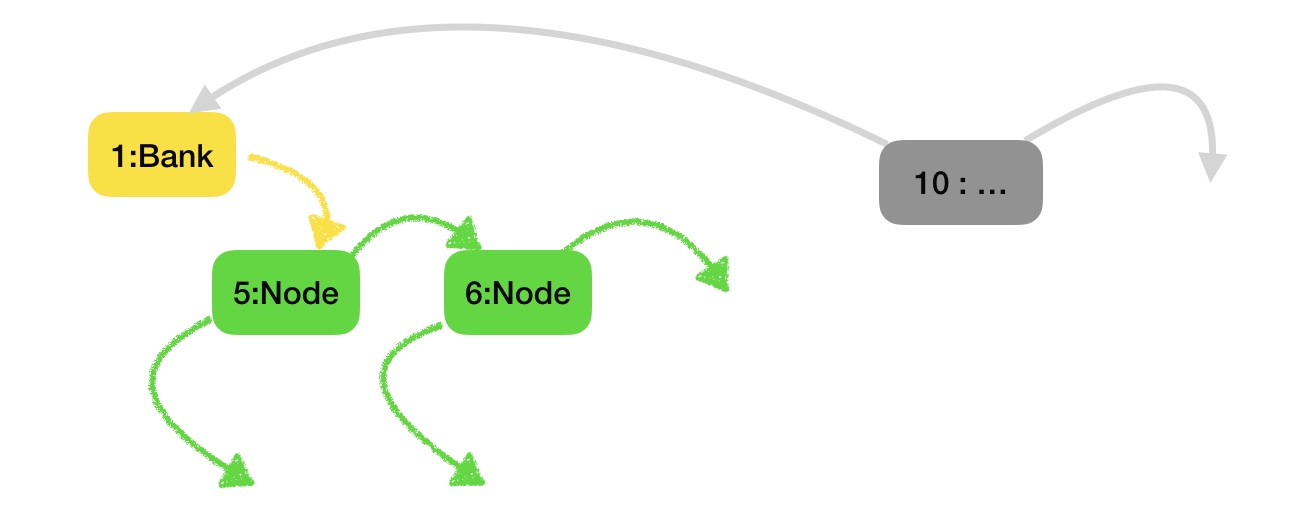
\includegraphics[width=10cm,height=4cm]{diagram2}
 \caption{Configuration from Fig. \ref{fig:Diagram} restricted to witness \{ \prg{1}, \prg{5}, \prg{6}, \prg{10} \}}
  \label{fig:DiagramRestricted}
  \end{figure}

Note that $\CanAccess{\prg{x}}{\prg{y}}$ is reflexive but  not transitive and not symmetric.

Also note the difference between $\Using{(\Future{\A})}{\prg{S}}$ and $\Future{(\Using{\A} }{\prg{S}})$.
For example,  the assertion  $\Using{(\Future{\prg{x}.\prg{f}=\prg{z}})}{\prg{S}}$ expresses that the current execution
leads to a future configuration  where
$\prg{x}.\prg{f}=\prg{z}$ will hold, and that the set \prg{S} suffices to witness this execution, while the assertion
$\Future{(\Using{{\prg{x}.\prg{f}=\prg{z}} }}{\prg{S}})$  expresses that the current execution
leads to a future configuration   where
$\prg{x}.\prg{f}=\prg{z}$ will hold and where  the set \prg{S} suffices to witness
that fact.
For example, take a configuration $\sigma$ where variable \prg{x} maps to some object \prg{31}, and where \prg{31} has a field \prg{f}
pointing to \prg{32}, and \prg{32} has a field \prg{f}
pointing to \prg{33}, and variable \prg{z} maps to  \prg{33}. Assume also that the expression to be executed in $\sigma$ starts with
\prg{x.f}=\prg{x.f.f}. Then we have that
$\M,\sigma  \models \Future{(\Using{{\prg{x}.\prg{f}=\prg{z}} }{\{\prg{x},\prg{z}\}})}$,
but
$\M,\sigma  \not\models \Using{(\Future{\prg{x}.\prg{f}=\prg{z}})}{\{\prg{x},\prg{z}\}}$.
On the other hand
$\M,\sigma  \not\models \Using{(\Future{\prg{x}.\prg{f}=\prg{z}})}{\{\prg{x},\prg{x}.\prg{f},\prg{z}\}}$

In general, for all $\M$ and $\sigma$, we have that
 $\M,\sigma \models  \Using{(\Future{\A})}{\prg{S}}$ implies $\M,\sigma \models \Future{(\Using{\A} }{\prg{S}})$, and that
 $\M,\sigma \models \Future{(\Using{\A} }{\prg{S}})$ implies that there exists a set $\prg{S}'$ such that
 $\M,\sigma \models  \Using{(\Future{\A})}{(\prg{S}\cup\prg{S'})}$.

\vspace{.2in}
We will prove that

\begin{lemma}[Preservation of validity and module linking]

$\M,\sigma \models \A$  \ \ \ then\ \ \ \   for all $\M'$ with $\M\link\M'$ is defined:\ $\M\link\M',\sigma \models \A$.
\end{lemma}




\subsection{Invariants}

We define below the meaning of invariants.\footnote{This part is as we had defined previously, with two simplifications: a) we do not need to worry about the $\obeys$-predicate here, and b) we do not distinguish the names of the classes and the names of participants in interfaces.}
The assertion $\M   \models\  \A$ requires that  the assertion $A$ is satisfied
in all reachable states.

\begin{definition}[Invariants]
\label{def:invariant}
\noindent
For a module $\M$  and assertion $\A$ we define:\\

 \begin{itemize}
 \item
$\M   \models\  \A$\ \ \  iff\ \ \ \
% $\strut\SP\SP$
$\forall \M'.\, \forall \sigma\!\in\!\Arising(\M'*\M).\ \M'*\M,\sigma \models \  \A$
 \end{itemize}
\end{definition}

The use of the set of configurations from $\Arising(\M'*\M)$ reflects that policies
 need to hold in an {\em open} world, where
we link against {\em any} module $\M'$,
about which we know nothing.

\subsection{Implication and equivalence}

\begin{definition}
\label{def:impl:equiv}
\noindent
For a module $\M$  and assertions $\A$  and $\A'$, we define strong equivalence and implication ($\equiv$ and $\sqsubseteq$), as well
as   weak equivalence and implication ($\approxeq$ and $\weakImplies$)  as follows:


 \begin{itemize}
\item
$\M   \models\  \A \strongImplies \A'$  \ \ \ \ iff \ \ \ \
$\forall \M'.\, \forall \sigma\!\in\!\Arising(\M'*\M).[\ \ \  \M'*\M, \sigma \models \A \  \ \  \longrightarrow\  \ \  \M'*\M, \sigma \models \A'\ \ \ ]$
 \item
$\M   \models\  \A \equiv \A'$ \ \ \ \ iff \ \ \ \
$\M   \models\  \A \strongImplies \A'\ \  \wedge \ \  \M   \models\  \A' \strongImplies \A$
%$\forall \M'.\, \forall \sigma\!\in\!\Arising(\M'*\M):\ \ \  \M'*\M, \sigma \models \A \  \ \longleftrightarrow\   \ \M'*\M, \sigma \models \A'$
\item
$\M   \models\   \A \weakImplies \A'$  \ \ \ \ iff \\ \ \ \ \ \ \
\strut  \hspace{1cm}  $\forall \M'.\, \forall \sigma\!\in\!\Arising(\M'*\M).\,\M'*\M, \sigma \models \A$ \  \ \  $\longrightarrow$\  \ \
$\forall \M'.\, \forall \sigma\!\in\!\Arising(\M'*\M).\,\M'*\M, \sigma \models \A'$
\item
$\M   \models\  \A \approxeq \A'$   \ \ \ \ iff \ \ \ \ \
$ \M  \models  \A \weakImplies \A' \   \ \wedge\   \  \M  \models  \A' \weakImplies \A$
 \end{itemize}
\end{definition}

The definitions from above are applicable to the empty module, eg  $\models\  \A \equiv \A'$ iff   all modules $\M$ satisfy $\M \models\  \A \equiv \A'$.
The following properties hold:

\begin{lemma}
For all modules \M, assertions \A and \A':

 \begin{itemize}
 \item
$\M   \models\  \A \equiv \A'$  \ \ \ implies \ \ \  $\M   \models\  \A \simeq \A'$
\item
$\M   \models\  \A \strongImplies \A'$  \ \ \ \ implies  \ \ \ \
$\M \models \A \weakImplies \A$
\item
$\M \models   \Using{(\Future{\A})}{\prg{S}}\ \strongImplies\ \Future{(\Using{\A} }{\prg{S}})$
\item
$ \M \models\  \Future{\A}\rightarrow \A' \  \  \weakImplies \ \ \A\rightarrow\Past{\A'}$
\item

 \end{itemize}
\end{lemma}

\paragraph{Space-Monotonicity}\footnote{Not sure how useful this concept is}

\begin{definition}[Space-Monotonicity]
We call an assertion $\A$ {\em space-monotonic} in $\M$, iff for all set expressions $\prg{S}$ and  $\prg{S}'$,
  % $\M,\sigma\models ( \prg{S} \subseteq \prg{S}'\ \wedge\  \Using{\A, \prg{S}}) \ \strongImplies\  (\Using{\A, \prg{S'}})$
%\end{definition}\footnote{If we unfold the definitions, we obtain that
% $\A$ is space-monotonic in $\M$, iff for all set expressions $\prg{S}$ and  $\prg{S}'$
 and all $\sigma\in\Arising({\M})$:
 \\
  If  $\M,\sigma\models  \prg{S} \subseteq \prg{S}'$ and $\M,\sigma\models  \Using{\A} {\prg{S}}$, then
$\M,\sigma\models  \Using{\A}{ \prg{S'}}$
\end{definition}

We prove space monotonicity for some assertions

\begin{lemma}[Space-Monotonicity for change and access]
$ ~ $

\begin{itemize}
\item
${\Changes \sE} $ is space-monotonic.
\item
$\CanAccess {\prg{x}}{\prg{y}}$ is space-monotonic.

\end{itemize}
\end{lemma}

Not all assertions  are not space-monotonic. E.g. $\forall a:\prg{Account}.\prg{a.balance}\geq 3$ is not space-monotonic.


The following lemma would be nice to have -- otherwise we will need to change the definition of monotonicity.

\begin{lemma}[Space-Monotonicity and module linking]
If $\A$ is space-monotonic with $\M$, then it is also space-monotonic with $\M*\M'$.
\end{lemma}


 \section{Specifications for Robustness Policies}

 We now use the concepts introduced in the earlier sections to specify various robustness policies

 \subsection{Specification of \Pol 2  and   \Pol 4}

We    give a formal definition of \Pol 2 and  \Pol 4, using the concepts defined earlier in  Definition \ref{def:permission}: %

\begin{definition}
\label{def:pol2}
We define  what it means for an object \prg{o} to be internal to a bank's data structure, an then define \Pol 2  and   \Pol 4  as follows:

%  \noindent
$\prg{Internal}(\prg{b})$ \ \  $\triangleq$ \ \
$\{\ \prg{o}\ \mid\  \prg{b}:\prg{Bank}\ \ \wedge \ \ (\ \prg{o} = \prg{b}\ \ \vee\  \ \prg{o}:\prg{Account}\wedge \prg{o}.\prg{myBank}=\prg{b}$\\
\strut \hspace{7.3cm} $\ \ \vee\ \ \ \exists k. \ \prg{b}.\prg{ledger}.\prg{next}^k = \prg{b})\ \ \ \ \}$


$\prg{Internal}'(\prg{a})$ \ \  $\triangleq$ \ \
$\{\ \prg{o}\ \mid\  \prg{a}:\prg{Account}\ \ \wedge \ \
 \prg{a}.\prg{myBank} :\prg{Bank}\ \wedge\  \prg{o}\in \prg{Internal}(\prg{b})\ \}$


 \vspace{.2cm}

  \Pol 2\ \  $\triangleq$ \ \
  $\forall \prg{b}.\forall \prg{S}.
  [ \ \  \prg{b}:
  \prg{Bank}\ \wedge\ \prg{this}\neq\prg{b}\ \wedge\ \ \Using{(\Future\Changes{\prg{b.currency}})}{\prg{S}} \ \ \ \ \longrightarrow \ \  $\\
   \strut $~ $ \ \ \ \hspace{1.7in}  \hfill
 $\exists \prg{o}. \ [ \ \
  \prg{o}\in \prg{S}\   \wedge\  \CanAccess{\prg{o}}{\prg{b}}\ \wedge\     \prg{o}\notin\prg{Internal}(\prg{b})  \ \ ]\ \ ]$


 \vspace{.1cm}
% \noindent
    \Pol 4\ \  $\triangleq$\ \ $\forall \prg{a}.\forall \prg{S}.\ [ \ \  \prg{a}:\prg{Account}\   \wedge\   \prg{this}\neq\prg{a} \ \wedge\ \Using{(\Future\Changes{\prg{a.balance}})}{\prg{S}}\ \ \   \
    \longrightarrow$ \\
 $\strut \hspace{3.9cm} \hfill \exists \prg{o}.\ [\, \prg{o}\in \prg{S}\ \wedge \ \CanAccess{\prg{o}}{\prg{a}}\ \wedge  \ \prg{o} \notin\prg{Internal}'(\prg{a}) \ ] \ \ \ \ ]$

\end{definition}

\paragraph{Discussion}
In other words, \Pol 2  mandates that the elements of the data structure (ie the elements from $\prg{Internal}(\prg{b})$) cannot be used (are not sufficient) to  change the currency of the bank. If a computation takes place inside the set \prg{S}, and {\em in the current state} in \prg{S}
all accesses to the bank go through elements of the data structure (ie the \prg{Account} objects),\footnote{Say why we can ignore \prg{Node} objects} then we have a guarantee that the computation will not affect the currency.
For example, if a computation takes place in the context of objects \prg{1}, \prg{2}, \prg{3}, \prg{4}, \prg{5}, \prg{7}, \prg{20} and \prg{21}, and the current receiver is no \prg{1}, then we have a guarantee that the currency of \prg{1} will not be affected. So, even through \prg{1} is involved in the computation, because there is no {\em external} access to it, we have a guaratee that the method \prg{makeAccount} will not be called on it.

An alternative way of expressing \Pol 2 is as follows:


 \Pol 2\ \  $\equiv$ \ \
  $\forall \prg{b}.\forall \prg{S}.
  [ \ \  \prg{b}:
  \prg{Bank}\ \wedge\   \prg{b}\neq\prg{this}\ \wedge\  \forall \prg{o} \in \prg{S}.\, [\ \prg{o}\in\prg{Internal}(\prg{b}) \ \vee\  \neg  \CanAccess{\prg{o}}{\prg{a}}  \ \ ]$
\\ \hfill \strut $~   \ \ \ \hspace{1.7in}  \  \ \longrightarrow \ \ \ \neg(
 \Using{(\Future\Changes{\prg{b.currency}})}{\prg{S}})\   \  \ \ ]$

\vspace{.01in}
% TO\_DO: discuss the difference between  $\Using{(\Future\Changes{\prg{b.currency}})}{\prg{S}})$, and
% $\Future{(\Using{\Changes{\prg{b.currency}}{\prg{S}})}}$.

\vspace{.01in}
\Pol 2  guarantees
that if an object \prg{o}$\neq$\prg{b} may affect the value of \prg{b.Currency} only if the  objects
involved in the process of affecting the value of \prg{b.Currency}  include at least an object $\prg{o}'$
which had direct access to \prg{b}, and
whose class is  not  \prg{Account}. Stated positively, this policy mandates
that exporting an \prg{Account} to an environment will not affect the \prg{Currency} of \prg{b}.
In other words,
\prg{Account}s protect the integrity of the \prg{Bank}'s currency.


In more detail, by applying  Definition \ref{def:invariant} on Definition \ref{def:pol2}, the  meaning of policy \Pol 2
  is, that a runtime configuration $\sigma$ satisfies  \Pol 2  if whenever the current receiver in $\sigma$
 is not a \prg{Bank} object, and the execution of $\sigma$ leads to another runtime configuration $\sigma'$
 with a different value for \prg{b.Currency}, then the objects involved in the execution from
 $\sigma$ to $\sigma'$ include at least one object which had direct access to \prg{b}.
 Note that this direct access needs to exist at the beginning of   the execution, \ie at $\sigma$.
 Formally:

 \noindent
 $\M, \sigma \models  \Pol 2$\\$ \strut \ \ \ \  \ \  \longleftrightarrow $\\
 $\forall \prg{b}.\forall S.\ [ \ \ \ \ \M, \sigma \models \prg{b}:\prg{Bank}\ \wedge\
 \sigma(\prg{b})\neq \ \sigma(\prg{this}) $\\
 $\strut \hspace{2.1cm}  \wedge \
 \ \exists\sigma'.(\ \ \ \ \M, \sigma\mid_S \leadsto^* \sigma'\
\ \wedge\ \interp {\prg{b.Currency}}{\M,\sigma}\neq \interp {\prg{b.Currency}}{\M,\sigma'[\prg{b}\mapsto\sigma(\prg{b})]}\ )$\\
$\strut \hspace{4.7cm} \longrightarrow$ \\
 $\strut \hspace{2.7cm}  %\exists \prg{o}. (\ \  \sigma(\prg{o}) \!\!\in\!\!\prg{S}\ \
 \exists \prg{o}. (\ \ \prg{o} \!\in\!S\ \
  \wedge \ \ \M, \sigma \models \CanAccess{\prg{o}}{\prg{b} }\ \wedge \  \prg{o}\notin \prg{Internal}(\prg{b}) \   \ ) \ \ \ \ \ \ \  ]$



\subsection{Specifying  "no leaks"}

This is a family of guarantees that Dean seemed especially interested in, when we discussed in March in London.
For the particular example, we want to express that

\begin{description}
\item[\Pol 7]
The \prg{Bank} does not leak out of the \prg{Bank}/\prg{Account} system
%\item[Pol\_7]
%The \prg{Accounts} do  not leak out of the \prg{Bank}/\prg{Account} system
\end{description}

And we give a formal specification

\begin{definition}[Banks do not leak]
\label{def:bankNoLEak} We define \Pol 7 as follows:

\Pol{7}\ \  $\triangleq$\ \ $\forall \prg{b}.\forall \prg{S}.\ [  \ \ \prg{b}:\prg{Bank}\ \wedge\  \prg{o}:\prg{Object}\  \wedge\   \neg(\CanAccess{\prg{o}}{ \prg{b}})\ \wedge\   \Using {(\Future{\CanAccess {\prg{o}}{\prg{b}}})} {\prg{S}} $
 \\  $\strut$ \hspace{4cm}
  $\longrightarrow$
 $\strut \hspace{0.5cm}  \exists \prg{o}'.\ [\, \prg{o}'\in \prg{S}\ \wedge \  \CanAccess{\prg{o}'}{ \prg{b} }\ \wedge\   \prg{o}' \notin \prg{Internal}(\prg{b}) \, ) \ ] \  \  \ \  ]$

%\hspace{.1cm}
%{\bf {Pol\_8}}\ \  $\equiv$\ \ $\forall \prg{o},\prg{b}, \prg{o}'\forall \prg{S}.\ [  \ \ \prg{b}:\prg{Bank}\ \wedge \prg{o}\in\prg{Internal}({\prg{b}})\ \wedge\  \prg{o}':\prg{Object}\ \ \neg(\CanAccess{\prg{o}'}{ \prg{o}})\ \wedge\   \Using {(\Future{\CanAccess {\prg{o}'}{\prg{o}}})} {\prg{S}} $
% \\  $\strut$ \hspace{4cm}
%  $\longrightarrow$
% $\strut \hspace{0.5cm}  \exists \prg{o}''.\ [\, \prg{o}''\in \prg{S}\ \wedge \  \CanAccess{\prg{o}''}{ \prg{o} }\ \wedge\   \prg{o}'' \notin \prg{Internal}(\prg{b}) \, ) \ ] \  \  \ \  ]$
\end{definition}

In other words, \Pol 7 guarantees that objects that are internal to the bank \prg{b} do not leak access to it.
In more detail: if   objects  \prg{o} and \prg{b} exist  now, and \prg{o} does not have direct access to \prg{b} now, but obtains
access to \prg{b} through some computation which involves objects from the set \prg{S}, then at least one  object  from \prg{S} has
now direct access to   \prg{b} and this object is not internal to \prg{b}.

\section{Adherence to Policies}
\label{section:Adherence}
In this section we will outline the proofs that particular modules adhere to their specifications.
This serves to demonstrate the practicality of our approach.
In particular we will show two different versions fo the \prg{Bank}/\prg{Account} example (sections \ref{section:Adherence:ModuleOne} and \ref{section:Adherence:ModuleTwo}, and we will prove that
both satisfy the policies \Pol 2, \Pol 4, and \Pol 7, while they differ in the definition of \prg{Internal}.
But before doing that, in section \ref{section:GeneralPropertiesExecution}, we will study some further properties of execution.


\subsection{General properties of execution}\footnote{Find better title?}
\label{section:GeneralPropertiesExecution}

We will first define some further predicates which reflect over the program execution and prove
some general properties of program execution.

We call a locations set, \prg{L}, an expression which denotes a set of addresses and field identifiers, \eg, $\{\ (\prg{b},\prg{ledger}), (\prg{b}.\prg{ledger},\prg{balance})\ \}$ is such a locations set.

\begin{definition}[Framing]
Take arbitrary module \M, assertion \A, , ...

\begin{itemize}
\item
\interp{\prg{L}}{\sigma,\M*\M'} = ....
\item
$ \sigma\mid _L$ ....
\item
$\M, \sigma \models \prg{L} \frames \prg{e}$\ \ \ \  \ iff \ \ \ \ \
$\forall \M'.\forall \sigma'\!\in\!\Arising({\M*\M'}). \forall L.$\\
\strut \hspace{1cm} $  [ \ \ L=\interp{\prg{L}}{\M,\sigma}\, \wedge\,
 \sigma\mid _L= \sigma'\mid_L \ \   \longrightarrow\ \ \   \interp {\prg{e}}{\sigma,\M*\M'}  =  \interp {\prg{e}}{\sigma',\M*\M'}
\ \ ]$
\item
$\M  \models \prg{L} \frames \prg{e}$\ \ \ \  \ iff \ \ \ \ \
$\forall \M'.\forall \sigma\!\in\!\Arising({\M*\M'}). \ \M'*\M, \sigma \models \prg{L} \frames \prg{e}$
\item
$\M, \sigma \models \prg{L} \frames\A $\ \ \ \  \ iff \ \ \ \ \
$\forall \M'.\forall \sigma'\!\in\!\Arising({\M*\M'}). \forall L.$\\
\strut \hspace{1cm} $ [ \ \ L=\interp{\prg{L}}{\M,\sigma}\, \wedge\,
\sigma\mid _L= \sigma'\mid_L \ \   \longrightarrow\ \ \   [\ \M*\M',\sigma \models \A   \ \longleftrightarrow\ \M*\M',\sigma' \models \A
\ \ ] $
\item
$\M  \models \prg{L} \frames \A$\ \ \ \  \ iff \ \ \ \ \
$\forall \M'.\forall \sigma\!\in\!\Arising({\M*\M'}). \ \M'*\M, \sigma \models \prg{L} \frames \A$
\end{itemize}

\end{definition}

NOTE\_TO\_SELF: we need to think about whether we also need to make \prg{L} self-framing.
Also, rethink whether we need to stick new modules $\M'$ to the whole thing.
--
Also, the sets are not equal -- they are isomorphic. We can deal with isomorphisms, but
it has a high notation penalty. Can we pretend that they are equal? hmhhhhh


And then we can prove that changes in the interpretation or the validity require a change in the frame:

\begin{lemma}[Change in the context of framing]
Take arbitrary module \M, assertion \A, such that  $\sigma\in\Arising({\M*\M'})$

\begin{itemize}
\item
If  $\M  \models \prg{L} \frames \prg{e}$, and
$\M'*\M, \sigma \models \Using{(\Future{\Changes{\prg{e}}})}{\prg{S}}$, \\
then there exists a pair $(\prg{e}',\prg{f})$ , with
$\M,\sigma \models (\prg{e}',\prg{f})\in \prg{L}$\footnote{Sophia, you need to check this bit  what if \prg{z}
there is no handle in \prg{L}, eg what if \prg{L} talks about anonymous objects
\eg \prg{L} = $\{ o \ \mid o.\prg{myBank}=\prg{b} \}$?Here $o$ is anonymous. Also, do we need $\M$ or $\M'*\M$?}
and $\M'*\M, \sigma \models  \Using{\Future{\Changes{\prg{e}'.\prg{f}}}}{\prg{S}}$

\item
similar for
$\M'*\M, \sigma \models \Using{\Future{\Changes{\A}}}{\prg{S}}$
\end{itemize}

\end{lemma}

\begin{figure}[tbp]
\begin{lstlisting}
 class Bank {
   private field ledger;   // a Node

   Bank( )
     { ledger = null; }
   fun makeAccount(amt)
     { account = new Account(this);
       ledger = new Node(account, amt, ledger);
       return account; }
   fun deposit(source, destination, amnt)
     { sourceNd = ledger.getNode(source)
       destinationNd = ledger.getNode(destination)
       if (sourceNd!=null && destinationNd!=null && sourceNd.balance>amt) then
          { < sourceNd.balance = sourceNd.balance-amt
              destinationNd.balance = destinationNd.balance+amt > }
        else
          { return }               }
 }

 class Account {
   private field myBank;  // a Bank

   Account(aBank)
     { myBank = aBank;  }
   fun sprout( )
     // create Account in same Bank with 0 balance
     { return this.myBank.makeAccount(0)  }
   fun deposit(source, amnt)
     // if destination is an Account in myBank,  and  source holds enough money,
     // then transfer amnt from source into receiver
     { myBank.deposit(source,this,amnt) }
 }

  class Node{
   field balance;     // the  money held in theAccount a number
   field next;        // the next node
   field theAccount;  // the account

   fun getNode(account)
     { if (theAccount==account) then
           { return this }
       elseif (next!=null)
           { next.getNode(account) }
       else
           {  return null }            }	
 }
\end{lstlisting}
\caption{\MOne: First version of the Bank example, in detail}
\label{fig:BankDetailedOne}
 \end{figure}


We now think a bit more about changes in accessibility. The predicate  $\Gives(\prg{x},\prg{y},\prg{z})$ expresses
that \prg{x} passed to \prg{y} access to \prg{z}.

\begin{definition}[Giving]
For arbitrary module \M and $\sigma$, we define:

\begin{itemize}
\item
$\M,\sigma  \models \Gives(\prg{x},\prg{y},\prg{z})$\ \ iff \ \
$\sigma(\prg{this})$=$\sigma(\prg{x})$ \  $\wedge$ \
$\M, \sigma \models \neg (\MayAccess( \prg{y},\prg{z})\,)$ \ $\wedge$ \\
\strut \hspace{.9cm} $\exists \sigma'. \ [\  \M,\sigma \leadsto \sigma'  \  \wedge  \
 \M,\sigma' \models \MayAccess( \prg{y},\prg{z})\ ]$
\end{itemize}

\end{definition}

The following lemma says that any changes in accessibility witnessed\footnote{is that the right term? or frames?}
by set \prg{S} is due to an element of \prg{S} giving the object.

\begin{lemma}[Change in Accessibility is caused by Giving]
For any module \M, and  $\sigma$

\begin{itemize}
\item
If  $\M, \sigma  \models \neg(\MayAccess(\prg{y},\prg{z}))$, and
$\M, \sigma \models \Using{(\Future \MayAccess(\prg{y},\prg{z}))}{\prg{S}}$, \\
 then there exists a  $\prg{x}$  and  $\prg{y}'$, with
%$\M,\sigma \models  \prg{e} \in \prg{S}$, and
$\M,\sigma \models \Using{(\Future{\Gives(\prg{x},\prg{y}',\prg{z})})}{\prg{S}}$.
\end{itemize}

\end{lemma}

\subsection{Adherence to Policies for module \MOne}
\label{section:Adherence:ModuleOne}

In figure \ref{fig:BankDetailedOne} we show the  code for \MOne in detail.

\subsubsection{\MOne~preliminaries}
We define the footprint of \prg{b.balance} as

\begin{definition}We define the currency-footprint of a bank as follows:

$\prg{CurrencyFootprint}(\prg{b})$ $\triangleq$
$\{ \ (\prg{b},\prg{ledger}) \} \ \cup$\\
\strut \hspace{4.8cm}
$\{ \ (\prg{o},\prg{balance})\ \mid \exists k:\mathbb{N}. \prg{x}.\prg{ledger}.\prg{next}^k=\prg{o} \ \}$
\end{definition}

\begin{lemma}
$\MOne \models \prg{b}:\prg{Bank} \rightarrow \prg{CurrencyFootprint}(\prg{b}) \frames \prg{b}.\prg{currency}$
\end{lemma}

We also define a predicate $Gives(prg{x},prg{y},prg{z})$ which expresses that while \prg{x} was excuting, it
passed to \prg{y} access to \prg{z}.
... more in handwritten notes ...

\subsubsection{\MOne~adheres to \Pol 2}
\begin{lemma}
$\MOne \models \Pol 2$
\end{lemma}
Proof sketch   in Sophia's handwritten notes.

\subsubsection{\MOne~adheres to \Pol 4}

\begin{lemma}
$\MOne \models \Pol 4$
\end{lemma}

\subsubsection{\MOne~adheres to \Pol 7}

\begin{lemma}
$\MOne \models \Pol 7$
\end{lemma}
Proof sketch  in Toby's handwritten notes.

\subsection{Adherence to Policies for module \MTwo}
\label{section:Adherence:ModuleTwo}

In figure \ref{fig:BankDetailedTwo} we show the  code for \MTwo in detail.

\begin{figure}[tbp]
\begin{lstlisting}
 class Bank {    }

 class Account {
   protected field balance; // the data of the Account;
   protected field myBank;  // a Bank

   Account(aBank,amt){
     balance = amt;
     myBank = aBank }

   fun deposit(source, amnt){
     if ( myBank== source.myBank && source.balance>=amt && amt>0) then
        { source.balance = source.balance-amt;
           this.balance = this.balance + amt }    }
}

\end{lstlisting}
\caption{\MTwo: Second version of the Bank example, in detail}
\label{fig:BankDetailedTwo}
 \end{figure}

We give the code for \MTwo~ in Figure ???, and define \prg{Internal} as follows.
The code works through ...
The set  \prg{Internal} describes ....


\subsubsection{\MTwo~adheres to \Pol 2}

\subsubsection{\MTwo~adheres to \Pol 4}

\subsubsection{\MTwo~adheres to \Pol 7}


\section{Hoare Logic}
\label{section:Hoare}
Here we give Hoare Logic rules which allow us to prove adherence to policies.
NOTE: Not sure when we will get to do these rules. If we get to define these rules, then we will use them for the proofs
 in section \ref{section:Adherence:ModuleOne}
and we will swap section \ref{section:Adherence} and section \ref{section:Hoare}

\section{Further Applications}
In this section we will apply our methodology to give specifications to other famous patterns from the OCAP literature,
\ie the membrane, the DOC-tree, and ...

\subsection{The DOM tree}
....

\subsection{The membrane}
...

\subsection{Sealer/Unsealer}

In Figure \ref{fig:WrapUnwrap} we visit the sealer/unsealer example  from cite-Morrison and Miller.


\begin{figure}[tbp]
\begin{lstlisting}
 class Box{
   ...
   fun seal(element){... }
   fun unseal(sealed){ ... }
 }

\end{lstlisting}
\caption{Wrapping and Unwrappingl}
\label{fig:WrapUnwrap}
 \end{figure}

The specification of these functions mandates \prg{seal} wraps the object into another structure, and \prg{unseal} unwraps the original object out of the structure, Like cite(David Swasey, OOPLSA'13), we use an uninterpreted  predixate, $\prg{Wrapped}(\prg{z},\prg{o},\prg{b})$ which expresses that \prg{z} contains the value of \prg{o} as wrapped by \prg{b}.

The policies from below express that \prg{seal} wraps an object, while \prg{unseal} unwraps it, and they are very similar to those from cite(David Swasey, OOPLSA'13).

\Pol {seal\_1} $\triangleq$
\strut \hspace{2.1cm} $\prg{o}:\prg{Object}\ \wedge\ \prg{b}:\prg{Box}$  \\
\strut \hspace{6cm}$\{\ \prg{x} = \prg{b}.\prg{seal}\prg{(o)}\ \}$\\
\strut \hspace{5cm} $\prg{Wrapped}(\prg{x},\prg{o},\prg{b})$

\hspace{.1cm}

\Pol {seal\_2} $\triangleq$
\strut \hspace{2.2cm}$\prg{o}:\prg{Object}\ \wedge\ \prg{b}:\prg{Box}\  \wedge\  \prg{Wrapped}(\prg{x},\prg{o},\prg{b})$\\
\strut \hspace{6cm}$ \{\ \prg{y} = \prg{b}.\prg{unseal}\prg{(x)} \}$\\
\strut \hspace{5cm} $\prg{y}=\prg{o}$

\hspace{.1cm}

But further to the specification from cite(David Swasey, OOPLSA'13) ,
we want to also express that the {\em only} way to extract a sealed object
 out of its box, is by calling the \prg{unseal} function on the box. For this, we
 define an assertion $\prg{Sealed}(\prg{o})$ which expresses that {\em all} accesses to \prg{o}
go through some sealed box, and the assertion $\prg{UnSealed}(\prg{o})$ which expresses that the object can be accessed without
going through a sealed box. Using these predicates, in  \Pol {seal\_3} we express that if a sealed object
becomes unsealed, then this must have happened though a call to the \prg{unseal} function:



$\prg{Sealed}(\prg{o}) \  \triangleq\ \prg{o}:\prg{Object}\ \wedge$\\
\strut \hspace{2.75cm}$ \forall \prg{o}':\prg{Object}.\ [ \ \CanAccess{\prg{o}}{\prg{o}'}\ \wedge \prg{o}\neq\prg{o'}\ \rightarrow\ \exists \prg{b}:\prg{Box}.\prg{Wrapped}(\prg{o}',\prg{o},\prg{b})\ ]$

$\prg{Unsealed}(\prg{o}) \  \triangleq\ \neg \prg{Sealed}(prg{o})$

\hspace{.05cm}

\Pol {seal\_3} $\triangleq$  $\forall \prg{o}.\forall{\prg{S}}.$ \ \
% $\\ \strut \hspace{4cm} $
$[\ \ \Using{(\, \prg{Sealed}(\prg{o}) \ \wedge\ {\Future{\prg{Unsealed}({\prg{o}})}}\, )}{\prg{S}} \ \ \ \longrightarrow $\\
\strut \hspace{8cm}$ \exists \prg{b},\prg{x}.[ \prg{b},\prg{x}\in\!\prg{S}\ \wedge\   \prg{Wrapped}(\prg{x},\prg{o},\prg{b}) \ \wedge$\\
\strut \hspace{9cm}$\Using{(\Future{\Calls{\prg{b.unseal}(\prg{x})}})}{\prg{S}}\ ]
$\footnote{This definition is not perfect, as it does not preclude that the call to $\prg{b.unseal}(\prg{x})$ could happen {\em after}
\prg{o} became \prg{Unsealed}. Perhaps, we should instead have an assertion combinator ${\A\, \kw{to} \A'\,\kw{caused by} \prg{code}}$, and we could then say:

\Pol {seal\_3} $\triangleq$  $\forall \prg{o}.\forall{\prg{S}}.$ \ \
% $\\ \strut \hspace{4cm} $
$[\ \ (\Using{{\prg{Sealed}(\prg{o})}}{\prg{S}}) \  \kw{to}\  (\Using{\prg{Unsealed}({\prg{o}})}{\prg{S}})\ \kw{caused\,by}\  \prg{b.unseal}{(\prg{x})} \ ]$
}




\subsection{The DAO }

We describe here only some aspects of the DAO contract.
The DAO keeps a table called \prg{balances} which keeps track of the balances for all its clients.
 The following three policies mandate that \Pol {DAO\_1}: the contents of \prg{o.balances} can only be affected by \prg{o}
 itself, that \Pol {DAO\_2}: the ether held in the DAO is the sum of the balances in all its participants, and \Pol {DAO\_3}: that any
 participant can withdraw up to amount that the the DAO holds for it.
 In fact, with \Pol {DAO\_2} is too strong, \Pol {DAO\_1} and \Pol {DAO\_3} are not, and any
 contract adhering to these two policies would have not suffered from the DAO-attack\cite{...}.


In the below we also have the use a lookup function $\Caller$ with obvious meaning\footnote{we can define it with what we have}.

~ \\
\noindent
$\Pol {DAO\_1}$ $\triangleq$ $ ...\ \Changes{\prg{dao.balances(o)}}\  \longrightarrow\   \Caller=\prg{o} ....$

~ \\
\noindent
$\Pol {DAO\_2}$ $\triangleq$ $ ... \prg{dao.ether}=\sum_{o\in dom(\prg{dao.balances})}  \prg{dao.balances(o)}$

~ \\
\noindent
$\Pol {DAO\_3}$ $\triangleq$ $... \ \prg{dao.balances(o)}=m \ \wedge\ \Caller = \prg{o}\ \wedge\ \Calls{payme} \ \wedge\ \prg{x}=m'\leq m  \longrightarrow  $\\
\strut \hspace{5cm}
$\Future{(\Caller=\prg{dao}\ \wedge\ \Calls{send} \ \wedge\  \prg{x}=m')}$\footnote{SOPHIA: Here is a point where we
want the parameters to have the meanings as in the future configuration! Easy to fix- stick in the calls names for the arguments}

Note that $\Pol {DAO\_3}$ is a liveness property. It promises that if one of the \prg{DAO} participants asks to be paid back
(by calling \prg{payMe}), then eventually they will get their money back (in the future the \prg{DAO} will call the function \prg{send}
with the appropriate ether argument).


\section{Discussion}
In this section we compare ``classical'' specifications with those proposed here\footnote{shall we call them ``holistic''?}

\begin{itemize}
\item Classical specifications reflect over (\ie mandate properties of) the state of the execution now, while
holistic specifications can also reflect over the possible  states   reachable from now, or those states in the past
which lead to the current state.

\item Classical specifications describe what happens under {\em correct} use  of the data structure,
while holistic specifications  describe preservation of properties under {\em arbitrary} use  of the data structure.

\item Both specifications employ notions of footprint\footnote{In separation logic, and also others}, but
classical footprints are related to the carrier set\footnote{Witness??} of properties in the current state, while
because  of the temporal operators  of holistic specs, holistic witnesses\footnote{not sure whether witness of footprints}
 can  also talk about the carrier sets\footnote{Witness??} of arbitrary executions.
 Also, holistic witnesses are first order\footnote{I expect that in some sep logic they are first order too, but perhaps we
 can compare with the first version of sep logic}

% \item Classical specifications describe the effects of code execution, while holistic specs also reflect over
 %describe the causes of -- this is related to the next item
%  arbitrary effects, such as $\Future{\Changes{\prg{e}}}$.


\item Classical specifications describe sufficient conditions, while holistic specifications also describe necessary conditions. 
Namely, the assertion  $\A \rightarrow \Future{\A'}$ says that $\A$ is a {\em sufficient} condition to achieve the
effect $\A'$ in the future, while $(\Future{\A'}) \rightarrow \A$ says that $\A$ is a {\em necessary} condition to achieve $\A'$ in the future.

\item Defensive Programming Rather than
      "What can the others (client) achieve using my code"
Say
     "What do I prevent the others from doing with my objects"

 \item
 From KVM paper: From the KVM paper

"Contract interactions are often complex, with safe contracts able to have their guarantees violated by calling into potentially malicious and unknown third party contract code."

Rather than say
    What can the others expect from me
We say
    What do I have to make sure the others cannot do with my objects

Elias
    Modularity is the ability to ...

    In order to deduce that xxx I must lookat the spec of yyy methods/

    Has modular verif gone too far?

Modular verification should not imply modular specifications

\end{itemize}


 



\subsection*{LATEX mysteries and terminology}
 \begin{enumerate}
 \item
 How can we make the references refer to the Definitions, Lemmas etc
 rather than the section where these appear?
 \begin{quotation}
   \color{orange} KJX:   Not sure what the problem is. I've put labels
   in the definitions and I can use refs to get definition
   numbers~\ref{defONE} and~\ref{def:syntax:classes} ---
   not ~\ref{secONE} and ~\ref{sec:syntax:classes}, the section
   numbers containing those definions.

   Alternatively there is the ``cleveref'' package
   \url{http://tug.ctan.org/tex-archive/macros/latex/contrib/cleveref/cleveref.pdf}
   where a ``\verb+\cref{foo}+'' can generate both the type and the
   numbner e.g.  ``Definition 3''.
 \end{quotation}

 \item
 Need a nice metavariable for set of addresses, currently it is $R$. Perhaps instead use an enumeration, as eg $\{ \ \alpha_1,...\alpha_n\ \} $
 or $\kappa$?

 \begin{quotation}
 \color{orange} KJX: Hmm, the enumeration is fine. Otherwise $A$?
 $\mathcal{A}$?  Or we could call that set a ``footprint'' and so go
 with $F$ or $\mathcal{F}$\ldots
 \end{quotation}
\item
Find a nice term  to refer to module pairs  (internal, external), and a term for
our version visible states semantics.
 \begin{quotation}
   \color{orange} KJX: ``modules'' and ``modular state semantics''.
   Going to ``modules'' only makes sense with my answer below.
   Other permutations of
   ``visible module/modular state semantics'' work also work:
     modular visible state; visible modular state; etc\ldots
 \end{quotation}


\item
Better symbols for module linking (currently a $\M\link\M'$), and
for module pairing (currently a $\M\mkpair \M'$) -- perhaps there should not be such an operator, as
it does not create a new module, it is only used in execution ($\M\mkpair \M', \sigma \leadsto \sigma'$)
and in satisfaction of assertions ($\M\mkpair \M', \sigma\models \A$).
\footnote{\toby{TM: I like~$\M \mkpair \M'$ as it suggests the asymmetry of the visible
    state semantics wrt~$\M$ and~$\M'$.}}

 \begin{quotation}
   \color{orange} KJX: I'm so used to $\M\link\M'$ that I can't think
   of an alternative --- or do I recall we used $\M * \M'$ as a
   separating conjunction?

   So I really liked $\M\mkpair \M'$ --- except then I though that I
   couldn't remember which was the module (inside) and which the
   anti-module (the outside).  For some reason I thought outside would
   go first.  Then I realised, it's easy, cos $\M$ is always the
   module, and $\M'$ is the antimodule.

   At which point I though: OK so let's just write $\M$ as the module,
   and given any $\M$, then $\M'$ (or $\overline{\M}$ or I guess
   \textbf{out}($\M$)) for the antimodule.

   The only thing I think this loses is that the $\M\mkpair \M'$
   syntax, also like a seperating conjunction, is sort of
   self-framing: $\M\mkpair \M'$ encompasses the universe of modules.
   Whereas the other way around, we'd need a (implicit) universe of
   all modules $\mathcal{U}$, and then define $\M' \triangleq
   \mathcal{U} - \M$  If we went with $\M'$ then Sophia couldn't use
   $\M''$ and friends --- have to write \texttt{N} and \texttt{O} for other
   modules?

   I think the only change I could see in the whole document was that
   lemma~\ref{lemma:module_pair_execution} is subsumed into
   lemma~\ref{lemma:linking:properties}.
 \end{quotation}


 \end{enumerate}
